% Comment to Langtangen: Using \label inside \caption breaks LaTeX compilation

\newcommand{\langtangenrefeq}[1]{(\ref{#1})}
\newcommand{\langtangenep}{\thinspace . }

\newcommand{\langtangenmathbfx}[1]{{\mbox{\boldmath $#1$}}}
\newcommand{\langtangenxpoint}{\langtangenmathbfx{x}}
\newcommand{\langtangennormalvec}{\langtangenmathbfx{n}}

\newcommand{\langtangencodett}[1]{{\rm\texttt{#1}}}
% \langtangencodett with a standard index (the keyword is also typeset with \tt)
%\newcommand{\langtangencodettx}[1]{\texttt{#1}\index{#1@\texttt{#1}}}

% write the keyword in the index list using \tt (contrary to \langtangencodettx,
% the keyword is then not written in the text):
%\newcommand{langtangen_idx}[1]{\index{#1@\texttt{#1}}}
\newcommand{\langtangenidx}[1]{\index{#1@\langtangencodett{#1}}}


\fenicschapter{A FEniCS Tutorial}
              {A FEniCS Tutorial}
              {Hans Petter Langtangen}
              {langtangen}

\label{langtangen:main}

\newcommand{\hpl}[1]{}


\section{The Fundamentals}
\label{langtangen:fundamentals}

\fenics{} is a user-friendly tool for solving partial differential
equations (PDEs). The purpose of this tutorial is get you started with
solving PDEs with the aid of \fenics. First, we present a series of
simple examples and demonstrate
\begin{itemize}
\item
how to define the PDE problem in terms of a variational problem
\item
how to define simple domains
\item
how to deal with Dirichlet, Neumann, and Robin conditions
\item
how to treat variable coefficients
\item
how to deal with domains built of several materials (subdomains)
\item
how to compute derived quantities like the flux vector field or
a functional of the solution
\item
how to quickly visualize the mesh, the solution, the flux, etc.
\item
how to solve nonlinear PDEs in various ways
\item
how to deal with time-dependent PDEs
\item
how to set parameters governing solution methods for linear systems
\item
%and
how to create domains of more complex shape
\end{itemize}
The mathematics of the illustrations is kept simple to better focus
on \fenics{} functionality and syntax. This means that we mostly use
the Poisson equation and the time-dependent diffusion equation
as model problems, often with input data adjusted such that we get
a very simple solution that can be exactly reproduced by any standard
finite element method over a uniform, structured mesh. This
latter property greatly enhances the verification of the impelementations.
Occasionally we insert a physically more relevant example
to remind the reader that changing the PDE and boundary
conditions to something more real might often be a trivial task.

%With the fundamentals explained, we move on to physically more
%complicated problems, including systems of PDEs, and show how to build
%more complete simulation codes.

\fenics{} may seem to require a thorough understanding of the abstract
mathematical version of the finite element method as well as
familiarity with the Python programming language.  Nevertheless, it
turns out that many are able to pick up the fundamentals of finite
elements \emph{and} Python programming as they go along with this
tutorial. Simply keep on reading and try out the examples. You will be
amazed of how easy it is to solve PDEs with \fenics!

%Then we proceed with explaining
%the philosophy of how \fenics{} fits with the problem solving process in
%science and engineering. Thereafter, we extend our \fenics{} program
%step by step by expanding the Poisson problem with
%more complicated boundary conditions, a variable coefficient, a time
%derivative, and finally a nonlinear coefficient.
%The next topic teaches you more about good programming and scientific
%investigation habits, which means creating a tailored problem
%solving environment for your problem at hand.
%The chapter ends with solving various physical problems of greater
%complexity than the time-dependent, nonlinear Poisson equation:
%bla-bla.

Reading this tutorial obviously requires access to a machine where the
\fenics{} software
is installed. Chapter~\ref{langtangen:app:install} explains briefly how
to install the necessary tools.

\subsection{The Poisson Equation}
\label{langtangen:poisson1:bvp}

Computer programming books frequently start with an example on how to print
``Hello, World!'' on the screen. The counterpart to the ``Hello, World!''
example in the world of software for partial differential equations
is a program which solves the Poisson problem,
\begin{equation} \label{langtangen:poisson1}
  \begin{array}{rcll}
    - \Delta u &=& f &\mbox{in } \Omega, \\
    u &=& u_0 &\mbox{on } \partial \Omega\langtangenep
  \end{array}
\end{equation}
Here, $u(\langtangenxpoint)$ is the unknown function, $f(\langtangenxpoint)$ is a prescribed function
of space, $\Delta$  is the Laplace operator (also often written
as $\nabla^2$), $\Omega$ is the spatial domain, and $\partial\Omega$ is
the boundary of $\Omega$. A stationary PDE like this, together with a
complete set of boundary conditions, constitute a
\emph{boundary-value problem}, which must be precisely stated before
it makes sense to start solving it with FEniCS.

In two space dimensions
with coordinates $x$ and $y$, we can write out the Poisson equation
\langtangenrefeq{langtangen:poisson1}
in detail:
\begin{equation}
- {\partial^2 u\over\partial x^2} -
{\partial^2 u\over\partial y^2} = f(x,y)\langtangenep
\end{equation}
The unknown $u$ is now a function of two variables, $u(x,y)$, defined
over a two-dimensional domain $\Omega$.

The Poisson equation \langtangenrefeq{langtangen:poisson1} arises in numerical physical
contexts, for example, heat conduction, electrostatics,
diffusion of substances, twisting of
elastic rods, inviscid fluid flow, water waves. Moreover, the equation
appears in numerical splitting strategies of more complicated systems
of PDEs, in particular the Navier-Stokes equations.


\subsection{Variational Formulation}
\label{langtangen:poisson1:varform}

\fenics{} makes it easy to solve PDEs if finite elements are used for
discretization in space and the problem is expressed as a
\emph{variational problem}. Readers who are not familiar with
variational problems will get a brief introduction
to the topic in this tutorial, and in Chapter~\ref{XXX},
but we encourage getting and reading
a proper book on the finite element method in addition.
Chapter~\ref{langtangen:appendix:books} contains a list of some suitable
books.

The core of the recipe for turning a PDE into a variational problem
is to multiply the PDE by a function $v$, integrate the resulting
equation over $\Omega$, and perform integration by parts of terms with
second-order derivatives. The function $v$ which multiplies the PDE
is in the mathematical finite element literature
called a \emph{test function}. The unknown function $u$ to be approximated
is referred to
as a \emph{trial function}. The terms test and trial function are used
in \fenics{} programs too.
Suitable
function spaces must be specified for the test and trial functions.
For standard PDEs arising in physics and mechanics such spaces are
well known.

In the present case, we first multiply by the test function $v$ and integrate,
\begin{equation}
\label{langtangen:poisson1:multbyv}
 -\int_\Omega v\Delta u \dx = \int_\Omega vf\dx\langtangenep\end{equation}
Then we apply integration by parts of the integrand with
second-order derivatives,
\begin{equation}
\label{langtangen:poisson1:eqbyparts}
 -\int_\Omega v\Delta u \dx
= \int_\Omega\nabla v\cdot\nabla u\dx - \int_{\partial\Omega}v{\partial u\over
\partial n}\ds .\end{equation}
The test function $v$ is required to vanish on the parts of the
boundary where $u$ is known, which in the present problem implies that
$v=0$ on the whole boundary $\partial\Omega$.
The second term on
the right-hand side of \langtangenrefeq{langtangen:poisson1:eqbyparts} therefore vanishes.
From \langtangenrefeq{langtangen:poisson1:multbyv} and \langtangenrefeq{langtangen:poisson1:eqbyparts}
it follows that
\begin{equation} \int_\Omega\nabla v\cdot\nabla u\dx = \int_\Omega vf\dx\langtangenep
\label{langtangen:poisson1:weak1}
\end{equation}
This equation is supposed to hold
for all $v$ in some function space $\hat V$. The trial function $u$
lies in some (possible other) function space $V$.
We refer to \langtangenrefeq{langtangen:poisson1:weak1} as the \emph{weak form} of
the original boundary-value problem \langtangenrefeq{langtangen:poisson1}.

The proper statement of
our variational problem now goes as follows:
Find $u \in V$ such that
\begin{equation} \label{langtangen:poisson1:var}
  \int_{\Omega} \nabla v \cdot \nabla u \dx =
  \int_{\Omega} v f \dx
  \quad \forall v \in \hat{V}.
\end{equation}
The test and trial spaces $\hat{V}$ and $V$ are in the present
problem defined as
\begin{displaymath}
  \begin{split}
    \hat{V} &= \{v \in H^1(\Omega) : v = 0 \mbox{ on } \partial\Omega\}, \\
     V      &= \{v \in H^1(\Omega) : v = u_0 \mbox{ on } \partial\Omega\}. \\
  \end{split}
\end{displaymath}
In short,
$H^1(\Omega)$ is the mathematically well-known Sobolev space containing
functions $v$ such that $v^2$ and $||\nabla v||^2$ have finite integrals over
$\Omega$. This implies that the functions must be continuous, but the
derivatives can be discontinuous. The solution of the underlying
PDE, on the contrary,
must lie in a function space where also the derivatives are continuous.
The weaker continuity requirements of the variational statement
\langtangenrefeq{langtangen:poisson1:var}, caused by the integration by parts, have
great practical consequences when it comes to constructing
finite elements.

To solve the Poisson equation numerically, we need to transform the
continuous variational problem \langtangenrefeq{langtangen:poisson1:var}
to a discrete variational
problem. This is done by introducing \emph{finite-dimensional} test and
trial spaces $\hat{V}_h\subset\hat{V}$ and $V_h\subset{V}$. The
discrete variational problem reads:
Find $u_h \in V_h \subset V$ such that
\begin{equation} \label{langtangen:poisson1:vard}
  \int_{\Omega} \nabla v \cdot \nabla u_h \dx =
  \int_{\Omega} v f \dx
  \quad \forall v \in \hat{V}_h \subset \hat{V}\langtangenep
\end{equation}
The choice of $\hat{V}_h$ and $V_h$ follows directly from the
kind of finite elements we want to apply in our problem. For example,
choosing the well-known linear triangular element with three nodes
implies that
$\hat V_h$ and $V_h$ are the spaces of all piecewise linear functions
over a mesh of triangles,
where the functions in $\hat V_h$
are zero on the boundary
and those in $V_h$ equal $u_0$ on the boundary.

The mathematics literature on variational problems applies $u_h$ for
the solution of the discrete problem and $u$ for the solution of the
continous problem. To obtain (almost) a one-to-one relationshop between
the mathematical formulation of a problem and the corresponding \fenics{}
program, we shall use $u$ for the solution of the discrete problem
and $u_{e}$ for the exact solution of the continuous problem,
if we need to explicitly distinguish between the two.
In most cases we will introduce the PDE problem with $u$ as unknown and
then simply let $u$ denote the finite element solution when we come
to the discrete variational problem and the associated program development.

It turns out to be convenient to
introduce a unified notation for a weak form
like \langtangenrefeq{langtangen:poisson1:vard}:
\begin{equation}
a(u, v) = L(v)\langtangenep
\end{equation}
In the present problem we have that
\begin{eqnarray}
a(u, v) &=& \int_{\Omega} \nabla v \cdot \nabla u \dx,
\label{langtangen:poisson1:vard:a}\\
L(v) &=& \int_{\Omega} fv \dx\langtangenep\label{langtangen:poisson1:vard:L}
\end{eqnarray}
From the mathematics literature,
$a(u,v)$ is known as a \emph{bilinear form} and $L(v)$ as a
\emph{linear form}.
We shall in every problem we solve identify the terms with the
unknown $u$ and collect them in $a(u,v)$, and similarly collect
all terms with only known functions in $L(v)$. The formulas for $a$ and
$L$ are then coded directly in the program.

To summarize, before making a \fenics{} program for solving a PDE,
we must first perform two steps:
\begin{enumerate}
\item Turn the PDE problem into a discrete
variational problem: Find $u\in V_h$
such that
\[ a(u,v) = L(v)\quad\forall v\in \hat{V}_h\langtangenep \]
\item Specify the choice of discrete spaces, i.e., choice of finite elements.
\end{enumerate}
%\fenics{} will then generate a basis for

\subsection{The Implementation}
\label{langtangen:poisson1:impl}

The test problem so far has a general domain $\Omega$ and general functions
$u_0$ and $f$. However,
we must specify $\Omega$, $u_0$, and $f$ prior to our first implementation.
It will be wise to construct a specific problem where we can easily check
that the solution is correct.
Let us choose $u(x,y)=1 + x^2 + 2y^2$ to be the solution of our
Poisson problem since the finite element method with linear elements
over a uniform mesh of triangular cells
should exactly reproduce a second-order polynomial
at the vertices of the cells, regardless of the size
of the elements. This property allows us to verify the code by
using very few elements and
checking that the computed and the exact solution equal to machine precision.
Test problems with this property will be frequently constructed throughout
the present
tutorial.
%Should errors in the implementation arise, it is possible
%to perform hand calculations of the intermediate steps in the finite
%element method and compare with what the program gives.

Specifying $u(x,y)=1 + x^2 + 2y^2$ in the
problem from Chapter~\ref{langtangen:poisson1:varform} implies
$u_0(x,y)= 1 + x^2 + 2y^2$
and $f(x,y)=-6$.
We let $\Omega$ be the unit square for simplicity.
A \fenics{} program for solving \langtangenrefeq{langtangen:poisson1} with the given choices
of $u_0$, $f$, and $\Omega$ may look as follows (the complete code can be
found in the file {\fontsize{12pt}{12pt}\verb!Poisson2D_D1.py!}):

\begin{Verbatim}[fontsize=\fontsize{10pt}{10pt},tabsize=8,baselinestretch=1.05,
fontfamily=tt,xleftmargin=7mm]
from dolfin import *

# Create mesh and define function space
mesh = UnitSquare(6, 4)
V = FunctionSpace(mesh, 'CG', 1)

# Define boundary conditions
u0 = Function(V, '1 + x[0]*x[0] + 2*x[1]*x[1]')

class Boundary(SubDomain):  # define the Dirichlet boundary
    def inside(self, x, on_boundary):
        return on_boundary

u0_boundary = Boundary()
bc = DirichletBC(V, u0, u0_boundary)

# Define variational problem
v = TestFunction(V)
u = TrialFunction(V)
f = Constant(mesh, -6.0)
a = dot(grad(v), grad(u))*dx
L = v*f*dx

# Compute solution
problem = VariationalProblem(a, L, bc)
u = problem.solve()

# Plot solution and mesh
plot(u)
plot(mesh)

# Dump solution to file in VTK format
file = File('poisson.pvd')
file << u

# Hold plot
interactive()
\end{Verbatim}
\noindent

We shall now dissect this \fenics{} program in detail. The program
is written in the Python programming language.
You may either take a quick look at a Python tutorial \cite{Rossumothers2009TuIngebrigtsenMorganFaulderEtAl2004ial}
to pick up the basics of Python if you are unfamiliar with the language,
or you may learn enough Python as you go along with the examples in this
tutorial. The latter strategy has proven to work for many newcomers
to \fenics\footnote{The requirement of using Python and an abstract
mathematical formulation of the finite element problem may seem
difficult for those who are unfamiliar with these topics.
However, the amount of mathematics and Python that is really demanded
to get you productive with \fenics{} is quited limited.
And Python is an easy-to-learn language that you certainly will love
and use far beyond \fenics{} programming.}.
Chapter~\ref{langtangen:appendix:pybooks} lists some good Python books.

The listed \fenics{} program defines a finite element mesh, the discrete
function spaces $V_h$ and $\hat{V}_h$ over this mesh (i.e., the choice
of elements), boundary conditions
for $u$ (i.e., the function $u_0$), $a(u,v)$, and $L(v)$.
Thereafter, the unknown
trial function $u$ is computed. Then we can investigate $u$ visually or
analyze the computed values.

The first line in the program,
\begin{Verbatim}[fontsize=\fontsize{10pt}{10pt},tabsize=8,baselinestretch=1.05,
fontfamily=tt,xleftmargin=7mm]
from dolfin import *
\end{Verbatim}
\noindent
imports the key classes {\fontsize{12pt}{12pt}\verb!UnitSquare!},
{\fontsize{12pt}{12pt}\verb!FunctionSpace!}, {\fontsize{12pt}{12pt}\verb!Function!}, and so forth, from the \dolfin{} library.
All \fenics{} programs for solving PDEs by the finite element method
normally start with this line. \dolfin{} is a software library with efficient
and convenient C++ classes for finite element computing, and
{\fontsize{12pt}{12pt}\texttt{dolfin}} is a Python package providing access to this
C++ library from Python programs.
You can think of \fenics{} is an umbrella, or project name, for a set of
computational components, where \dolfin{} is one important component for
writing finite element programs. \dolfin{} applies other components
in the \fenics{} suite under the hood, but newcomers to \fenics{}
programming do not need to care about this.

The statement
\begin{Verbatim}[fontsize=\fontsize{10pt}{10pt},tabsize=8,baselinestretch=1.05,
fontfamily=tt,xleftmargin=7mm]
mesh = UnitSquare(6, 4)
\end{Verbatim}
\noindent
defines a uniform finite element mesh over the unit square
$[0,1]\times [0,1]$. The mesh consists of \emph{cells},
which are triangles with
straight sides. The parameters 6 and 4 tell that the square is
first divided into $6\cdot 4$ rectangles, and then each rectangle
is divided into two triangles. The total number of triangles
then becomes 48. The total number of vertices in this mesh is
$7\cdot 5=35$.
\dolfin{} offers some classes for creating meshes over
very simple geometries. For domains of more complicated shape one needs
to use a separate \emph{preprocessor} program to create the mesh.
The \fenics{} program will then read the mesh from file.
%We shall come back to this point later in Chapter~\ref{langtangen:possion:nD:nmat:prepro}.

Having a mesh, we can define a discrete function space {\fontsize{12pt}{12pt}\texttt{V}} over this mesh:
\begin{Verbatim}[fontsize=\fontsize{10pt}{10pt},tabsize=8,baselinestretch=1.05,
fontfamily=tt,xleftmargin=7mm]
V = FunctionSpace(mesh, 'CG', 1)
\end{Verbatim}
\noindent
The second argument reflects the type of element, while the third
argument is the degree of the basis functions on the element.
Here, {\fontsize{12pt}{12pt}\verb!'CG'!} stands
for Continuous Galerkin, implying the
standard Lagrange family of elements.
Insted of {\fontsize{12pt}{12pt}\texttt{'CG'}} we could have written {\fontsize{12pt}{12pt}\texttt{'Lagrange'}}.
With degree 1, we simply get the standard linear Lagrange element,
which is a triangle
with nodes at the three vertices.
Some finite element practitioners refer to this element as the
``linear triangle''.
The computed $u$ will be continuous and linearly varying in $x$ and $y$ over
each cell in the mesh.
Higher-order polynomial approximations over each cell are
trivially obtained by increasing the third parameter to
{\fontsize{12pt}{12pt}\texttt{FunctionSpace}}.

In the mathematics, we distinguish between the trial and test
spaces $V_h$ and $\hat{V}_h$. The only difference in the present problem
is the boundary conditions. In \fenics{} we do not specify the boundary
conditions as part of the function space, so it is sufficient to work
with one common space {\fontsize{12pt}{12pt}\verb!V!} for the test and trial functions in the
program:
\begin{Verbatim}[fontsize=\fontsize{10pt}{10pt},tabsize=8,baselinestretch=1.05,
fontfamily=tt,xleftmargin=7mm]
v = TestFunction(V)
u = TrialFunction(V)
\end{Verbatim}
\noindent

The next step is to specify the boundary condition: $u=u_0$ on
$\partial\Omega$. This is done by
\begin{Verbatim}[fontsize=\fontsize{10pt}{10pt},tabsize=8,baselinestretch=1.05,
fontfamily=tt,xleftmargin=7mm]
bc = DirichletBC(V, u0, u0_boundary)
\end{Verbatim}
\noindent
where {\fontsize{12pt}{12pt}\verb!u0!} is an instance holding the $u_0$ values,
and {\fontsize{12pt}{12pt}\verb!u0_boundary!} is an instance describing if a point lies
on the boundary where $u$ is specified. The term \emph{instance}
means a Python object of a particular type (such as {\fontsize{12pt}{12pt}\texttt{Function}},
{\fontsize{12pt}{12pt}\texttt{FunctionSpace}}, etc.).
Many use \emph{instance} and \emph{object}
as interchangable terms. In other computer programming languages one may
also use the term \emph{variable} for the same thing.
We shall in this tutorial mostly use the term \emph{instance},
since that is most common in a Python context, but \emph{object} will
also be occasionally used where that is more natural.

Boundary conditions
of the type $u=u_0$ are known as \emph{Dirichlet conditions}, and also
as \emph{essential boundary conditions} in a finite element context.
Naturally, the name of the \dolfin{} class holding the information about
Dirichlet boundary conditions is {\fontsize{12pt}{12pt}\texttt{DirichletBC}}.

The {\fontsize{12pt}{12pt}\verb!u0!} variable refers to a {\fontsize{12pt}{12pt}\verb!Function!} instance, which
is used to represent a mathematical function and/or a finite element
function.
A {\fontsize{12pt}{12pt}\texttt{Function}} instance
can be created in many ways, but the most straightforward recipe when
we have a simple mathematical expression for $u_0$ is to write
\begin{Verbatim}[fontsize=\fontsize{10pt}{10pt},tabsize=8,baselinestretch=1.05,
fontfamily=tt,xleftmargin=7mm]
u0 = Function(V, formula)
\end{Verbatim}
\noindent
where {\fontsize{12pt}{12pt}\verb!formula!} is a string containing the mathematical expression
written with C++ syntax (the formula is
automatically turned into an efficient, compiled
C++ function, see Chapter~\ref{langtangen:app:cpp:functions} for
details on the syntax). The independent variables in the function
expression are supposed to be available
as a point vector {\fontsize{12pt}{12pt}\verb!x!}, where the first element {\fontsize{12pt}{12pt}\verb!x[0]!}
corresponds to the $x$ coordinate, the second element {\fontsize{12pt}{12pt}\verb!x[1]!}
to the $y$ coordinate, and (in a three-dimensional problem)
{\fontsize{12pt}{12pt}\verb!x[2]!} to the $z$ coordinate. With our choice of
$u_0(x,y)=1 + x^2 + 2y^2$, the formula string must be written
as {\fontsize{12pt}{12pt}\verb!1 + x[0]*x[0] + 2*x[1]*x[1]!}:
\begin{Verbatim}[fontsize=\fontsize{10pt}{10pt},tabsize=8,baselinestretch=1.05,
fontfamily=tt,xleftmargin=7mm]
u0 = Function(V, '1 + x[0]*x[0] + 2*x[1]*x[1]')
\end{Verbatim}
\noindent
The information about where to apply the {\fontsize{12pt}{12pt}\verb!u0!} function as
boundary condition is coded in a method {\fontsize{12pt}{12pt}\verb!inside!}
in a subclass of class {\fontsize{12pt}{12pt}\verb!SubDomain!}\footnote{If you are unfamiliar with
classes and class methods in Python, stay cool and just modify the
many examples on boundary specifications found in this tutorial.
It may well suffice to pick up Python class programming at a later stage.}:
\begin{Verbatim}[fontsize=\fontsize{10pt}{10pt},tabsize=8,baselinestretch=1.05,
fontfamily=tt,xleftmargin=7mm]
class Boundary(SubDomain):
    def inside(self, x, on_boundary):
        return on_boundary

on_boundary = Boundary()
\end{Verbatim}
\noindent
The method {\fontsize{12pt}{12pt}\verb!inside!} shall return
a boolean value: {\fontsize{12pt}{12pt}\verb!True!} if the point
{\fontsize{12pt}{12pt}\verb!x!} lies on the Dirichlet boundary and
{\fontsize{12pt}{12pt}\verb!False!} otherwise.
The argument {\fontsize{12pt}{12pt}\verb!on_boundary!} is {\fontsize{12pt}{12pt}\verb!True!} if {\fontsize{12pt}{12pt}\verb!x!} is on
the physical boundary of the mesh, so in the present case we can just return
{\fontsize{12pt}{12pt}\verb!on_boundary!}. In later examples we will demonstrate how to set
Dirichlet conditions on parts of the boundary, typically achieved by some
test on the {\fontsize{12pt}{12pt}\verb!x!} values inside the {\fontsize{12pt}{12pt}\verb!inside!} method
(as for the formula in {\fontsize{12pt}{12pt}\verb!Function!} instances, {\fontsize{12pt}{12pt}\verb!x!} in the
{\fontsize{12pt}{12pt}\verb!inside!} method represents a point in space with
coordinates {\fontsize{12pt}{12pt}\texttt{x[0]}}, {\fontsize{12pt}{12pt}\texttt{x[1]}}, etc.).
The {\fontsize{12pt}{12pt}\verb!inside!} method is called
for every discrete point in the mesh, which allows us to have boundaries
where $u$ are known also inside the domain, if desired.
The choice of class name, here {\fontsize{12pt}{12pt}\verb!Boundary!}, is up to the programmer,
but the class must be derived from {\fontsize{12pt}{12pt}\verb!SubDomain!} and it must have
an {\fontsize{12pt}{12pt}\verb!inside!} method.

Newcomers to Python class programming often face some problems with
understanding the {\fontsize{12pt}{12pt}\texttt{self}} parameter in the {\fontsize{12pt}{12pt}\texttt{inside}} function.\langtangenidx{self}
For now it suffices to know that {\fontsize{12pt}{12pt}\texttt{self}} is a required first argument
when defining a function in a class. There is no need to understand
the {\fontsize{12pt}{12pt}\texttt{self}} argument before in Chapter~\ref{langtangen:possion:nD:nmat:prepro}.


Before defining $a(u,v)$ and $L(v)$ we have to specify the $f$ function:
\begin{Verbatim}[fontsize=\fontsize{10pt}{10pt},tabsize=8,baselinestretch=1.05,
fontfamily=tt,xleftmargin=7mm]
f = Function(V, '-6')
\end{Verbatim}
\noindent
When $f$ is constant over the domain, {\fontsize{12pt}{12pt}\texttt{f}} can be
more efficiently represented as a {\fontsize{12pt}{12pt}\texttt{Constant}} instance:
\begin{Verbatim}[fontsize=\fontsize{10pt}{10pt},tabsize=8,baselinestretch=1.05,
fontfamily=tt,xleftmargin=7mm]
f = Constant(mesh, -6.0)
\end{Verbatim}
\noindent
Now we have all the objects we need in order to specify this problem's
$a(u,v)$ and $L(v)$:
\begin{Verbatim}[fontsize=\fontsize{10pt}{10pt},tabsize=8,baselinestretch=1.05,
fontfamily=tt,xleftmargin=7mm]
a = dot(grad(v), grad(u))*dx
L = v*f*dx
\end{Verbatim}
\noindent
In essence, these two lines specify the PDE to be solved.
Note the very close correspondence between the Python syntax
and the mathematical formulas \langtangenrefeq{langtangen:poisson1:vard:a}--\langtangenrefeq{langtangen:poisson1:vard:L}!
This is a key strength of \fenics: the formulas in the variational
formulation translate directly to very similar Python code, a feature
that makes it easy to specify PDE problems with lots of PDEs and
complicated terms in the equations.
The language used to express weak forms is called UFL (Unified Form Language)
and is an integral part of \fenics.

Having {\fontsize{12pt}{12pt}\verb!a!} and {\fontsize{12pt}{12pt}\verb!L!} defined, and information about essential
(Dirichlet) boundary conditions in {\fontsize{12pt}{12pt}\verb!bc!}, we can formulate a
{\fontsize{12pt}{12pt}\verb!VariationalProblem!}:
\begin{Verbatim}[fontsize=\fontsize{10pt}{10pt},tabsize=8,baselinestretch=1.05,
fontfamily=tt,xleftmargin=7mm]
problem = VariationalProblem(a, L, bc)
\end{Verbatim}
\noindent
Solving the variational problem for the solution {\fontsize{12pt}{12pt}\verb!u!} is just a
matter of writing
\begin{Verbatim}[fontsize=\fontsize{10pt}{10pt},tabsize=8,baselinestretch=1.05,
fontfamily=tt,xleftmargin=7mm]
u = problem.solve()
\end{Verbatim}
\noindent
Unless otherwise stated, a sparse direct solver is used to solve the underlying
linear system implied by the variational formulation. The type
of sparse direct solver depends on which linear algebra package
that is used by default. If \dolfin{} is compiled with PETSc, that package
is the default linear algebra backend, otherwise it is uBLAS.
The \fenics{} distribution for Ubuntu Linux contains PETSc, and then
the default solver becomes the sparse LU solver from UMFPACK (which
PETSc has an interface to). We shall later in Chapter~\ref{langtangen:linsys}
demonstrate how to get
full control of the choice of solver and any solver parameters.

The {\fontsize{12pt}{12pt}\verb!u!} variable refers to
a {\fontsize{12pt}{12pt}\verb!Function!} instance. Note that we first defined {\fontsize{12pt}{12pt}\texttt{u}} as
a {\fontsize{12pt}{12pt}\texttt{TrialFunction}} and used it to specify {\fontsize{12pt}{12pt}\texttt{a}}.
Thereafter, we redefined {\fontsize{12pt}{12pt}\texttt{u}} to be a {\fontsize{12pt}{12pt}\texttt{Function}} representing
the computed solution. This redefinition of the variable {\fontsize{12pt}{12pt}\texttt{u}}
is possible in Python and a programming practice in \fenics{}
applications.

The simplest way of quickly looking at {\fontsize{12pt}{12pt}\texttt{u}} and the mesh
is to say
\begin{Verbatim}[fontsize=\fontsize{10pt}{10pt},tabsize=8,baselinestretch=1.05,
fontfamily=tt,xleftmargin=7mm]
plot(u)
plot(mesh)
interactive()
\end{Verbatim}
\noindent
The {\fontsize{12pt}{12pt}\verb!interactive()!} call is necessary for the plot to remain on the
screen. With the left, middle, and right
mouse buttons you can rotate, translate, and zoom
(respectively) the plotted surface to better examine how the solution looks
like.

It is also possible to dump the computed solution to file, e.g., in the
VTK format:
\begin{Verbatim}[fontsize=\fontsize{10pt}{10pt},tabsize=8,baselinestretch=1.05,
fontfamily=tt,xleftmargin=7mm]
file = File('poisson.pvd')
file << u
\end{Verbatim}
\noindent
\hpl{Is this right?:}
The {\fontsize{12pt}{12pt}\verb!poisson.pvd!} file can now be loaded into any
front-end to VTK, say ParaView or VisIt. The {\fontsize{12pt}{12pt}\texttt{plot}} function from Viper
is intended for quick examination of the solution during program development.
More in-depth visual investigations of finite element solution will
normally benefit from using highly professional tools such as ParaView and
VisIt.


\subsection{Examining the Discrete Solution}
\label{langtangen:poisson1:verify1}

We know that, in the particular boundary-value problem of Chapter~\ref{langtangen:poisson1:impl}, the computed solution $u$ should equal the exact
solution at the vertices of the cells.
An important extension of our first program is therefore to
examine the computed values of the solution, which is the focus of the
present section.

A finite element function like $u$ is expressed as a linear combination
of basis functions $\phi_i$ (spanning the space $V_h$):
\begin{equation}
\sum_{j=1}^N U_j \phi_j\label{langtangen:poisson1:ufem}\langtangenep
\end{equation}
By writing {\fontsize{12pt}{12pt}\verb!u = problem.solve()!} in the program, a linear system
will be formed from $a$ and $L$, and this system is solved for the
$U_1,\ldots,U_N$ values. The $U_1,\ldots,U_N$ values are known
\index{degree of freedom}
as \emph{degrees of freedom} of $u$. For Lagrange elements (and many other
element types) $U_k$ is simply the value of $u$ at the node
with global number $k$.
(The nodes and cell vertices coincide for linear Lagrange elements, while
for higher-order elements there may be additional nodes at
the facets and in the interior of cells.)

Having {\fontsize{12pt}{12pt}\texttt{u}} represented as a {\fontsize{12pt}{12pt}\texttt{Function}} object,
we can either evaluate {\fontsize{12pt}{12pt}\texttt{u(x)}} at the nodes {\fontsize{12pt}{12pt}\texttt{x}} in the mesh,
or we can grab the values
$U_j$ directly by
\begin{Verbatim}[fontsize=\fontsize{10pt}{10pt},tabsize=8,baselinestretch=1.05,
fontfamily=tt,xleftmargin=7mm]
u_nodal_values = u.vector()
\end{Verbatim}
\noindent
The result is a \dolfin{} {\fontsize{12pt}{12pt}\verb!Vector!} instance, which is basically an
encapsulation of the vector object used in the linear algebra package
that is applied to solve the linear system arising form the
variational problem.
Since we program in Python it is convenient to convert the
{\fontsize{12pt}{12pt}\verb!Vector!} instance to a standard {\fontsize{12pt}{12pt}\verb!numpy!} array for further
processing:\index{degrees of freedom array}\index{nodal values array}
\begin{Verbatim}[fontsize=\fontsize{10pt}{10pt},tabsize=8,baselinestretch=1.05,
fontfamily=tt,xleftmargin=7mm]
u_array = u_nodal_values.array()
\end{Verbatim}
\noindent
With {\fontsize{12pt}{12pt}\verb!numpy!} arrays we can write ``Matlab-like'' code to analyze
the data. Indexing is done with square brackets: {\fontsize{12pt}{12pt}\verb!u_array[i]!},
where the index {\fontsize{12pt}{12pt}\verb!i!} always starts at {\fontsize{12pt}{12pt}\texttt{0}}.

The coordinates of the vertices in the mesh can be extracted
by
\begin{Verbatim}[fontsize=\fontsize{10pt}{10pt},tabsize=8,baselinestretch=1.05,
fontfamily=tt,xleftmargin=7mm]
coor = mesh.coordinates()
\end{Verbatim}
\noindent
For a $d$-dimensional problem, {\fontsize{12pt}{12pt}\verb!coor!} is an $M\times d$
{\fontsize{12pt}{12pt}\texttt{numpy}} array,
$M$ being the number of vertices in the mesh. Writing out the solution
on the screen can now be done by a simple loop:
\begin{Verbatim}[fontsize=\fontsize{10pt}{10pt},tabsize=8,baselinestretch=1.05,
fontfamily=tt,xleftmargin=7mm]
for i in range(len(u_array)):
    print 'u(%8g,%8g) = %g' % \
          (coor[i][0], coor[i][1], u_array[i])
\end{Verbatim}
\noindent
The beginning of the output looks like
\begin{Verbatim}[fontsize=\fontsize{10pt}{10pt},tabsize=8,baselinestretch=1.05,
fontfamily=tt,xleftmargin=7mm]
u(       0,       0) = 1
u(0.166667,       0) = 1.02778
u(0.333333,       0) = 1.11111
u(     0.5,       0) = 1.25
u(0.666667,       0) = 1.44444
u(0.833333,       0) = 1.69444
u(       1,       0) = 2
\end{Verbatim}
\noindent
For Lagrange elements of
degree higher than one,
the vertices and the nodes do not coincide, and then
the loop above is meaningless.

For verification purposes we want to compare the values of {\fontsize{12pt}{12pt}\verb!u!}
at the nodes, i.e., the values of the vector {\fontsize{12pt}{12pt}\verb!u_array!}, with
the exact solution given by {\fontsize{12pt}{12pt}\verb!u0!}. At each node, the difference
between the computed and exact solution should be less than a
small tolerance. The exact solution is given by the {\fontsize{12pt}{12pt}\texttt{Function}}
instance {\fontsize{12pt}{12pt}\texttt{u0}}, which we can evaluate directly as
{\fontsize{12pt}{12pt}\texttt{u0(coor[i])}} at the vertex with global number {\fontsize{12pt}{12pt}\texttt{i}}, or as
{\fontsize{12pt}{12pt}\texttt{u0(x)}} for any spatial point.
Alternatively, we can make a finite element field {\fontsize{12pt}{12pt}\verb!u_e!}, representing
the exact solution, whose values at the nodes are given by the
{\fontsize{12pt}{12pt}\texttt{u0}} function. With mathematics, $u_e = \sum_{j=1}^N  E_j\phi_j$, where
$E_j=u_0(x_j,y_j)$, $(x_j,y_j)$ being the coordinates of node no.~$j$.
This process is known as interpolation.\index{interpolation}
FEniCS has a function for performing the operation:
\begin{Verbatim}[fontsize=\fontsize{10pt}{10pt},tabsize=8,baselinestretch=1.05,
fontfamily=tt,xleftmargin=7mm]
u_e = interpolate(u0, V)
\end{Verbatim}
\noindent
The maximum error can now be computed as
\begin{Verbatim}[fontsize=\fontsize{10pt}{10pt},tabsize=8,baselinestretch=1.05,
fontfamily=tt,xleftmargin=7mm]
u_e_array = u_e.vector().array()
diff = abs(u_array - u_e_array)
print 'Max error:', diff.max()

# or more compactly:
print 'Max error:', abs(u_e_array - u_array).max()
\end{Verbatim}
\noindent
The value of the error should be at the level of the machine precision
($10^{-16}$).

To demonstrate the use of point evaluations of {\fontsize{12pt}{12pt}\verb!Function!} instances,
we write out the computed {\fontsize{12pt}{12pt}\verb!u!} at the center point
of the domain and compare it with the exact solution:
\begin{Verbatim}[fontsize=\fontsize{10pt}{10pt},tabsize=8,baselinestretch=1.05,
fontfamily=tt,xleftmargin=7mm]
# Compare numerical and exact solution at (0.5, 0.5)
center = (0.5, 0.5)
u_value = u(center)
u0_value = u0(center)
print 'numerical u at the center point:', u_value
print 'exact     u at the center point:', u0_value
\end{Verbatim}
\noindent
Trying a $3\times 3$ mesh, the output from the
previous snippet becomes
\begin{Verbatim}[fontsize=\fontsize{10pt}{10pt},tabsize=8,baselinestretch=1.05,
fontfamily=tt,xleftmargin=7mm]
numerical u at the center point: [ 1.83333333]
exact     u at the center point: [ 1.75]
\end{Verbatim}
\noindent
The discrepancy is due to the fact that the center point is not a node
in this particular mesh, but a point in the interior of a cell,
and {\fontsize{12pt}{12pt}\verb!u!} varies linearly over the cell while
{\fontsize{12pt}{12pt}\verb!u0!} is a quadratic function.

Mesh information can be gathered from the {\fontsize{12pt}{12pt}\verb!mesh!} instance, e.g.,
{\fontsize{12pt}{12pt}\verb!mesh.num_cells()!} returns the number of cells (triangles) in
the mesh, {\fontsize{12pt}{12pt}\verb!mesh.num_vertices()!} returns the number of verticies
in the mesh (with our choice of linear Lagrange elements this equals
the number of nodes). The call {\fontsize{12pt}{12pt}\verb!str(mesh)!}, or simply writing
{\fontsize{12pt}{12pt}\texttt{print mesh}},
creates a short ``pretty print''
description of the mesh:
\begin{Verbatim}[fontsize=\fontsize{10pt}{10pt},tabsize=8,baselinestretch=1.05,
fontfamily=tt,xleftmargin=7mm]
<Mesh of topological dimension 2 (triangles) with
16 vertices and 18 cells, ordered>
\end{Verbatim}
\noindent
All mesh objects are of type {\fontsize{12pt}{12pt}\texttt{Mesh}} so typing the command
{\fontsize{12pt}{12pt}\texttt{pydoc dolfin.Mesh}}\langtangenidx{pydoc} in a terminal window
will give a list of methods that can be called through any
{\fontsize{12pt}{12pt}\texttt{Mesh}} instance. In fact, {\fontsize{12pt}{12pt}\texttt{pydoc dolfin.X}} shows the
documentation of
any \dolfin{} name {\fontsize{12pt}{12pt}\texttt{X}} (at the time of this writing, some names
have missing or incomplete documentation).
\hpl{Careful with this assertion -- it is soon not justified.}

We have seen how to extract the nodal values in a {\fontsize{12pt}{12pt}\texttt{numpy}} array.
If desired, we can adjust the nodal values too. Say we want to
normalize the solution such that $\max_j U_j = 1$. Then we
must divide all $U_j$ values
by $\max_j U_j$. The following snippet performs the task:
\begin{Verbatim}[fontsize=\fontsize{10pt}{10pt},tabsize=8,baselinestretch=1.05,
fontfamily=tt,xleftmargin=7mm]
max_u = u_array.max()
u_array /= max_u
u.vector()[:] = u_array
print u.vector().array()
\end{Verbatim}
\noindent
That is, we manipulate {\fontsize{12pt}{12pt}\verb!u_array!} as desired, and then
we insert this array into {\fontsize{12pt}{12pt}\texttt{u}}'s {\fontsize{12pt}{12pt}\texttt{Vector}} instance.
The {\fontsize{12pt}{12pt}\verb!/=!} operator implies an
in-place modification of the object on the left-hand side: all
elements of the {\fontsize{12pt}{12pt}\verb!u_array!} are divided by the value {\fontsize{12pt}{12pt}\verb!max_u!}.
Alternatively, one could write
{\fontsize{12pt}{12pt}\verb!u_array = u_array/max_u!}, which implies creating a new
array on the right-hand side and assigning this array to the
name {\fontsize{12pt}{12pt}\verb!u_array!}.
We can equally well insert the entries of {\fontsize{12pt}{12pt}\verb!u_array!} into
{\fontsize{12pt}{12pt}\texttt{u}}'s {\fontsize{12pt}{12pt}\texttt{numpy}} array:
\begin{Verbatim}[fontsize=\fontsize{10pt}{10pt},tabsize=8,baselinestretch=1.05,
fontfamily=tt,xleftmargin=7mm]
u.vector().array()[:] = u_array
\end{Verbatim}
\noindent
All the code in this subsection can be found in the file {\fontsize{12pt}{12pt}\verb!Poisson2D_D2.py!}.
%We have commented out the {\fontsize{12pt}{12pt}\texttt{plot}} and {\fontsize{12pt}{12pt}\texttt{interactive}} calls in
%this version of the program, but if you want plotting to happen, make
%sure that {\fontsize{12pt}{12pt}\texttt{interactive}} is called at the very end of the program.


\subsection{Formulating a Real Physical Problem}
\label{langtangen:poisson:membrane}

Perhaps you are not particularly
amazed by viewing the simple surface of $u$ in the
test problem from Chapters~\ref{langtangen:poisson1:impl}
and \ref{langtangen:poisson1:verify1}.
However, solving a real physical problem with a more interesting and amazing
solution on the screen
is only a matter
of specifying a more exciting domain, boundary condition, and/or
right-hand side $f$.

One possible physical problem regards the deflection
of $D(x,y)$ of an elastic circular membrane
with radius $R$, subject to a localized perpendicular pressure
force, modeled as a Gaussian function.
The appropriate PDE model is
\begin{equation}
-T\Delta D = p(x,y)\quad\hbox{in }\Omega = \{ (x,y)\,|\, x^2+y^2\leq R\},
\end{equation}
with
\begin{equation}
p(x,y) = {A\over 2\pi\sigma}\exp{\left(
- {1\over2}\left( {x-x_0\over\sigma}\right)^2
- {1\over2}\left( {y-y_0\over\sigma}\right)^2
\right)}\, .
\end{equation}
Here, $T$ is the tension in the membrane (constant), $p$ is the external
pressure load,
$A$ the amplitude of the pressure, $(x_0,y_0)$ the localization of
the Gaussian pressure function, and $\sigma$ the ``width'' of this
function. The boundary condition is $D=0$.

Introducing a scaling with $R$ as characteristic length and
$8\pi\sigma T/A$ as characteristic size of $D$, we can derive the equivalent
scaled problem on the unit circle,
\begin{equation}
\label{langtangen:poisson1:membrane:scaled:eq}
-\Delta w =
4\exp{\left(
- {1\over2}\left( {Rx-x_0\over\sigma}\right)^2
- {1\over2}\left( {Ry-y_0\over\sigma}\right)^2
\right)},
\end{equation}
with $w=0$ on the boundary. We have that $D = Aw/(8\pi\sigma T)$.

A mesh over the unit circle can be created
by
\begin{Verbatim}[fontsize=\fontsize{10pt}{10pt},tabsize=8,baselinestretch=1.05,
fontfamily=tt,xleftmargin=7mm]
mesh = UnitCircle(n)
\end{Verbatim}
\noindent
where {\fontsize{12pt}{12pt}\texttt{n}} is the typical number of elements in the radial direction.
You should now be able to figure out how to modify the
{\fontsize{12pt}{12pt}\verb!Poisson2D_D1.py!} code to solve this membrane problem.
More specifically, you are recommended to perform the following extensions:
\begin{enumerate}
\item  initialize $R$, $x_0$, $y_0$, $\sigma$, $T$, and $A$ in the
beginning of the program,
\item
build a string expression for $p$ with correct C++ syntax
(use printf formatting in Python to build the expression),
\item
define the {\fontsize{12pt}{12pt}\texttt{a}} and {\fontsize{12pt}{12pt}\texttt{L}} variables in the variational problem for
$w$ and compute the solution,
\item plot the mesh,
$w$, and the scaled pressure function $p$ (the right-hand side of
\langtangenrefeq{langtangen:poisson1:membrane:scaled:eq}),
\item write out the maximum real deflection $D$
(i.e., the maximum of the $w$ values times $A/(8\pi\sigma T)$).
\end{enumerate}
Use variable names in the program similar to the mathematical symbols
in this problem.

Choosing a small width $\sigma$ (say 0.01)
and a location $(x_9,y_0)$ toward the circular boundary
(say $(0.6R\cos\theta, 0.6R\sin\theta)$ for any $\theta\in [0,2\pi]$),
may produce an exciting visual comparison of $w$ and $p$ that
demonstrates the very smoothed elastic response to a peak force
(or mathematically, the smoothing properties of the Laplace operator).
You need to experiment with the mesh resolution to get a smooth
visual representation of $p$.

In the limit $\sigma\rightarrow\infty$, the right-hand side $p$ of
\langtangenrefeq{langtangen:poisson1:membrane:scaled:eq} approaches the constant 4,
and then the solution should be $w(x,y) = 1-x^2-y^2$.
Compute the absolute value of the
difference between the exact and the numerical solution
if $\sigma \geq 50$ and write out the maximum difference
to provide some evidence that the implementation is correct.

You are strongly encouraged to spend some time on doing
this exercise and play around with
the plots and different mesh resolutions.
A suggested solution to the exercise
can be found in the file {\fontsize{12pt}{12pt}\texttt{membrane1.py}}.

\hpl{Or should the solution be copied in here? I've enclosed it now for
your check.}

\begin{Verbatim}[fontsize=\fontsize{10pt}{10pt},tabsize=8,baselinestretch=1.05,
fontfamily=tt,xleftmargin=7mm]
from dolfin import *

# Set pressure function:
T = 10.0  # tension
A = 1.0   # pressure amplitude
R = 0.3   # radius of domain
theta = 0.2
x0 = 0.6*R*cos(theta)
y0 = 0.6*R*sin(theta)
sigma = 0.025
#sigma = 50  # verification
pressure = '4*exp(-0.5*(pow((%g*x[0] - %g)/%g, 2)) '\
           '     - 0.5*(pow((%g*x[1] - %g)/%g, 2)))' % \
           (R, x0, sigma, R, y0, sigma)

n = 40   # approx no of elements in radial direction
mesh = UnitCircle(n)
V = FunctionSpace(mesh, 'CG', 1)

# Define boundary condition w=0

class Boundary(SubDomain):  # define the whole boundary
    def inside(self, x, on_boundary):
        return on_boundary

boundary = Boundary()
bc = DirichletBC(V, Constant(mesh, 0.0), boundary)

# Define variational problem
v = TestFunction(V)
w = TrialFunction(V)
p = Function(V, pressure)
a = dot(grad(v), grad(w))*dx
L = v*p*dx

# Compute solution
problem = VariationalProblem(a, L, bc)
w = problem.solve()

# Plot solution and mesh
plot(mesh, title='Mesh over scaled domain')
plot(w, title='Scaled deflection')
plot(p, title='Scaled pressure')

# Find maximum real deflection
max_w = w.vector().array().max()
max_D = A*max_w/(8*pi*sigma*T)
print 'Maximum real deflection is', max_D

# Verification for "flat" pressure
if sigma >= 50:
    w_exact = Function(V, '1 - x[0]*x[0] - x[1]*x[1]')
    w_e = interpolate(w_exact, V)
    w_e_array = w_e.vector().array()
    w_array = w.vector().array()
    diff_array = abs(w_e_array - w_array)
    print 'Verification of the solution, max difference is %.4E' % \
          diff_array.max()

    difference = Function(V)
    difference.vector()[:] = diff_array
    #plot(difference, title='Error field for sigma=%g' % sigma)

# Should be at the end
interactive()
\end{Verbatim}
\noindent



\subsection{Computing Derivatives}
\label{langtangen:poisson:gradu}

In many Poisson and other problems the gradient of the solution is
of interest. The computation is in principle simple:
since
$u = \sum_{j=1}^N U_j \phi_j$, we have that
\[ \nabla u = \sum_{j=1}^N U_j \nabla \phi_j\langtangenep\]
Given the solution variable {\fontsize{12pt}{12pt}\texttt{u}} in the program, {\fontsize{12pt}{12pt}\texttt{grad(u)}} denotes
the gradient. However, the gradient of a finite element scalar field
is a discontinuous vector field
since the $\phi_j$ has discontinuous derivatives at the boundaries of
the cells. For example, using Lagrange elements of degree 1, $u$ is
linear over each cell, and the numerical $\nabla u$ becomes a piecewise
constant vector field. On the contrary,
the exact gradient is continuous.
For visualization and data analysis purposes
we often want the computed
gradient to be a continuous vector field. Typically,
we want each component of $\nabla u$ to be represented in the same
way as $u$ itself. To this end, we can project the components
of $\nabla u$ onto the
same function space as we used for $u$.
This means that we solve $w = \nabla u$ by a finite element
method\footnote{This process is known as \emph{projection}\index{projection}.
Looking at the component $\partial u/\partial x$ of the gradient, we project
the (discrete) derivative
$\sum_jU_j{\partial \phi_j/\partial x}$ onto another function space
with basis $\bar\phi_1,\ldots\bar\phi$ such that the derivative in
this space is expressed by the standard sum
$\sum_j\bar U_j\bar \phi_j$, for suitable (new)
coefficients $\bar U_j$.},
using the the same elements for the components of $w$ as we used for $u$.

The variational problem for $w$ reads: Find  $w\in V_h$ such that
\begin{equation}
a(w, v) = L(v)\quad\forall v\in \hat{V}_h^{(g)},
\end{equation}
where
\begin{eqnarray}
a(w, v) &=& \int_\Omega w\cdot v\dx,\\
L(v) &=& \int_\Omega v\cdot \nabla u\dx\langtangenep
\end{eqnarray}
The function spaces $V_h$ and $\hat{V}_h^{(g)}$ are
vector versions of the function space for $u$, with
boundary conditions removed (if $V_h$ is the
space we used for $u$, with no restrictions
on boundary values, $ V^{(g)}_h = \hat{V}_h^{(g)} = [V_h]^d$, where
$d$ is the number of space dimensions).
For example, if we used piecewise linear functions on the mesh to
approximate $u$, the variational problem for $w$ corresponds to
approximating each component field of $w$ by piecewise linear functions.

The variational problem for the vector field
$w$, called {\fontsize{12pt}{12pt}\texttt{gradu}} in the code, is easy to solve in \fenics:
\begin{Verbatim}[fontsize=\fontsize{10pt}{10pt},tabsize=8,baselinestretch=1.05,
fontfamily=tt,xleftmargin=7mm]
V_g = VectorFunctionSpace(mesh, 'CG', 1)
v = TestFunction(V_g)
w = TrialFunction(V_g)

a = dot(w, v)*dx
L = dot(grad(u), v)*dx
problem = VariationalProblem(a, L)
gradu = problem.solve()

plot(gradu, title='grad(u)')
\end{Verbatim}
\noindent
The new thing is basically that we work with a {\fontsize{12pt}{12pt}\texttt{VectorFunctionSpace}},
since the unknown is now a vector field, instead of the
{\fontsize{12pt}{12pt}\texttt{FunctionSpace}} object for scalar fields.

The scalar component fields of the gradient
can be extracted as separated fields and, e.g., visualized:
\begin{Verbatim}[fontsize=\fontsize{10pt}{10pt},tabsize=8,baselinestretch=1.05,
fontfamily=tt,xleftmargin=7mm]
gradu_x, gradu_y = gradu.split(deepcopy=True)  # extract components
plot(gradu_x, title='x-component of grad(u)')
plot(gradu_y, title='y-component of grad(u)')
\end{Verbatim}
\noindent
The {\fontsize{12pt}{12pt}\verb!gradu_x!} and {\fontsize{12pt}{12pt}\verb!gradu_y!} variables behave as
{\fontsize{12pt}{12pt}\texttt{Function}} instances. In particular, we can extract the underlying
arrays of nodal values by\index{degrees of freedom array}
\index{nodal values array}
\begin{Verbatim}[fontsize=\fontsize{10pt}{10pt},tabsize=8,baselinestretch=1.05,
fontfamily=tt,xleftmargin=7mm]
gradu_x_array = gradu_x.vector().array()
gradu_y_array = gradu_y.vector().array()
\end{Verbatim}
\noindent
The degrees of freedom of the {\fontsize{12pt}{12pt}\texttt{gradu}} vector field can also be
reached by
\index{degrees of freedom array!vector field}
\begin{Verbatim}[fontsize=\fontsize{10pt}{10pt},tabsize=8,baselinestretch=1.05,
fontfamily=tt,xleftmargin=7mm]
gradu_array = gradu.vector().array()
\end{Verbatim}
\noindent
but this is a flat {\fontsize{12pt}{12pt}\texttt{numpy}} array where the degrees of freedom
for the $x$ component of the gradient is stored in the first part, then the
degrees of freedom of the $y$ component, and so on.

The program {\fontsize{12pt}{12pt}\verb!Poisson2D_D3.py!} extends the
code {\fontsize{12pt}{12pt}\verb!Poisson2D_D2.py!} from Chapter~\ref{langtangen:poisson1:verify1}
with computations and visualizations of the gradient.
Examining the arrays {\fontsize{12pt}{12pt}\verb!gradu_x_array!}
and {\fontsize{12pt}{12pt}\verb!gradu_y_array!}, or looking at the plots of
{\fontsize{12pt}{12pt}\verb!gradu_x!} and
{\fontsize{12pt}{12pt}\verb!gradu_y!}, quickly reveals that
the computed {\fontsize{12pt}{12pt}\texttt{gradu}} field does not equal the exact
gradient $(2x, 4y)$ in this particular test problem where $u=1+x^2+y^2$.
There are inaccuracies at the boundaries, arising from the
approximation problem for $w$. Increasing the mesh resolution shows,
however, that the components of the gradient vary linearly as
$2x$ and $4y$ in
the interior of the mesh (i.e., as soon as we are one element away from
the boundary). See Chapter~\ref{langtangen:quickviz} for illustrations of
this phenomenon.

Representing the gradient by the same elements as we used for the
solution is a very common step in finite element programs, so the
formation and solution of a variational problem for $w$ as shown above
can be replaced by a one-line call:
\begin{Verbatim}[fontsize=\fontsize{10pt}{10pt},tabsize=8,baselinestretch=1.05,
fontfamily=tt,xleftmargin=7mm]
gradu = project(grad(u), VectorFunctionSpace(mesh, 'CG', 1))
\end{Verbatim}
\noindent
The {\fontsize{12pt}{12pt}\texttt{project}} function can take an expression involving some
finite element function in some space and project the expression onto
another space.
The applications are many, including turning discontinuous gradient
fields into continuous ones, comparing higher- and lower-order
function approximations, and transforming a higher-order finite element
solution down to a first-order field which is required by many
visualization packages.

\subsection{Computing Functionals}
\label{langtangen:poisson1:functionals}

After the solution $u$ of a PDE is computed, we often want to compute
functionals of $u$, for example,
\begin{equation}
{1\over2}||\nabla u||^2 \equiv {1\over2}\int_\Omega \nabla u\cdot \nabla u\dx,
\label{langtangen:poisson1:functionals:energy}
\end{equation}
which often reflects the some energy quantity.
Another frequently occuring functional is the error
\begin{equation}
||u-u_e|| = \left(\int_\Omega (u_e-u)^2\dx\right)^{1/2},
\label{langtangen:poisson1:functionals:error}
\end{equation}
which is of particular interest when studying convergence properties.
Sometimes the interst concerns the flux out of a part $\Gamma$ of
the boundary $\partial\Omega$,
\begin{equation}
F = -\int_\Gamma p\nabla u\cdot\langtangennormalvec\ds,
\label{langtangen:poisson1:functionals:flux}
\end{equation}
where $\langtangennormalvec$ is an outward unit normal at $\Gamma$ and $p$ is a
coefficient (see the problem in Chapter~\ref{langtangen:possion:2D:varcoeff}
for a specific example).
All these functionals are easy to compute with \fenics, and this section
describes how it can be done.

\paragraph{Energy Functional.}
The integrand of the
energy functional \langtangenrefeq{langtangen:poisson1:functionals:energy}
is described in the UFL language in the same manner as we describe
weak forms:
\begin{Verbatim}[fontsize=\fontsize{10pt}{10pt},tabsize=8,baselinestretch=1.05,
fontfamily=tt,xleftmargin=7mm]
energy = 0.5*grad(u)*grad(u)*dx
E = assemble(energy)
\end{Verbatim}
\noindent
The {\fontsize{12pt}{12pt}\texttt{assemble}} call performs the integration.
It is possible to restrict the integration to subdomains, using
a mesh function to mark the subdomains as explained in
Chapter~\ref{langtangen:poisson:mat:neumann}.
The program {\fontsize{12pt}{12pt}\texttt{membrane2.py}} carries out the computation of
the elastic energy ${1\over2}||T\nabla w||^2$ in the membrane problem from
Chapter~\ref{langtangen:poisson:membrane}.

\paragraph{Convergence Estimation.}
To illustrate error computations and convergence of finite element
solutions, we modify the {\fontsize{12pt}{12pt}\verb!Poisson2D_D3.py!} program from
Chapter~\ref{langtangen:poisson:gradu} and specify a more complicated solution,
\[ u(x,y) = \sin(\omega\pi x)\sin(\omega\pi y)\]
on the unit square. It follows that $u_0=0$ and that $f(x,y)=2\omega^2\pi^2
u(x,y)$. We must define the
appropriate boundary conditions, the exact solution, and the $f$ function:
\begin{Verbatim}[fontsize=\fontsize{10pt}{10pt},tabsize=8,baselinestretch=1.05,
fontfamily=tt,xleftmargin=7mm]
class Boundary(SubDomain):
    def inside(self, x, on_boundary):
        return on_boundary

bc = DirichletBC(V, Constant(mesh, 0.0), Boundary())

omega = 1.0
u_exact = Function(V, 'sin(omega*pi*x[0])*sin(omega*pi*x[1])',
                   {'omega': omega})

f = 2*pi**2*omega**2*u_exact
\end{Verbatim}
\noindent

The computation of \langtangenrefeq{langtangen:poisson1:functionals:error} can be done by
\begin{Verbatim}[fontsize=\fontsize{10pt}{10pt},tabsize=8,baselinestretch=1.05,
fontfamily=tt,xleftmargin=7mm]
error = (u - u_exact)**2*dx
E = sqrt(assemble(error))
\end{Verbatim}
\noindent
However, {\fontsize{12pt}{12pt}\verb!u_exact!} will in this expression be interpolated onto
the function space {\fontsize{12pt}{12pt}\texttt{V}}, i.e., the exact solution used in
the integral will vary linearly over
the cells, and not as a sine function,
if {\fontsize{12pt}{12pt}\texttt{V}} corresponds to linear Lagrange elements.
More accurate representation of the exact solution can be obtained
by defining higher-order elements, say
\begin{Verbatim}[fontsize=\fontsize{10pt}{10pt},tabsize=8,baselinestretch=1.05,
fontfamily=tt,xleftmargin=7mm]
Ve = FunctionSpace(mesh, 'CG', degree=3)
u_e = interpolate(u_exact, Ve)
error = (u - u_e)**2*dx
E = sqrt(assemble(error))
\end{Verbatim}
\noindent
\hpl{Check if this is correct:}
The {\fontsize{12pt}{12pt}\texttt{u}} function will here be automatically interpolated and
represented in the
{\fontsize{12pt}{12pt}\texttt{Ve}} space. (When functions in different function spaces enter
UFL expressions, they will be represented in the space of highest
order before integrations are carried out.)

The square in the expression for {\fontsize{12pt}{12pt}\texttt{error}} will be expanded and lead
to a lot of terms that almost cancel when the error is small, with the
potential of introducing significant round-off errors.
The function {\fontsize{12pt}{12pt}\texttt{errornorm}} is available for avoiding this effect
by first interpolating {\fontsize{12pt}{12pt}\texttt{u}} and {\fontsize{12pt}{12pt}\verb!u_exact!} to a space with
higher-order elements, then subtracting the degrees of freedom, and
then performing the integration. The usage is simple:
\begin{Verbatim}[fontsize=\fontsize{10pt}{10pt},tabsize=8,baselinestretch=1.05,
fontfamily=tt,xleftmargin=7mm]
E = errornorm(u_exact, u, normtype='l2', degree=3)
\end{Verbatim}
\noindent

Finally, we remove all {\fontsize{12pt}{12pt}\texttt{plot}} calls and printouts of $u$ values
in the original program, and
collect the computations in a function:
\begin{Verbatim}[fontsize=\fontsize{10pt}{10pt},tabsize=8,baselinestretch=1.05,
fontfamily=tt,xleftmargin=7mm]
def compute(nx, ny, degree):
    mesh = UnitSquare(nx, ny)
    V = FunctionSpace(mesh, 'CG', degree)
    ...
    E = errornorm(u_exact, u, normtype='l2', degree=3)
    return E
\end{Verbatim}
\noindent

Calling {\fontsize{12pt}{12pt}\texttt{compute}} for finer and finer meshes enables us to
study the convergence rate. Define the element size
$h=1/n$, where $n$ is the number of divisions in $x$ and $y$ direction
({\fontsize{12pt}{12pt}\texttt{nx=ny}} in the code). We perform experiments with $h_0>h_1>h_2\cdots$
and compute the corresponding errors $E_0, E_1, E_3$ and so forth.
Assuming $E_i=Ch_i^r$ for unknown constants $C$ and $r$, we can compare
two consecutive experiments, $E_i=Ch_i^r$ and $E_{i-1}=Ch_{i-1}^r$,
and solve for $r$:
\[ r = {\ln(E_i/E_{i-1})\over\ln (h_i/h_{i-1})}\langtangenep\]
The $r$ values should approach the expected convergence
rate {\fontsize{12pt}{12pt}\texttt{degree+1}} as $i$ increases.

The procedure above can easily be turned into Python code:
\begin{Verbatim}[fontsize=\fontsize{10pt}{10pt},tabsize=8,baselinestretch=1.05,
fontfamily=tt,xleftmargin=7mm]
# Perform experiments
degree = int(sys.argv[1])
h = []  # element sizes
E = []  # errors
for nx in [4, 8, 16, 32, 64, 128]:
    h.append(1.0/nx)
    E.append(compute(nx, nx, degree))

# Convergence rates
from math import log as ln  # (log is a dolfin name too)
for i in range(1, len(E)):
    r = ln(E[i]/E[i-1])/ln(h[i]/h[i-1])
    print 'h=%10.2E r=%.2f' % (h[i], r)
\end{Verbatim}
\noindent
The resulting program has the name {\fontsize{12pt}{12pt}\verb!Poisson2D_D4.py!}. Running this
program for first-order elements yields the output
\begin{Verbatim}[fontsize=\fontsize{10pt}{10pt},tabsize=8,baselinestretch=1.05,
fontfamily=tt,xleftmargin=7mm]
h=  1.25E-01 r=1.76
h=  6.25E-02 r=1.94
h=  3.12E-02 r=1.98
h=  1.56E-02 r=2.00
h=  7.81E-03 r=2.00
\end{Verbatim}
\noindent
That is, we approach the expected second-order convergence of linear
Lagrange elements as the meshes become sufficiently fine.
Running the program for third-order elements results in the
expected value $r=4$:
\begin{Verbatim}[fontsize=\fontsize{10pt}{10pt},tabsize=8,baselinestretch=1.05,
fontfamily=tt,xleftmargin=7mm]
h=  1.25E-01 r=4.09
h=  6.25E-02 r=4.03
h=  3.12E-02 r=4.01
h=  1.56E-02 r=4.00
h=  7.81E-03 r=4.00
\end{Verbatim}
\noindent
Checking convergence rates is the next best method for verifying PDE codes
(the best being exact recovery of a solution as in Chapter~\ref{langtangen:poisson1:verify1} and many other places in this tutorial).

\paragraph{Flux Functionals.}
To compute flux integrals like \langtangenrefeq{langtangen:poisson1:functionals:flux}
we need to define the $\langtangennormalvec$ vector, referred to as \emph{facet normal}
in \fenics. If $\Gamma$ is the complete boundary we can perform
the flux computation by
\begin{Verbatim}[fontsize=\fontsize{10pt}{10pt},tabsize=8,baselinestretch=1.05,
fontfamily=tt,xleftmargin=7mm]
n = FacetNormal(mesh)
flux = -p*dot(grad(u), n)*ds
total_flux = assemble(flux)
\end{Verbatim}
\noindent
It is possible to restrict the integration to a part of the boundary
using a mesh function to mark the relevant part, as
explained in Chapter~\ref{langtangen:poisson:mat:neumann}. Assuming that the
part corresponds to subdomain no.~0, the relevant form for the
flux is {\fontsize{12pt}{12pt}\texttt{-p*dot(grad(u), n)*ds(0)}}.

\subsection{Quick Visualization with VTK}
\label{langtangen:quickviz}
As we go along with examples it is fun to play around with
{\fontsize{12pt}{12pt}\texttt{plot}} commands and visualize what is computed. This section explains
some useful visualization features.

The {\fontsize{12pt}{12pt}\verb!plot(u)!} command launches a \fenics{} component called Viper, which
applies the VTK package to visualize finite element functions.
Viper is not a full-fledged, easy-to-use front-end to VTK (like ParaView
or VisIt), but rather a thin layer on top of VTK's Python interface,
allowing us to quickly visualize a \dolfin{} function or mesh, or data in
plain Numerical Python arrays, within a Python program.
Viper is ideal for debugging, teaching, and initial scientific investigations.
The visualization can be interactive, or you can steer and automate it
through program statements.
More advanced and professional visualizations are usually better done with
advanced tools like ParaView, VisIt, or MayaVi2.

We have made a program {\fontsize{12pt}{12pt}\texttt{membrane1v.py}} for the membrane deflection
problem in Chapter~\ref{langtangen:poisson:membrane} and added various
demonstrations of Viper capabilities. You are encouraged to play around with
{\fontsize{12pt}{12pt}\texttt{membrane1v.py}} and modify the code as you read about various features.
The {\fontsize{12pt}{12pt}\texttt{membrane1v.py}} program solves the two-dimensional Poisson
equation for a scalar field {\fontsize{12pt}{12pt}\texttt{w}} (the membrane deflection).

The {\fontsize{12pt}{12pt}\texttt{plot}} function can take additional arguments, such as
a title of the plot, or a specification of a wireframe plot (elevated mesh)
instead of a colored surface plot:
\begin{Verbatim}[fontsize=\fontsize{10pt}{10pt},tabsize=8,baselinestretch=1.05,
fontfamily=tt,xleftmargin=7mm]
plot(mesh, title='Finite element mesh')
plot(w, wireframe=True, title='solution')
\end{Verbatim}
\noindent

The three mouse buttons can be used to rotate, translate, and zoom
the surface.
Pressing {\fontsize{12pt}{12pt}\texttt{h}} in the plot window makes a printout of several
key bindings that are available in such windows. For example,
pressing {\fontsize{12pt}{12pt}\texttt{m}} in the mesh plot window
dumps the plot of the mesh to an Encapsulated PostScript ({\fontsize{12pt}{12pt}\texttt{.pdf}})
file, while pressing {\fontsize{12pt}{12pt}\texttt{i}} saves the plot in PNG format.
All plotfile names are automatically generated as {\fontsize{12pt}{12pt}\texttt{simulationX.pdf}},
where {\fontsize{12pt}{12pt}\texttt{X}} is a counter {\fontsize{12pt}{12pt}\texttt{0000}}, {\fontsize{12pt}{12pt}\texttt{0001}}, {\fontsize{12pt}{12pt}\texttt{0002}}, etc.,
being increased every time a new plot file in that format
is generated (the extension
of PNG files is {\fontsize{12pt}{12pt}\texttt{.png}} instead of {\fontsize{12pt}{12pt}\texttt{.pdf}}).
Pressing {\fontsize{12pt}{12pt}\texttt{'o'}} adds a red outline of a bounding box around the domain.

One can alternatively control the visualization from the program code
directly. This is done through a {\fontsize{12pt}{12pt}\texttt{Viper}} instance returned from
the {\fontsize{12pt}{12pt}\texttt{plot}} command. Let us grab this object and use it to
1) tilt the camera $-65$ degrees in latitude direction, 2) add some simple
$x$ and $y$ axis, 3) change the default name of the plot files (generated
by typing {\fontsize{12pt}{12pt}\texttt{m}} and {\fontsize{12pt}{12pt}\texttt{i}} in the plot window),
4) change the color scale, and 5) write the plot
to a PNG and an EPS file. Here is the code:
\begin{Verbatim}[fontsize=\fontsize{10pt}{10pt},tabsize=8,baselinestretch=1.05,
fontfamily=tt,xleftmargin=7mm]
viz1 = plot(w,
            wireframe=False,
            title='Scaled membrane deflection',
            rescale=False,
            axes=True,              # include axes
            basename='deflection',  # default plotfile name
            )

viz1.elevate(-65) # tilt camera -65 degrees (latitude dir)
viz1.set_min_max(0, 0.5*max_w)  # color scale
viz1.update(w)    # bring settings above into action
viz1.write_png('deflection.png')
viz1.write_ps('deflection', format='eps')
\end{Verbatim}
\noindent
The {\fontsize{12pt}{12pt}\texttt{format}} argument in the latter line can also take the values
{\fontsize{12pt}{12pt}\texttt{'ps'}} for a standard PostScript file and {\fontsize{12pt}{12pt}\texttt{'pdf'}} for
a PDF file.
Note the necessity of the {\fontsize{12pt}{12pt}\texttt{viz.update(w)}} call -- without it we will
not see the effects of tilting the camera and changing the color scale.
% parameters['plot_filename_prefix'] = 'hello' # does not work
Figure~\ref{langtangen:poisson:2D:fig1} shows the resulting scalar surface.

\begin{figure}
  \begin{center}
    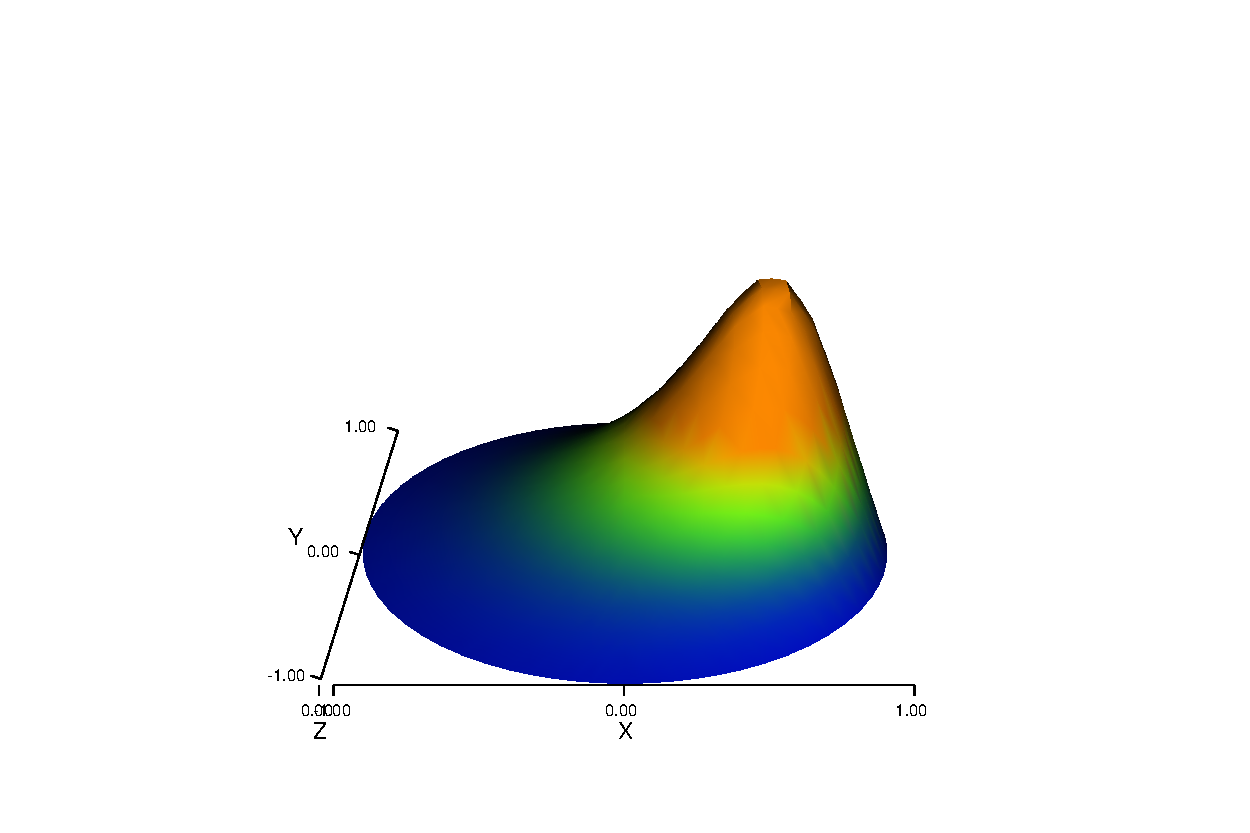
\includegraphics{chapters/langtangen/pdf/membrane_waxis.pdf}
    \caption{Plot of the deflection of a membrane.}
    \label{langtangen:poisson:2D:fig1}
  \end{center}
\end{figure}

\subsection{Combining Dirichlet and Neumann Conditions}
\label{langtangen:poisson1:DN}

Let us make a slight extension of our two-dimensional Poisson problem
from Chapter~\ref{langtangen:poisson1:bvp}
and add a Neumann boundary condition. The domain is still
the unit square, but now we set the Dirichlet condition
$u=u_0$ at the left and right sides,
$x=0$ and $x=1$, while the Neumann condition
\[ -{\partial u\over\partial n}=g \]
is applied to the remaining
sides $y=0$ and $y=1$.
The Neumann condition is also known as a \emph{natural boundary condition}
(in contrast to an essential boundary condition).

Let $\Gamma_D$ and $\Gamma_N$
denote the parts of $\partial\Omega$ where the Dirichlet and Neumann
conditions apply, respectively.
The complete boundary-value problem can be written as
\begin{eqnarray}
    - \Delta u &=& f \mbox{ in } \Omega,  \\ %\label{langtangen:poisson:2D:DN}\\
    u &=& u_0 \mbox{ on } \Gamma_D,       \\ %\label{langtangen:poisson:2D:DN}bcD\\
    - {\partial u\over\partial n} &=& g \mbox{ on } \Gamma_N  %\label{langtangen:poisson:2D:DNbcN}\langtangenep
\end{eqnarray}
Again we choose $u=1+x^2 + 2y^2$ as the exact solution and adjust $f$, $g$, and
$u_0$ accordingly:
\begin{eqnarray*}
f &=& -6,\\
g &=& \left\lbrace\begin{array}{ll}
-4, & y=1\\
0,  & y=0
\end{array}\right.\\
u_0 &=& 1 + x^2 + 2y^2\langtangenep
\end{eqnarray*}
For ease of programming we may introduce a $g$ function defined over the whole
of $\Omega$ such that $g$ takes on the right values at $y=0$ and
$y=1$. One possible extension is
\[ g(x,y) = -4y\langtangenep\]

The first task is to derive the variational problem. This time we cannot
omit the boundary term arising from the integration by parts, because
$v$ is only zero at the $\Gamma_D$. We have
\[
 -\int_\Omega v\Delta u \dx
= \int_\Omega\nabla v\cdot\nabla u\dx - \int_{\partial\Omega}v{\partial u\over
\partial n}\ds,
\]
and since $v=0$ on $\Gamma_D$,
\[
- \int_{\partial\Omega}v{\partial u\over
\partial n}\ds
=
- \int_{\Gamma_N}v{\partial u\over
\partial n}\ds
= \int_{\Gamma_N}gv\ds,
\]
by applying the boundary condition at $\Gamma_N$.
The resulting weak form reads
\begin{equation}
\int_{\Omega} \nabla v \cdot \nabla u \dx +
\int_{\Gamma_N} g v\ds
= \int_{\Omega} fv \dx\langtangenep
\label{langtangen:poisson:2D:DN:weak}
\end{equation}
Expressing \langtangenrefeq{langtangen:poisson:2D:DN:weak}
in the standard notation $a(u,v)=L(v)$ is straightforward with
\begin{eqnarray}
a(u, v) &=& \int_{\Omega} \nabla v \cdot \nabla u \dx,
\label{langtangen:poisson2:vard:a}\\
L(v) &=& \int_{\Omega} fv \dx -
\int_{\Gamma_N} g v\ds\langtangenep\label{langtangen:poisson2:vard:L}
\end{eqnarray}

How does the Neumann condition impact the implementation?
The code in the file {\fontsize{12pt}{12pt}\verb!Poisson2D_D2.py!} remains almost the same.
Only two adjustments are necessary:
\begin{enumerate}
\item The class describing the boundary where Dirichlet conditions
apply must be modified.
\item The new boundary term must be added to the expression in {\fontsize{12pt}{12pt}\verb!L!}.
\end{enumerate}
Step 1 can be coded as
\begin{Verbatim}[fontsize=\fontsize{10pt}{10pt},tabsize=8,baselinestretch=1.05,
fontfamily=tt,xleftmargin=7mm]
class DirichletBoundary(SubDomain):
    def inside(self, x, on_boundary):
        if on_boundary:
            if x[0] == 0 or x[0] == 1:
                return True
            else:
                return False
        else:
            return False
\end{Verbatim}
\noindent
A more compact implementation reads
\begin{Verbatim}[fontsize=\fontsize{10pt}{10pt},tabsize=8,baselinestretch=1.05,
fontfamily=tt,xleftmargin=7mm]
class DirichletBoundary(SubDomain):
    def inside(self, x, on_boundary):
        return on_boundary and (x[0] == 0 or x[0] == 1)
\end{Verbatim}
\noindent
We remark that testing for an exact match of real numbers,
as in {\fontsize{12pt}{12pt}\verb!x[0] == 1!}, is not good programming practice, because
small round-off errors in the computation of the {\fontsize{12pt}{12pt}\texttt{x}} values
could make the outcome {\fontsize{12pt}{12pt}\verb!False!} even though
{\fontsize{12pt}{12pt}\verb!x!} lies on the Dirichlet boundary. A better test is to
check for equality with a tolerance:
\begin{Verbatim}[fontsize=\fontsize{10pt}{10pt},tabsize=8,baselinestretch=1.05,
fontfamily=tt,xleftmargin=7mm]
class DirichletBoundary(SubDomain):
    def inside(self, x, on_boundary):
        tol = 1E-14   # tolerance for coordinate comparisons
        return on_boundary and \
               (abs(x[0]) < tol or abs(x[0] - 1) < tol)
\end{Verbatim}
\noindent

\hpl{I strongly recommend to use a function like float\_eq(a, b), which is more readable. The scitools.FloatComparison module has float\_eq (and float\_lt etc) with the possibility of adding tolerances, relative and absolute, e.g., float\_eq(x[0], 0, atol=1E-3). In geophysical applications where meter is used as unit, grid coordinates cover km and comparison with DOLFIN\_EPS is not a good idea. Then one would set float\_eq.set\_absolute\_tolerance(0.1) for instances and then all equality tests are with that tolerance.}

The second adjustment of our program concerns the definition of {\fontsize{12pt}{12pt}\texttt{L}},
where we have to add a boundary integral and a definition of the $g$
function to be integrated:
\begin{Verbatim}[fontsize=\fontsize{10pt}{10pt},tabsize=8,baselinestretch=1.05,
fontfamily=tt,xleftmargin=7mm]
g = Function(V, '-4*x[1]')
L = v*f*dx - v*g*ds
\end{Verbatim}
\noindent
The {\fontsize{12pt}{12pt}\verb!ds!} variable implies a boundary integral, while {\fontsize{12pt}{12pt}\verb!dx!}
implies an intergral over the domain $\Omega$.
No more modifications are necessary. Running the resulting program,
found in the file {\fontsize{12pt}{12pt}\verb!Poisson2D_DN1.py!}, shows a
successful verification --
$u$ equals the exact solution at all the nodes, regardless of
how many elements we use.

\subsection{Multiple Dirichlet Conditions}
\label{langtangen:poisson:multiple:Dirichlet}

The PDE problem from the previous section applies a function $u_0(x,y)$
for setting Dirichlet conditions at two parts of the boundary.
Having a single function to set multiple Dirichlet conditions is
seldom possible. The more general case is to have $m$ functions for
setting Dirichlet conditions at $m$ parts of the boundary.
The purpose of this section is to explain how such multiple conditions
are treated in FEniCS programs.

Let us
return to the case from Chapter~\ref{langtangen:poisson1:DN}
and define two separate functions for
the two Dirichlet conditions:
\begin{eqnarray*}
    - \Delta u &=& -6 \mbox{ in } \Omega, \\
    u &=& u_L \mbox{ on } \Gamma_0, \\
    u &=& u_R \mbox{ on } \Gamma_1, \\
    - {\partial u\over\partial n} &=& g \mbox{ on } \Gamma_N \langtangenep
\end{eqnarray*}
Here, $\Gamma_0$ is the boundary $x=0$, while
$\Gamma_1$ corresponds to the boundary $x=1$.
We have that $u_L = 1 + 2y^2$, $u_R = 2 + 2y^2$, and $g=-4y$.
For the left boundary $\Gamma_0$ we
define
the usual triple of a function for the boundary value,
a subclass of {\fontsize{12pt}{12pt}\texttt{SubDomain}} for defining
the boundary of interest, and a {\fontsize{12pt}{12pt}\texttt{DirichletBC}} instance:
\begin{Verbatim}[fontsize=\fontsize{10pt}{10pt},tabsize=8,baselinestretch=1.05,
fontfamily=tt,xleftmargin=7mm]
u_L = Function(V, '1 + 2*x[1]*x[1]')

class LeftDirichletBoundary(SubDomain):
    def inside(self, x, on_boundary):
        tol = 1E-14   # tolerance for coordinate comparisons
        return on_boundary and abs(x[0]) < tol

Gamma_0 = DirichletBC(V, u_L, LeftDirichletBoundary())
\end{Verbatim}
\noindent
For the boundary $x=1$ we define a similar code:
\begin{Verbatim}[fontsize=\fontsize{10pt}{10pt},tabsize=8,baselinestretch=1.05,
fontfamily=tt,xleftmargin=7mm]
u_R = Function(V, '2 + 2*x[1]*x[1]')

class RightDirichletBoundary(SubDomain):
    def inside(self, x, on_boundary):
        tol = 1E-14   # tolerance for coordinate comparisons
        return on_boundary and abs(x[0] - 1) < tol

Gamma_1 = DirichletBC(V, u_R, RightDirichletBoundary())
\end{Verbatim}
\noindent
The various essential conditions are then collected in a list
and passed onto our problem object of type {\fontsize{12pt}{12pt}\texttt{VariationalProblem}}:
\begin{Verbatim}[fontsize=\fontsize{10pt}{10pt},tabsize=8,baselinestretch=1.05,
fontfamily=tt,xleftmargin=7mm]
bc = [Gamma_0, Gamma_1]
...
problem = VariationalProblem(a, L, bc)
\end{Verbatim}
\noindent

If the $u$ values are constant at a part of the boundary, we may use
a {\fontsize{12pt}{12pt}\texttt{Constant}} instance instead of a full {\fontsize{12pt}{12pt}\texttt{Function}} instance.

The file {\fontsize{12pt}{12pt}\verb!Poisson2D_DN2.py!} contains a complete program which
demonstrates the constructions above.
An extended example with multiple Neumann conditions would have
been quite natural now, but this requires marking various parts
of the boundary using the mesh function concept and is therefore
left to Chapter~\ref{langtangen:poisson:mat:neumann}.


\subsection{A Linear Algebra Formulation}
\label{langtangen:poisson1:linalg}

Given $a(u,v)=L(v)$, the discrete solution $u$ is computed by
inserting $u=\sum_{j=1}^N U_j \phi_j$ into $a(u,v)$ and demanding
$a(u,v)=L(v)$ to be fulfilled for $N$ test functions
$\hat\phi_1,\ldots,\hat\phi_N$. This implies
\[ \sum_{j=1}^N a(\phi_j,\hat\phi_i) = L(\hat\phi_i),\quad i=1,\ldots,N,\]
which is nothing but a linear system,
\begin{displaymath}
  AU = b,
\end{displaymath}
where the entries in $A$ and $b$ are given by
\begin{displaymath}
\begin{split}
  A_{ij} &= a(\phi_j, \hat{\phi}_i), \\
  b_i &= L(\hat\phi_i)\langtangenep
\end{split}
\end{displaymath}

The examples so far have constructed a {\fontsize{12pt}{12pt}\verb!VariationalProblem!} instance
and called its {\fontsize{12pt}{12pt}\verb!solve!} method to compute the solution
{\fontsize{12pt}{12pt}\verb!u!}.
The {\fontsize{12pt}{12pt}\texttt{VariationalProblem}} instance creates a linear system
$AU=b$ and calls an appropriate solution method for such systems.
An alternative is dropping the use of a {\fontsize{12pt}{12pt}\texttt{VariationalProblem}}
instance and instead asking
\fenics{} to create the matrix $A$
and right-hand side $b$, and then solve for the
solution vector $U$ of the linear system.
The relevant statements read
\begin{Verbatim}[fontsize=\fontsize{10pt}{10pt},tabsize=8,baselinestretch=1.05,
fontfamily=tt,xleftmargin=7mm]
A = assemble(a)
b = assemble(L)
bc.apply(A, b)
u = Function(V)
solve(A, u.vector(), b)
\end{Verbatim}
\noindent
The variables {\fontsize{12pt}{12pt}\texttt{a}} and {\fontsize{12pt}{12pt}\texttt{L}} are as before, i.e., {\fontsize{12pt}{12pt}\texttt{a}} refers to the
bilinear form involving a {\fontsize{12pt}{12pt}\texttt{TrialFunction}} instance (say {\fontsize{12pt}{12pt}\texttt{u}})
and a {\fontsize{12pt}{12pt}\texttt{TestFunction}} instance ({\fontsize{12pt}{12pt}\texttt{v}}), and {\fontsize{12pt}{12pt}\texttt{L}} involves a
{\fontsize{12pt}{12pt}\texttt{TestFunction}} instance ({\fontsize{12pt}{12pt}\texttt{v}}). From {\fontsize{12pt}{12pt}\texttt{a}} and {\fontsize{12pt}{12pt}\texttt{L}}
the {\fontsize{12pt}{12pt}\texttt{assemble}} function can
compute the matrix elements $A_{i,j}$ and the vector elements $b_i$.

The matrix $A$ and vector $b$ are first assembled without incorporating
essential (Dirichlet) boundary conditions. Thereafter, the
{\fontsize{12pt}{12pt}\verb!bc.apply(A, b)!} call performs the necessary modifications to
the linear system. The first three statements above can alternatively
be carried out by\footnote{The essential boundary conditions are
now applied to the element matrices and vectors prior to assembly.}
\begin{Verbatim}[fontsize=\fontsize{10pt}{10pt},tabsize=8,baselinestretch=1.05,
fontfamily=tt,xleftmargin=7mm]
A, b = assemble_system(a, L, bc)
\end{Verbatim}
\noindent

When we have multiple Dirichlet conditions stored in a list {\fontsize{12pt}{12pt}\texttt{bc}},
as explained in
Chapter~\ref{langtangen:poisson:multiple:Dirichlet}, we must apply
each condition in {\fontsize{12pt}{12pt}\texttt{bc}} to the system:
\begin{Verbatim}[fontsize=\fontsize{10pt}{10pt},tabsize=8,baselinestretch=1.05,
fontfamily=tt,xleftmargin=7mm]
# bc is a list of DirichletBC instances
for condition in bc:
    condition.apply(A, b)
\end{Verbatim}
\noindent
Alternatively, we can make the call
\begin{Verbatim}[fontsize=\fontsize{10pt}{10pt},tabsize=8,baselinestretch=1.05,
fontfamily=tt,xleftmargin=7mm]
A, b = assemble_system(a, L, bc)
\end{Verbatim}
\noindent

Note that the solution {\fontsize{12pt}{12pt}\verb!u!} is, as before, a {\fontsize{12pt}{12pt}\verb!Function!} instance.
The degrees of freedom, $U=A^{-1}b$, are filled
into {\fontsize{12pt}{12pt}\texttt{u}}'s {\fontsize{12pt}{12pt}\texttt{Vector}} instance ({\fontsize{12pt}{12pt}\texttt{u.vector()}})
by the {\fontsize{12pt}{12pt}\verb!solve!} function.

The object {\fontsize{12pt}{12pt}\verb!A!} is of type {\fontsize{12pt}{12pt}\verb!Matrix!}, while {\fontsize{12pt}{12pt}\verb!b!} and
{\fontsize{12pt}{12pt}\verb!u.vector()!} are of type {\fontsize{12pt}{12pt}\verb!Vector!}. We may convert the
matrix and vector data to {\fontsize{12pt}{12pt}\verb!numpy!} arrays by calling the
{\fontsize{12pt}{12pt}\verb!array()!} method as shown before. If you wonder how essential
boundary conditions are incorporated in the linear system, you can
print out {\fontsize{12pt}{12pt}\texttt{A}} and {\fontsize{12pt}{12pt}\texttt{b}} before and after the
{\fontsize{12pt}{12pt}\texttt{bc.apply(A, b)}} call:
\begin{Verbatim}[fontsize=\fontsize{10pt}{10pt},tabsize=8,baselinestretch=1.05,
fontfamily=tt,xleftmargin=7mm]
if mesh.numCells() < 16:  # print for small meshes only
    print A.array()
    print b.array()
bc.apply(A, b)
if mesh.numCells() < 16:
    print A.array()
    print b.array()
\end{Verbatim}
\noindent
You will see that {\fontsize{12pt}{12pt}\texttt{A}} is modified in a symmetric way:
for each degree of freedom that is known, the corresponding row
and column is zero'ed out and 1 is placed on the main diagonal.
The right-hand side {\fontsize{12pt}{12pt}\texttt{b}} is modified accordingly (the column times
the value of the degree of freedom is subtracted from {\fontsize{12pt}{12pt}\texttt{b}}, and
then the corresponding entry in {\fontsize{12pt}{12pt}\texttt{b}} is replaced by the known value
of the degree of freedom).

Sometimes it can be handy to transfer the linear system to Matlab or Octave
for futher analysis, e.g., computation of eigenvalues of $A$.
This is easily done by opening
a {\fontsize{12pt}{12pt}\texttt{File}} instance with a filename extension {\fontsize{12pt}{12pt}\texttt{.m}} and dump
the {\fontsize{12pt}{12pt}\texttt{Matrix}} and {\fontsize{12pt}{12pt}\texttt{Vector}} instances as follows:
\begin{Verbatim}[fontsize=\fontsize{10pt}{10pt},tabsize=8,baselinestretch=1.05,
fontfamily=tt,xleftmargin=7mm]
mfile = File('A.m'); mfile << A
mfile = File('b.m'); mfile << b
\end{Verbatim}
\noindent
The data files {\fontsize{12pt}{12pt}\texttt{A.m}} and {\fontsize{12pt}{12pt}\texttt{b.m}} can be loaded directly into
Matlab or Octave.

The complete code where our Poisson problem is solved by forming
the linear system $AU=b$ explicitly, is stored in the files
{\fontsize{12pt}{12pt}\verb!Poisson2D_DN_la1.py!} (one common Dirichlet condition) and
{\fontsize{12pt}{12pt}\verb!Poisson2D_DN_la2.py!} (two separate Dirichlet conditions).

Creating the linear system
explicitly in the user's program, as an alternative to
using a {\fontsize{12pt}{12pt}\texttt{VariationalProblem}} instance, can have some advantages in more
advanced problem settings. For example, $A$ may be constant throughout
a time-dependent simulation, so we can avoid recalculating $A$ at
every time level and save a significant amount of simulation time.
Chapters \ref{langtangen:timedep:diffusion1:impl} and
\ref{langtangen:timedep:diffusion1:noassemble} deal with this topic in detail.

%In other problems, we may divide the variational
%problem and linear system into different terms, say $A=M + \Delta t K$,
%where $M$ is a matrix arising from a term like $\partial u/\partial t$,
%$K$ is a term corresponding to a Laplace operator, and $\Delta t$ is
%a time discretization parameter. When $\Delta t$ is changed in time,
%we can efficiently recompute $A = M + \Delta t K$ without
%reassembling the constant matrices $M$ and $K$. This strategy may
%speed up simulations significantly.


\subsection{A Variable-Coefficient Poisson Problem}
\label{langtangen:possion:2D:varcoeff}

Suppose we have a variable coefficient $p(x,y)$ in the Laplace operator,
as in the boundary-value problem
\begin{equation} \label{langtangen:poisson:2D:varcoeff}
  \begin{array}{rcll}
    - \nabla\cdot \left\lbrack
p(x,y)\nabla u(x,y)\right\rbrack &=& f(x,y) &\mbox{in } \Omega, \\
    u(x,y) &=& u_0(x,y) &\mbox{on } \partial\Omega\langtangenep
  \end{array}
\end{equation}
We shall quickly demonstrate that this simple extension of our model
problem only requires an equally simple extension of the \fenics{} program.

Let us continue to use our favorite solution $u(x,y)=1+x+2y^2$ and
then prescribe $p(x,y)=x+y$. It follows that
$u_0(x,y) = 1 + x^2 + 2y^2$ and $f(x,y)=-8x-10y$.

What are the modifications we need to do in the {\fontsize{12pt}{12pt}\verb!Poisson2D_D2.py!} program
from Chapter~\ref{langtangen:poisson1:verify1}?
\begin{enumerate}
\item {\fontsize{12pt}{12pt}\texttt{f}} must be a {\fontsize{12pt}{12pt}\texttt{Function}} since it is no longer a constant,
\item a new {\fontsize{12pt}{12pt}\texttt{Function}} {\fontsize{12pt}{12pt}\texttt{p}} must be defined for the variable coefficient,
\item the variational problem is slightly changed.
\end{enumerate}
First we address the modified variational problem. Multiplying
the PDE in \langtangenrefeq{langtangen:poisson:2D:varcoeff} and
integrating by parts now results
in
\[ \int_\Omega p\nabla v\cdot\nabla u\dx -
\int_{\partial\Omega} pv{\partial u\over
\partial n}\ds = \int_\Omega vf\dx\langtangenep\]
The function spaces for $u$ and $v$ are the same as in
Chapter~\ref{langtangen:poisson1:varform}, implying that the boundary integral
vanishes since $v=0$ on $\partial\Omega$ where we have Dirichlet conditions.
The weak form $a(u,v)=L(v)$ then has
\begin{eqnarray}
a(u,v) &=& \int_\Omega p\nabla v\cdot\nabla u\dx,\\
L(v) &=& \int_\Omega vf\dx\langtangenep
\end{eqnarray}
In the code from Chapter~\ref{langtangen:poisson1:impl} we must replace
\begin{Verbatim}[fontsize=\fontsize{10pt}{10pt},tabsize=8,baselinestretch=1.05,
fontfamily=tt,xleftmargin=7mm]
a = dot(grad(v), grad(u))*dx
\end{Verbatim}
\noindent
by
\begin{Verbatim}[fontsize=\fontsize{10pt}{10pt},tabsize=8,baselinestretch=1.05,
fontfamily=tt,xleftmargin=7mm]
a = p*dot(grad(v), grad(u))*dx
\end{Verbatim}
\noindent
The definitions of {\fontsize{12pt}{12pt}\texttt{p}} and {\fontsize{12pt}{12pt}\texttt{f}} read
\begin{Verbatim}[fontsize=\fontsize{10pt}{10pt},tabsize=8,baselinestretch=1.05,
fontfamily=tt,xleftmargin=7mm]
p = Function(V, 'x[0] + x[1]')
f = Function(V, '-8*x[0] - 10*x[1]')
\end{Verbatim}
\noindent
No additional modifications are necessary. The complete code can be
found in in the file {\fontsize{12pt}{12pt}\verb!Poisson2D_Dvc.py!}. You can run it and confirm
that it recovers the exact $u$ at the nodes.

The flux $-p\nabla u$ may be of particular interest in variable-coefficient
Poisson
problems. As explained in Chapter~\ref{langtangen:poisson:gradu},
we normally want the piecewise discontinuous flux or gradient
to be approximated by a continuous vector field, using the same elements
as used for the numerical solution $u$. The approximation now consists of
solving $w = -p\nabla u$ by a finite element method:
find $w\in V^{(g)}_h$ such that
\begin{equation}
a(w, v) = L(v^{g})\quad\forall v\in \hat{V}_h^{(g)},
\end{equation}
where
\begin{eqnarray}
a(w, v) &=& \int_\Omega w\cdot v\dx,\\
L(v^{g}) &=& \int_\Omega v\cdot (-p \nabla u)\dx\langtangenep
\end{eqnarray}
This problem is identical to the one in Chapter~\ref{langtangen:poisson:gradu},
except that $p$ enters the integral in $L$.

The relevant Python statements for computing the flux field take the form
\begin{Verbatim}[fontsize=\fontsize{10pt}{10pt},tabsize=8,baselinestretch=1.05,
fontfamily=tt,xleftmargin=7mm]
V_g = VectorFunctionSpace(mesh, 'CG', 1)
v = TestFunction(V_g)
w = TrialFunction(V_g)

a = dot(w, v)*dx
L = dot(-p*grad(u), v)*dx
problem = VariationalProblem(a, L)
flux = problem.solve()
\end{Verbatim}
\noindent
The convenience function {\fontsize{12pt}{12pt}\texttt{project}} was made to condense the frequently
occuring statements above:
\begin{Verbatim}[fontsize=\fontsize{10pt}{10pt},tabsize=8,baselinestretch=1.05,
fontfamily=tt,xleftmargin=7mm]
flux = project(-p*grad(u),
               VectorFunctionSpace(mesh, 'CG', 1))
\end{Verbatim}
\noindent

Plotting the flux vector field is naturally as easy as plotting
the gradient in Chapter~\ref{langtangen:poisson:gradu}:
\begin{Verbatim}[fontsize=\fontsize{10pt}{10pt},tabsize=8,baselinestretch=1.05,
fontfamily=tt,xleftmargin=7mm]
plot(flux, title='flux field')

flux_x, flux_y = flux.split(deepcopy=True)  # extract components
plot(flux_x, title='x-component of flux (-p*grad(u))')
plot(flux_y, title='y-component of flux (-p*grad(u))')
\end{Verbatim}
\noindent

Data analysis of the nodal values of the flux field may conveniently
apply the underlying {\fontsize{12pt}{12pt}\texttt{numpy}} arrays:
\begin{Verbatim}[fontsize=\fontsize{10pt}{10pt},tabsize=8,baselinestretch=1.05,
fontfamily=tt,xleftmargin=7mm]
flux_x_array = flux_x.vector().array()
flux_y_array = flux_y.vector().array()
\end{Verbatim}
\noindent

The program {\fontsize{12pt}{12pt}\verb!Poisson2D_Dvc.py!} contains in addition some plots,
including a curve plot
comparing {\fontsize{12pt}{12pt}\verb!flux_x!} and the exact counterpart along the line $y=1/2$.
The associated programming details related to this visualization
are explained in Chapter~\ref{langtangen:structviz}.

\subsection{Visualization of Structured Mesh Data}
\label{langtangen:structviz}

When finite element computations are done on
a structured rectangular mesh, maybe with uniform partitioning,
VTK-based tools for completely unstructured 2D/3D meshes are not required.
Instead we can use visualization
tools for structured data, like the data appearing
in finite difference simulations and image analysis.
We shall demonstrate the potential of such tools.

A necessary first step
is to transform our {\fontsize{12pt}{12pt}\texttt{mesh}} instance to an object representing a
rectangle with equally-shaped \emph{rectangular} cells.
The Python package {\fontsize{12pt}{12pt}\texttt{scitools}} has this type of structure, called
a {\fontsize{12pt}{12pt}\texttt{UniformBoxGrid}}. The second step is to transform the
one-dimensional array of nodal
values to a two-dimensional array holding the values at
the corners of the cells in the structured grid. In such
grids, we want to access a value by its $i$ and $j$ indices, $i$ counting
cells in the $x$ direction, and $j$ counting cells in the $y$ direction.
This transformation is in principle straiightforward, yet it frequently leads to
obscure indexing errors. The {\fontsize{12pt}{12pt}\texttt{BoxField}} object in {\fontsize{12pt}{12pt}\texttt{scitools}}
takes conveniently care of the details of the transformation.
With a {\fontsize{12pt}{12pt}\texttt{BoxField}} defined on a {\fontsize{12pt}{12pt}\texttt{UniformBoxGrid}} it is very easy to
call up more standard plotting packages to visualize the solution along
lines in the domain or as 2D contours or lifted surfaces.

Let us go back to the {\fontsize{12pt}{12pt}\verb!Poisson2D_Dvc.py!} code from
Chapter~\ref{langtangen:possion:2D:varcoeff} and map {\fontsize{12pt}{12pt}\texttt{u}} onto a
{\fontsize{12pt}{12pt}\texttt{BoxField}} instance:
\begin{Verbatim}[fontsize=\fontsize{10pt}{10pt},tabsize=8,baselinestretch=1.05,
fontfamily=tt,xleftmargin=7mm]
from scitools.BoxField import *
u_box = dolfin_function2BoxField(u, mesh, (nx,ny), uniform_mesh=True)
\end{Verbatim}
\noindent
Here, {\fontsize{12pt}{12pt}\texttt{nx}} and {\fontsize{12pt}{12pt}\texttt{ny}} are the number of divisions in each space
direction that were used when calling {\fontsize{12pt}{12pt}\texttt{UnitSquare}} to make the
{\fontsize{12pt}{12pt}\texttt{mesh}} instance.
The result {\fontsize{12pt}{12pt}\verb!u_box!} is a {\fontsize{12pt}{12pt}\texttt{BoxField}}
instance that supports ``finite difference'' indexing and an underlying
grid suitable for {\fontsize{12pt}{12pt}\texttt{numpy}} operations on 2D data.
Also 1D and 3D functions in \dolfin{} can be turned
into {\fontsize{12pt}{12pt}\texttt{BoxField}} instances.

The ability to access a finite element field in the way one can access
a finite difference-type of field is handy in many occasions, including
visualization and data analysis.
Here is an example of writing out the coordinates and the field value
at a grid point with indices {\fontsize{12pt}{12pt}\texttt{i}} and {\fontsize{12pt}{12pt}\texttt{j}} (going from 0 to
{\fontsize{12pt}{12pt}\texttt{nx}} and {\fontsize{12pt}{12pt}\texttt{ny}}, respectively, from lower left to upper right corner):
\begin{Verbatim}[fontsize=\fontsize{10pt}{10pt},tabsize=8,baselinestretch=1.05,
fontfamily=tt,xleftmargin=7mm]
i = nx; j = ny   # upper right corner
print 'u(%g,%g)=%g' % (u_box.grid.coor[X][i],
                       u_box.grid.coor[Y][j],
                       u_box.values[i,j])
\end{Verbatim}
\noindent
For instance,
the $x$ coordinates are reached by {\fontsize{12pt}{12pt}\verb!u_box.grid.coor[X]!}, where
{\fontsize{12pt}{12pt}\texttt{X}} is an integer (0) imported from {\fontsize{12pt}{12pt}\texttt{scitools.BoxField}}.
The {\fontsize{12pt}{12pt}\texttt{grid}} attribute is an instance of class {\fontsize{12pt}{12pt}\texttt{UniformBoxGrid}}.

Many plotting programs can be used to visualize the data in
{\fontsize{12pt}{12pt}\verb!u_box!}.  Matplotlib is now a very popular plotting program in
the Python world and could be used to make contour plots of
{\fontsize{12pt}{12pt}\verb!u_box!}. However, other programs like Gnuplot, VTK, and Matlab have better
support for surface plots. Our choice in this tutorial is to use the
Python package {\fontsize{12pt}{12pt}\texttt{scitools.easyviz}}, which offers a uniform
Matlab-like syntax to various plotting packages such as Gnuplot,
Matplotlib, VTK, OpenDX, Matlab, and others. With {\fontsize{12pt}{12pt}\texttt{scitools.easyviz}} we
write one set of statements, close to what one would do in Matlab or
Octave, and then it is easy to switch between different plotting
programs, at a later stage, through a command-line option, a line in a
configuration file, or an import statement in the program.  By
default, {\fontsize{12pt}{12pt}\texttt{scitools.easyviz}} employs Gnuplot as plotting program,
and this is a highly relevant choice for scalar fields over two-dimensional,
structured meshes, or for curve plots along lines through the domain.

A contour plot is made by the following {\fontsize{12pt}{12pt}\texttt{scitools.easyviz}} command:
\begin{Verbatim}[fontsize=\fontsize{10pt}{10pt},tabsize=8,baselinestretch=1.05,
fontfamily=tt,xleftmargin=7mm]
from scitools.easyviz import contour, title, hardcopy
contour(u_box.grid.coorv[X], u_box.grid.coorv[Y], u_box.values,
        5, clabels='on')
title('Contour plot of u')
hardcopy('u_contours.pdf')

# or more compact syntax:
contour(u_box.grid.coorv[X], u_box.grid.coorv[Y], u_box.values,
        5, clabels='on',
        hardcopy='u_contours.pdf', title='Contour plot of u')
\end{Verbatim}
\noindent
The resulting plot can be viewed in Figure~\ref{langtangen:poisson:2D:fig2}a.
The {\fontsize{12pt}{12pt}\texttt{contour}} function needs arrays with the $x$ and $y$ coordinates
expanded to 2D arrays (in the same way as demanded when
making vectorized
{\fontsize{12pt}{12pt}\texttt{numpy}} calculations of arithmetic expressions over all grid points).
The correctly expanded arrays are stored in {\fontsize{12pt}{12pt}\texttt{grid.coorv}}.
The above call to
{\fontsize{12pt}{12pt}\texttt{contour}} creates 5 equally spaced contour lines, and with
{\fontsize{12pt}{12pt}\texttt{clabels='on'}} the contour values can be seen in the plot.

Other functions for visualizing 2D scalar fields are {\fontsize{12pt}{12pt}\texttt{surf}} and
{\fontsize{12pt}{12pt}\texttt{mesh}} as known from Matlab. Because the {\fontsize{12pt}{12pt}\texttt{from dolfin import *}}
statement imports several names that are also present
in {\fontsize{12pt}{12pt}\texttt{scitools.easyviz}} (e.g., {\fontsize{12pt}{12pt}\texttt{plot}}, {\fontsize{12pt}{12pt}\texttt{mesh}}, and
{\fontsize{12pt}{12pt}\texttt{figure}}), we use functions from the latter package through a
module prefix {\fontsize{12pt}{12pt}\texttt{ev}} (for \underline{e}asy\underline{v}iz) from now on:
\begin{Verbatim}[fontsize=\fontsize{10pt}{10pt},tabsize=8,baselinestretch=1.05,
fontfamily=tt,xleftmargin=7mm]
import scitools.easyviz as ev
ev.figure()
ev.surf(u_box.grid.coorv[X], u_box.grid.coorv[Y], u_box.values,
        shading='interp', colorbar='on',
        title='surf plot of u', hardcopy='u_surf.pdf')

ev.figure()
ev.mesh(u_box.grid.coorv[X], u_box.grid.coorv[Y], u_box.values,
        title='mesh plot of u', hardcopy='u_mesh.pdf')
\end{Verbatim}
\noindent
Figure~\ref{langtangen:poisson:2D:fig3} exemplifies the surfaces arising from
the two plotting commands above.
You can type
{\fontsize{12pt}{12pt}\texttt{pydoc scitools.easyviz}} in a terminal window
to get a full tutorial.

A handy feature of {\fontsize{12pt}{12pt}\texttt{BoxField}} is the ability to give a start point
in the grid and a direction, and then extract the field and corresponding
coordinates along the nearst grid
line. In 3D fields
one can also extract data in a plane.
Say we
want to plot $u$ along the line $y=1/2$ in the grid. The grid points,
{\fontsize{12pt}{12pt}\texttt{x}}, and the
$u$ values along this line, {\fontsize{12pt}{12pt}\texttt{uval}}, are extracted by
\begin{Verbatim}[fontsize=\fontsize{10pt}{10pt},tabsize=8,baselinestretch=1.05,
fontfamily=tt,xleftmargin=7mm]
start = (0, 0.5)
x, uval, y_fixed, snapped = u_box.gridline(start, direction=X)
\end{Verbatim}
\noindent
The variable {\fontsize{12pt}{12pt}\texttt{snapped}} is true if the line had to be snapped onto a
gridline and in that case {\fontsize{12pt}{12pt}\verb!y_fixed!} holds the snapped
(altered) $y$ value.
Plotting $u$ versus the $x$ coordinate along this line, using
{\fontsize{12pt}{12pt}\texttt{scitools.easyviz}}, is now a matter of
\begin{Verbatim}[fontsize=\fontsize{10pt}{10pt},tabsize=8,baselinestretch=1.05,
fontfamily=tt,xleftmargin=7mm]
ev.figure()  # new plot window
ev.plot(x, uval, 'r-')  # 'r--: red solid line
ev.title('Solution')
ev.legend('finite element solution')

# or more compactly:
ev.plot(x, uval, 'r-', title='Solution',
        legend='finite element solution')
\end{Verbatim}
\noindent

A more exciting plot compares the projected numerical flux in
$x$ direction along the
line $y=1/2$ with the exact flux:
\begin{Verbatim}[fontsize=\fontsize{10pt}{10pt},tabsize=8,baselinestretch=1.05,
fontfamily=tt,xleftmargin=7mm]
ev.figure()
flux_x_box = dolfin_function2BoxField(flux_x, mesh, (nx,ny),
                                      uniform_mesh=True)
x, fluxval, y_fixed, snapped = \
      flux_x_box.gridline(start, direction=X)
y = y_fixed
flux_x_exact = -(x + y)*2*x
ev.plot(x, fluxval, 'r-',
        x, flux_x_exact, 'b-',
        legend=('numerical (projected) flux', 'exact flux'),
        title='Flux in x-direction (at y=%g)' % y_fixed,
        hardcopy='flux.pdf')
\end{Verbatim}
\noindent
As seen from Figure~\ref{langtangen:poisson:2D:fig2}b, the numerical flux
is accurate except in the elements closest to the boundaries.

\begin{figure}
  \begin{center}
    \centerline{
      \subfloat[]{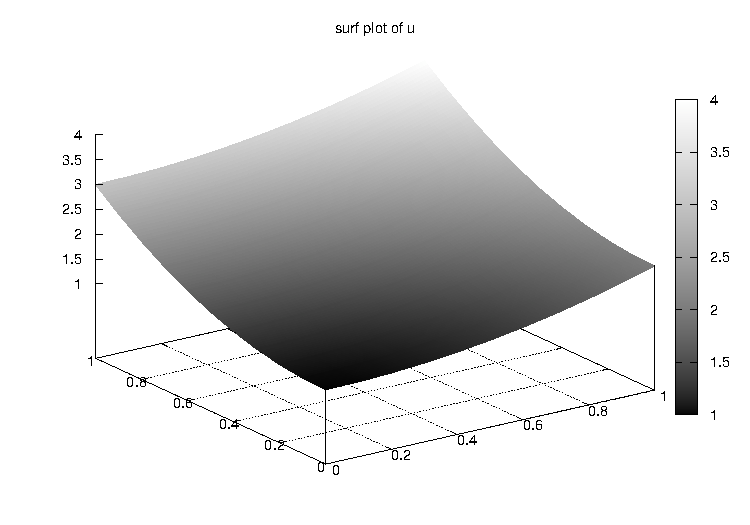
\includegraphics[width=0.9\linewidth]{chapters/langtangen/pdf/Poisson2D_Dvc_surf1.pdf}}}
    \centerline{
      \subfloat[]{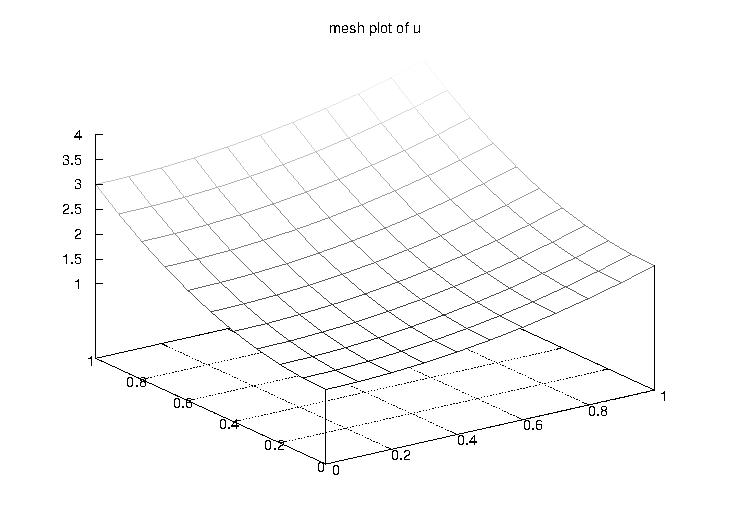
\includegraphics[width=0.9\linewidth]{chapters/langtangen/pdf/Poisson2D_Dvc_mesh1.pdf}}}
    \caption{Examples on plots created by transforming the finite element field to
      a field on a uniform, structured 2D grid:
      (a) a surface plot of the solution; (b) lifted mesh plot of the solution.
    }
    \label{langtangen:poisson:2D:fig3}
  \end{center}
\end{figure}

\begin{figure}
  \begin{center}
    \centerline{
      \subfloat[]{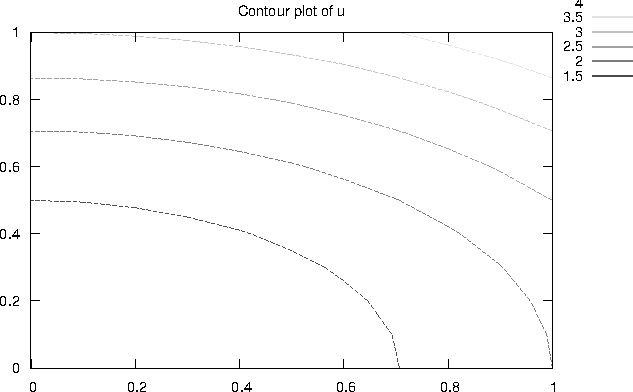
\includegraphics[width=0.9\linewidth]{chapters/langtangen/pdf/Poisson2D_Dvc_contour1.pdf}}}
    \centerline{
      \subfloat[]{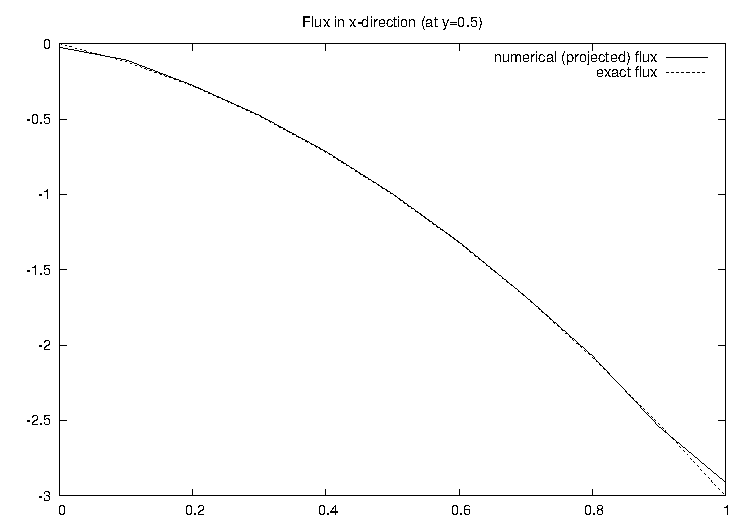
\includegraphics[width=0.8\linewidth]{chapters/langtangen/pdf/Poisson2D_Dvc_flux_x.pdf}}
    }
    \caption{  Examples on plots created by transforming the finite element field to
      a field on a uniform, structured 2D grid:
      (a) contour plot of the solution; (b) curve plot of the exact flux
      $-p\partial u/\partial x$ against the corresponding projected numerical flux.
    }
    \label{langtangen:poisson:2D:fig2}
  \end{center}
\end{figure}

It should be easy with the information above to a transform finite element
field over a uniform rectangular or box-shaped mesh to the corresponding
{\fontsize{12pt}{12pt}\texttt{BoxField}} instance and perform Matlab-style
visualizations of the whole field or
the field over planes or along lines through the domain.
By the transformation to a regular grid we have some more flexibility
than what Viper offers. (It should be added that
comprehensive tools like
VisIt, MayaVi2, or ParaView also have the possibility for plotting fields
along lines and extracting planes in 3D geometries, though usually with
less degree of control compared to Gnuplot, Matlab, and Matplotlib.)

\subsection{Parameterizing the Number of Space Dimensions}
\label{langtangen:poisson:nD}

\fenics{} makes it is easy to write a unified simulation code that can operate
in 1D, 2D, and 3D. We will conveniently make use of this feature in
forthcoming examples. The relevant technicalities are therefore explained
below.

Consider the simple problem
\begin{equation}
u''(x) = 2\hbox{ in }[0,1],\quad u(0)=0,\ u(1)=0,
\end{equation}
with exact solution $u(x)=x^2$. Our aim is to formulate and solve this
problem in a 2D and a 3D domain as well.
We may generalize the domain $[0,1]$ to a box of any size
in the $y$ and $z$ directions and pose homogeneous Neumann
conditions $\partial u/\partial n = 0$ at all additional boundaries
$y=\mbox{const}$ and $z=\mbox{const}$ to ensure that $u$ only varies with
$x$. For example, let us choose
a unit hypercube as domain: $\Omega = [0,1]^d$, where $d$ is the number
of space dimensions. The generalized $d$-dimensional Poisson problem
then reads
\begin{equation} \label{langtangen:poisson1:ddim}
  \begin{array}{rcll}
    \Delta u &=& 2 &\mbox{in } \Omega, \\
    u &=& 0 &\mbox{on } \Gamma_0,\\
    u &=& 1 &\mbox{on } \Gamma_1,\\
{\partial u\over\partial n} &=& 0 &\mbox{on } \partial\Omega\cap\left(
\Gamma_0\cup\Gamma_1\right),
  \end{array}
\end{equation}
where $\Gamma_0$ is the side of the hypercube where $x=0$, and
where $\Gamma_1$ is the side where $x=1$.

Implementing \langtangenrefeq{langtangen:poisson1:ddim} for any $d$ is no more
complicated than solving a dimension-specific problem.
The only non-trivial part of the code is actually to define the mesh.
We use the command line to provide user-input to the program. The first argument
can be the degree of the polynomial in the finite element basis functions.
Thereafter, we supply the
cell divisions in the various spatial directions. The number of
command-line arguments will then imply the number of space dimensions.
For example, writing {\fontsize{12pt}{12pt}\texttt{3 10 3 4}} on the command-line means that
we want to approximate $u$ by piecewise polynomials of degree 3,
and that the domain is a three-dimensional cube with $10\times 3\times 4$
divisions in the $x$, $y$, and $z$ directions, respectively.
Each of the $10\times 3\times 4 = 120$ boxes will
be divided into six tetrahedras.
The Python code can be quite compact:
\begin{Verbatim}[fontsize=\fontsize{10pt}{10pt},tabsize=8,baselinestretch=1.05,
fontfamily=tt,xleftmargin=7mm]
degree = int(sys.argv[1])
divisions = [int(arg) for arg in sys.argv[2:]]
d = len(divisions)
domain_type = [UnitInterval, UnitSquare, UnitCube]
mesh = domain_type[d-1](*divisions)
V = FunctionSpace(mesh, 'CG', degree)
\end{Verbatim}
\noindent
First note that although {\fontsize{12pt}{12pt}\texttt{sys.argv[2:]}} holds the divisions of
the mesh, all elements of the list {\fontsize{12pt}{12pt}\texttt{sys.argv[2:]}} are string objects,
so we need to explicitly convert each element to an integer.
The construction {\fontsize{12pt}{12pt}\verb!domain_type[d-1]!} will pick the right name of the
object used to define the domain and generate the mesh.
Moreover, the argument {\fontsize{12pt}{12pt}\texttt{*divisions}}
sends each component of the list {\fontsize{12pt}{12pt}\texttt{divisions}} as a separate
argument. For example, in a 2D problem where {\fontsize{12pt}{12pt}\texttt{divisions}} has
two elements, the statement
\begin{Verbatim}[fontsize=\fontsize{10pt}{10pt},tabsize=8,baselinestretch=1.05,
fontfamily=tt,xleftmargin=7mm]
mesh = domain_type[d-1](*divisions)
\end{Verbatim}
\noindent
is equivalent to
\begin{Verbatim}[fontsize=\fontsize{10pt}{10pt},tabsize=8,baselinestretch=1.05,
fontfamily=tt,xleftmargin=7mm]
mesh = UnitSquare(divisions[0], divisions[1])
\end{Verbatim}
\noindent

The next part of the program is to set up the boundary conditions.
Since the Neumann conditions have $\partial u/\partial n=0$ we can
omit the boundary integral from the weak form. We then only
need to take care of Dirichlet conditions at two sides:
\begin{Verbatim}[fontsize=\fontsize{10pt}{10pt},tabsize=8,baselinestretch=1.05,
fontfamily=tt,xleftmargin=7mm]
tol = 1E-14   # tolerance for coordinate comparisons
class DirichletBoundary0(SubDomain):
    def inside(self, x, on_boundary):
        return on_boundary and abs(x[0]) < tol

class DirichletBoundary1(SubDomain):
    def inside(self, x, on_boundary):
        return on_boundary and abs(x[0] - 1) < tol

bc0 = DirichletBC(V, Constant(mesh, 0), DirichletBoundary0())
bc1 = DirichletBC(V, Constant(mesh, 1), DirichletBoundary1())
bc = [bc0, bc1]
\end{Verbatim}
\noindent
Note that this code is independent of the number of space dimensions.
So are the statements defining and solving
the variational problem:
\begin{Verbatim}[fontsize=\fontsize{10pt}{10pt},tabsize=8,baselinestretch=1.05,
fontfamily=tt,xleftmargin=7mm]
v = TestFunction(V)
u = TrialFunction(V)
f = Constant(mesh, -2)
a = dot(grad(v), grad(u))*dx
L = v*f*dx

problem = VariationalProblem(a, L, bc)
u = problem.solve()
\end{Verbatim}
\noindent
The complete code is found in {\fontsize{12pt}{12pt}\verb!Poisson123D_DN1.py!}.

Observe that if we actually want to test variations in one selected
space direction, parameterized by {\fontsize{12pt}{12pt}\texttt{e}}, we only need to
replace {\fontsize{12pt}{12pt}\texttt{x[0]}} in the code by {\fontsize{12pt}{12pt}\texttt{x[e]}} (!). The parameter
{\fontsize{12pt}{12pt}\texttt{e}} could be given as the second command-line argument.
This extension appears in the file {\fontsize{12pt}{12pt}\verb!Poisson123D_DN2.py!}.
You can run a 3D problem with this code where $u$ varies in, e.g.,
$z$ direction and is approximated by, e.g., a 5-th degree polynomial.
For any legal input the numerical solution coincides with the
exact solution at the nodes (because the exact solution is a second-order
polynomial).


%\subsection{DIV}
%
%Function with eval method (see dielectric example), e.g.,
%f=1 in a small region and 0 elsewhere.
%Or: MeshFunction with markers.
%
%Operations on Functions: - + *, not just numpy arrays, but the Function
%itself - test! (dielectric has u - exact, and they are in different
%spaces :-)

\section{Nonlinear Problems}
\label{langtangen:poisson:nonlinear}

%See Chapter~\ref{sec:abstract,nonlinear}!


Now we shall address how to solve nonlinear PDEs in \fenics. Our
sample PDE for implementation is taken as a nonlinear Poisson equation:
\begin{equation}
-\nabla\cdot\left( q(u)\nabla u\right) = f\langtangenep
\end{equation}
The coefficient $q(u)$ makes the equation nonlinear (unless $q(u)$
is a constant).

To be able to easily verify our implementation,
we choose the domain, $q(u)$, $f$, and the boundary
conditions such that we have
a simple, exact solution $u$. Let
$\Omega$ is the unit hypercube $[0, 1]^d$
in $d$ dimensions, $q(u)=(1+u)^m$, $f=0$, $u=0$ for $x_0=0$, $u=1$
for $x_0=1$, and $\partial u/\partial n=0$ at all other boundaries
$x_i=0$ and $x_i=1$, $i=1,\ldots,d-1$. The coordinates are now represented by
the symbols $x_0,\ldots,x_{d-1}$. The exact solution is then
\begin{equation}
u(x_0,\ldots,x_d) = \left((2^{m+1}-1)x_0 + 1\right)^{1/(m+1)} - 1\langtangenep
\end{equation}

The variational formulation of our model problem reads:
Find $u \in V$ such that
\begin{equation} \label{langtangen:poisson:nonlinear}
  F(u; v) = 0 \quad \forall v \in \hat{V},
\end{equation}
where
\begin{equation}
\label{langtangen:poisson:nonlinear2}
F(u; v) = \int_\Omega \nabla v\cdot\left( q(u)\nabla u\right)\dx,
\end{equation}
and
\begin{displaymath}
  \begin{split}
    \hat{V} &= \{v \in H^1(\Omega) : v = 0 \mbox{ on } x_0=0\mbox{ and }x_0=1\}, \\
     V      &= \{v \in H^1(\Omega) : v = 0 \mbox{ on } x_0=0\mbox{ and } v = 1\mbox{ on }x_0=1\}. \\
  \end{split}
\end{displaymath}
The discrete problem arises as usual by restricting $V$ and $\hat V$ to a
pair of discrete spaces: Find $u_h\in V_h$ such that
\begin{equation}
  F(u_h; v) = 0 \quad \forall v \in \hat{V}_h,
\label{langtangen:poisson:nonlinear:d}
\end{equation}
with $u_h = \sum_{j=1}^N U_j \phi_j$. Since $F$ is a nonlinear function
of $u_h$, \langtangenrefeq{langtangen:poisson:nonlinear:d} gives rise to a system of
nonlinear algebraic equations.
From now on the interest is only in the discrete problem, and as mentioned
in Chapter~\ref{langtangen:poisson1:varform},
we simply write $u$ instead of $u_h$ to get a closer notation between
the mathematics and the Python code. When the exact solution needs to
be distinguished, we denote it by $u_e$.

\fenics{} can be used in alternative ways for solving a nonlinear PDE
problem. We shall in the following subsections go through four
solution strategies:
1) a simple Picard-type iteration,
2) a Newton method at the algebraic level,
3) a Newton method at the PDE level, and
4) an automatic approach where \fenics{} attacks the nonlinear variational
problem directly. The ``black box'' strategy 4) is definitely the
simplest one from a
programmer's point of view, but the others give more control of the
solution process for nonlinear equations (which also has some
pedagogical advantages).

\subsection{Picard Iteration}
\label{langtangen:nonlinear:Picard}

Picard iteration is an easy way of handling nonlinear PDEs: we simply
use a known, previous solutions in the nonlinear terms such that these
terms become linear in the unknown $u$.
For our particular problem,
this means that we use a known, previous solution in the coefficient $q(u)$.
More precisely, given a solution $u^k$ from iteration $k$, we seek a
new (hopefully improved) solution $u^{k+1}$ in iteration $k+1$ such
that $u^{k+1}$ solves the \emph{linear problem}
\begin{equation}
\label{langtangen:poisson:nonlinear:picard1}
\nabla\cdot \left(q(u^k)\nabla u^{k+1}\right) = 0,\quad k=0,1,\ldots
\end{equation}
The iterations require an initial guess $u^0$.
The hope is that $u^{k} \rightarrow u$ as $k\rightarrow\infty$, and that
$u^{k+1}$ is sufficiently close to the exact
solution $u$ of the discrete problem after just a few iterations.

We can easily formulate a variational problem for $u^{k+1}$ from
Equation~\langtangenrefeq{langtangen:poisson:nonlinear:picard1}.
Equivalently, we can use $u^k$ in $q(u)$ in
the nonlinear variational problem \langtangenrefeq{langtangen:poisson:nonlinear2}
to obtain the same linear variational problem.
In both cases, the problem consists of seeking
$u \in V$ such that
\begin{equation} \label{langtangen:poisson:nonlinear:picard2}
  F(u^{k+1}; v) = 0 \quad \forall v \in \hat{V},\quad k=0,1,\ldots,
\end{equation}
with
\begin{equation}
\label{langtangen:poisson:nonlinear:picard3}
F(u^{k+1}; v) = \int_\Omega \nabla v\cdot\left( q(u^k)\nabla u^{k+1}\right)\dx
\langtangenep
\end{equation}
Since this is a linear problem in the unknown $u^{k+1}$, we can equivalently
use the formulation
\begin{equation}
a(u^{k+1},v) = L(v),
\end{equation}
with
\begin{eqnarray}
a(u,v) &=& \int_\Omega \nabla v\cdot\left( q(u^k)\nabla u\right)\dx
\\
L(v) &=& 0\langtangenep
\end{eqnarray}

The iterations can be stopped when $\epsilon\equiv ||u^{k+1}-u^k||
< \mbox{tol}$, where $\mbox{tol}$ is small, say $10^{-5}$, or
when the number of iterations exceed some critical limit. The latter
case will pick up divergence of the method or unacceptable slow
convergence.

In the solution algorithm we only need to store $u^k$ and $u^{k+}$,
called {\fontsize{12pt}{12pt}\texttt{uk}} and {\fontsize{12pt}{12pt}\texttt{u}} in the code below.
The algorithm can then be expressed as follows:
\begin{Verbatim}[fontsize=\fontsize{10pt}{10pt},tabsize=8,baselinestretch=1.05,
fontfamily=tt,xleftmargin=7mm]
def q(u):
    return (1+u)**m

# Define variational problem
v = TestFunction(V)
u = TrialFunction(V)
uk = Function(V, '0.0')  # previous (known) u
a = dot(grad(v), q(uk)*grad(u))*dx
f = Constant(mesh, 0.0)
L = f*v*dx

# Picard iterations
u = Function(V)     # new unknown function
eps = 1.0           # error measure ||u-uk||
tol = 1.0E-5        # tolerance
iter = 0            # iteration counter
maxiter = 25        # max no of iterations allowed
while eps > tol and iter < maxiter:
    iter += 1
    problem = VariationalProblem(a, L, bc)
    u = problem.solve()
    diff = u.vector().array() - uk.vector().array()
    eps = numpy.linalg.norm(diff, ord=numpy.Inf)
    print 'Norm, iter=%d: %g' % (iter, eps)
    uk.assign(u)    # update for next iteration
\end{Verbatim}
\noindent
Note that we use {\fontsize{12pt}{12pt}\texttt{numpy}} functionality to compute the norm of
the difference between the two most recent solutions. Here we apply
the maximum/infinity norm on the difference of the solution vectors
({\fontsize{12pt}{12pt}\texttt{ord=1}} and {\fontsize{12pt}{12pt}\texttt{ord=2}} give the $\ell_1$ and $\ell_2$ vector
norms -- other norms are possible for {\fontsize{12pt}{12pt}\texttt{numpy}} arrays,
see {\fontsize{12pt}{12pt}\texttt{pydoc numpy.linalg.norm}}).

The file {\fontsize{12pt}{12pt}\verb!nlPoisson_Picard.py!} contains the complete code for
this problem. The implementation is $d$ dimensional, with mesh
construction and setting of Dirichlet conditions as explained in
Chapter~\ref{langtangen:poisson:nD}.
For a $33\times 33$ grid with $m=2$ we need 9 iterations for convergence
when the tolerance is $10^{-5}$.

\subsection{A Newton Method at the Algebraic Level}
\label{langtangen:nonlinear:Newton:algebraic}

After having discretized our nonlinear PDE problem, we may
use Newton's method to solve the system of nonlinear algebraic equations.
From the continuous variational problem \langtangenrefeq{langtangen:poisson:nonlinear2},
the discrete version \langtangenrefeq{langtangen:poisson:nonlinear:d} results in a
system of equations for the unknown parameters $U_1,\ldots, U_N$
(by inserting $u = \sum_{j=1}^N U_j \phi_j$
and $v=\hat\phi_i$ in \langtangenrefeq{langtangen:poisson:nonlinear:d}):
\begin{equation}
\label{langtangen:nonlinear:Newton:F1}
F_i(U_1,\ldots,U_N) \equiv
\sum_{j=1}^N
\int_\Omega \nabla \hat\phi_i\cdot\left( q(\sum_{\ell=1}^NU_\ell\phi_\ell)
\nabla \phi_j U_j\right)\dx = 0,\quad i=1,\ldots,N\langtangenep
\end{equation}
Newton's method for the system $F_i(U_1,\ldots,U_j)=0$, $i=1,\ldots,N$
can be formulated as
\begin{eqnarray}
\sum_{j=1}^N
{\partial \over\partial U_j} F_i(U_1^k,\ldots,U_N^k)\delta U_j
&=& -F_i(U_1^k,\ldots,U_N^k),\\
U_j^{k+1} &=& U_j^k + \omega\delta U_j,
\end{eqnarray}
where $\omega\in [0,1]$ is a relaxation parameter, and $k$ is
an iteration index. An initial guess $u^0$ must
be provided to start the algorithm.
The original Newton method has $\omega=1$, but in problems where it is
difficult to obtain convergence, so-called \emph{under-relaxation}\index{under-relaxation} with $\omega < 1$ may help.

We need, in a program, to compute the Jacobian
matrix $\partial F_i/\partial U_j$
and the right-hand side vector $-F_i$.
Our present problem has $F_i$ given by \langtangenrefeq{langtangen:nonlinear:Newton:F1}.
The derivative $\partial F_i/\partial U_j$ becomes
\begin{equation}
\int\limits_\Omega \left\lbrack
\nabla \hat\phi_i\cdot(( q'(\sum_{\ell=1}^NU_\ell^k\phi_\ell)\phi_j
\nabla (\sum_{j=1}^NU_j^k\phi_j))
+
\nabla \hat\phi_i\cdot ( q(\sum_{\ell=1}^NU_\ell^k\phi_\ell)
\nabla \phi_j )
\right\rbrack
\dx\langtangenep
\label{langtangen:poisson:nonlinear:dFdU}
\end{equation}
The following results were used to obtain \langtangenrefeq{langtangen:poisson:nonlinear:dFdU}:
\begin{equation}
{\partial u\over\partial U_j} = {\partial\over\partial U_j}
\sum_{j=1}^NU_j\phi_j = \phi_j,\quad {\partial\over\partial U_j}\nabla u = \nabla\phi_j,\quad {\partial\over\partial U_j}q(u) = q'(u)\phi_j\langtangenep
\end{equation}
We can reformulate the Jacobian matrix
in \langtangenrefeq{langtangen:poisson:nonlinear:dFdU} by introducing the short
notation $u^k = \sum_{j=1}^NU_j^k\phi_j$:
\begin{equation}
{\partial F_i\over\partial U_j} =
\int_\Omega \left\lbrack
\nabla \hat\phi_i\cdot\left( q'(u^k)\phi_j
\nabla u^k \right)
+
\nabla \hat\phi_i\cdot\left( q(u^k)
\nabla \phi_j \right)
\right\rbrack
\dx\langtangenep
\end{equation}
In order to make \fenics{} compute this matrix, we need to formulate a
corresponding variational problem. Looking at the
linear system of equations in Newton's method,
\[ \sum_{j=1}^N {\partial F_i\over\partial U_j}\delta U_j = -F_i,\quad
i=1,\ldots,N,\]
we can introduce $v$ as a general test function replacing $\hat\phi_i$,
and we can identify the unknown
$\delta u = \sum_{j=1}^N\delta U_j\phi_j$. From the linear system
we can now go ``backwards'' to construct the corresponding
discrete weak form
\begin{equation}
\label{langtangen:nonlinear:Newton:aLF}
\int_\Omega \left\lbrack
\nabla v\cdot\left( q'(u^k)\delta u
\nabla u^k \right)
+
\nabla v\cdot\left( q(u^k)
\nabla \delta u \right)
\right\rbrack
\dx = - \int_\Omega \nabla v\cdot\left( q(u^k)
\nabla u^k\right) \dx\langtangenep
\end{equation}
Equation \langtangenrefeq{langtangen:nonlinear:Newton:aLF} fits the standard form
$a(u,v)=L(v)$ with
\begin{eqnarray*}
a(u,v) &=&
\int_\Omega \left\lbrack
\nabla v\cdot\left( q'(u^k)\delta u
\nabla u^k \right)
+
\nabla v\cdot\left( q(u^k)
\nabla \delta u \right)
\right\rbrack
\dx\\
L(v) &=& - \int_\Omega \nabla v\cdot\left( q(u^k)
\nabla u^k\right) \dx\langtangenep
\end{eqnarray*}
Note the important feature in Newton's method
that the
previous solution $u^k$ replaces $u$
in the formulas when computing the matrix
$\partial F_i/\partial U_j$ and vector $F_i$ for the linear system in
each Newton iteration.

We now turn to the implementation.
To obtain a good initial guess $u^0$, we can solve a simplified, linear
problem, typically with $q(u)=1$, which yields the standard Laplace
equation $\Delta u^0 =0$. The receipe for solving this problem
appears in Chapters~\ref{langtangen:poisson1:varform},
\ref{langtangen:poisson1:impl}, and \ref{langtangen:poisson1:DN}.
The code for computing $u^0$ becomes as follows:
\begin{Verbatim}[fontsize=\fontsize{10pt}{10pt},tabsize=8,baselinestretch=1.05,
fontfamily=tt,xleftmargin=7mm]
tol = 1E-14
class LeftDirichletBoundary(SubDomain):
    def inside(self, x, on_boundary):
        return on_boundary and abs(x[0]) < tol

class RightDirichletBoundary(SubDomain):
    def inside(self, x, on_boundary):
        return on_boundary and abs(x[0]-1) < tol

Gamma_0  = DirichletBC(V, Constant(mesh, 0.0),
                       LeftDirichletBoundary())
Gamma_1 = DirichletBC(V, Constant(mesh, 1.0),
                      RightDirichletBoundary())
bc_u = [Gamma_0, Gamma_1]

# Define variational problem for initial guess (q(u)=1, i.e., m=0)
v = TestFunction(V)
u = TrialFunction(V)
a = dot(grad(v), grad(u))*dx
f = Constant(mesh, 0.0)
L = v*f*dx
A, b = assemble_system(a, L, bc_u)
uk = Function(V)
solve(A, uk.vector(), b)
\end{Verbatim}
\noindent
Here, {\fontsize{12pt}{12pt}\texttt{uk}} denotes the solution function for the previous
iteration, so that solution
after each Newton iteration is {\fontsize{12pt}{12pt}\texttt{u = uk + omega*du}}.
Initially, {\fontsize{12pt}{12pt}\texttt{uk}} is the initial guess we call $u^0$ in the mathematics.


The Dirichlet boundary conditions for the problem to be solved in each Newton
iteration are somewhat different than the conditions for $u$.
Assuming that $u^k$ fulfills the
Dirichlet conditions for $u$, $\delta u$ must be zero at the boundaries
where the Dirichlet conditions apply, in order for $u^{k+1}=u^k + \omega\delta u$ to fulfill
the right Dirichlet values. We therefore define an additional list of
Dirichlet boundary conditions instances for $\delta u$:
\begin{Verbatim}[fontsize=\fontsize{10pt}{10pt},tabsize=8,baselinestretch=1.05,
fontfamily=tt,xleftmargin=7mm]
Gamma_0_du  = DirichletBC(V, Constant(mesh, 0.0),
                          LeftDirichletBoundary())
Gamma_1_du = DirichletBC(V, Constant(mesh, 0.0),
                          RightDirichletBoundary())
bc_du = [Gamma_0_du, Gamma_1_du]
\end{Verbatim}
\noindent
The nonlinear coefficient and its derivative must be defined
before coding the weak form of the Newton system:
\begin{Verbatim}[fontsize=\fontsize{10pt}{10pt},tabsize=8,baselinestretch=1.05,
fontfamily=tt,xleftmargin=7mm]
def q(u):
    return (1+u)**m

def Dq(u):
    return m*(1+u)**(m-1)

du = TrialFunction(V) # u = uk + omega*du
a = dot(grad(v), q(uk)*grad(du))*dx + \
    dot(grad(v), Dq(uk)*du*grad(uk))*dx
L = -dot(grad(v), q(uk)*grad(uk))*dx
\end{Verbatim}
\noindent

The Newton iteration loop is very similar to the Picard iteration loop
in Chapter~\ref{langtangen:nonlinear:Picard}:
\begin{Verbatim}[fontsize=\fontsize{10pt}{10pt},tabsize=8,baselinestretch=1.05,
fontfamily=tt,xleftmargin=7mm]
du = Function(V)
u  = Function(V)  # u = uk + omega*du
omega = 1.0       # relaxation parameter
eps = 1.0
tol = 1.0E-5
iter = 0
maxiter = 25
while eps > tol and iter < maxiter:
    iter += 1
    A, b = assemble_system(a, L, bc_du)
    solve(A, du.vector(), b)
    eps = numpy.linalg.norm(du.vector().array(), ord=numpy.Inf)
    print 'Norm:', eps
    u.vector()[:] = uk.vector() + omega*du.vector()
    uk.assign(u)
\end{Verbatim}
\noindent
There are other ways of implementing the
update of the solution as well:
\begin{Verbatim}[fontsize=\fontsize{10pt}{10pt},tabsize=8,baselinestretch=1.05,
fontfamily=tt,xleftmargin=7mm]
u.assign(uk)  # u = uk
u.vector().axpy(omega, du.vector())

# or
u.vector()[:] += omega*du.vector()
\end{Verbatim}
\noindent
The {\fontsize{12pt}{12pt}\texttt{axpy(a, y)}} operation adds a scalar {\fontsize{12pt}{12pt}\texttt{a}} times a {\fontsize{12pt}{12pt}\texttt{Vector}}
{\fontsize{12pt}{12pt}\texttt{y}} to a {\fontsize{12pt}{12pt}\texttt{Vector}} instance.  It is usually a fast operation
calling up an optimized BLAS routine for the calculation.

Mesh construction for a $d$-dimensional problem with arbitrary degree of
the Lagrange elements can be done as
explained in Chapter~\ref{langtangen:poisson:nD}.
The complete program appears in the file {\fontsize{12pt}{12pt}\verb!nlPoisson_algNewton.py!}.


\subsection{A Newton Method at the PDE Level}
\label{langtangen:nonlinear:Newton:pdelevel}

Although Newton's method in PDE problems is normally formulated at the
linear algebra level, i.e., as a solution method for systems of nonlinear
algebraic equations, we can also formulate the method at the PDE level.
This approach yields a linearization of the PDEs before they are discretized.
\fenics{} users will probably find this technique simpler to apply than
the more standard method of Chapter~\ref{langtangen:nonlinear:Newton:algebraic}.

Given an approximation to the solution field, $u^k$, we seek a
perturbation $\delta u$ so that
\begin{equation}
u^{k+1} = u^k + \delta u
\end{equation}
fulfills the nonlinear PDE.
However, the problem for $\delta u$ is still nonlinear and nothing is
gained. The idea is therefore to assume that $\delta u$ is sufficiently
small so that we can linearize the problem with respect to $\delta u$.
Inserting $u^{k+1}$ in the PDE,
linearizing the $q$ term as
\begin{equation}
q(u^{k+1}) = q(u^k) + q'(u^k)\delta u + {\cal O}((\delta u)^2)
\approx q(u^k) + q'(u^k)\delta u,
\end{equation}
and dropping other nonlinear terms in $\delta u$,
we get
\[
\nabla\cdot\left( q(u^k)\nabla u^k\right) +
\nabla\cdot\left( q(u^k)\nabla\delta u\right) +
\nabla\cdot\left( q'(u^k)\delta u\nabla u^k\right) = 0\langtangenep
\]
We may collect the terms with the unknown $\delta u$ on the left-hand side,
\begin{equation}
\nabla\cdot\left( q(u^k)\nabla\delta u\right) +
\nabla\cdot\left( q'(u^k)\delta u\nabla u^k\right) =
-\nabla\cdot\left( q(u^k)\nabla u^k\right),
\end{equation}
The weak form of this PDE is derived by multiplying by a test function $v$
and integrating over $\Omega$, integrating the second-order derivatives
by parts:
\begin{equation}
\int_\Omega \left(
\nabla v\cdot \left( q(u^k)\nabla\delta u\right)
+ \nabla v\cdot \left( q'(u^k)\delta u\nabla u^k\right)\right)\dx
= \int_\Omega\nabla v\cdot\left( q(u^k)\nabla u^k\right)\dx\langtangenep
\end{equation}
The variational problem reads: Find $\delta u\in V$ such that
$a(\delta u,v) = L(v)$ for all $v\in \hat V$, where
\begin{eqnarray}
a(\delta u,v) &=&
\int_\Omega \left(
\nabla v\cdot \left( q(u^k)\nabla\delta u\right)
+ \nabla v\cdot \left( q'(u^k)\nabla u^k\right)\right)\dx,\\
\label{langtangen:nonlinear:poisson:pdelevel:eq1}
L(v) &=&
\int_\Omega\nabla v\cdot\left( q(u^k)\nabla u^k\right)\dx\langtangenep
\label{langtangen:nonlinear:poisson:pdelevel:eq2}
\end{eqnarray}
The continuous function spaces $V$ and $\hat V$, and their discrete
counterparts, $V_h$ and $\hat V_h$, are as in the
linear Poisson problem from Chapter~\ref{langtangen:poisson1:varform}.

We must provide some initial guess, e.g., the solution of the
PDE with $q(u)=1$. The corresponding weak form $a_0(u^0,v)=L_0(v)$
has $a_0(u,v)=\int_\Omega\nabla v\cdot\nabla u\dx$
and $L(v)=0$. Thereafter, we enter a loop and solve
$a(\delta u,v)=L(v)$ for $\delta t$ and compute a new approximation
$u^{k+1} = u^k + \delta u$.
Looking at \langtangenrefeq{langtangen:nonlinear:poisson:pdelevel:eq1} and
\langtangenrefeq{langtangen:nonlinear:poisson:pdelevel:eq2}, we see that the variational
form is the same as for the Newton method at the algebraic level
in Chapter~\ref{langtangen:nonlinear:Newton:algebraic}. Since Newton's method
at the algebraic level required some ``backward'' construction of the
underlying weak forms, \fenics{} users may prefer Newton's method at
the PDE level, which is more straightforward.
There is seemingly no need for differentiations to derive
a Jacobian matrix,
but a mathematically equivalent derivation is done when nonlinear terms are
linearized using the first two Taylor series terms and when
products in the perturbation $\delta u$ are neglected.

The implementation is identical to the one in
Chapter~\ref{langtangen:nonlinear:Newton:algebraic} and is found in
the file {\fontsize{12pt}{12pt}\verb!nlPoisson_pdeNewton.py!} (for the fun of it we use
a {\fontsize{12pt}{12pt}\texttt{VariationalProblem}} instance instead of assembling a matrix and
vector and calling {\fontsize{12pt}{12pt}\texttt{solve}}). The reader is encouraged to go
through this code to be convinced that the present method actually
ends up with the same program as needed for the Newton method at
the linear algebra level (Chapter~\ref{langtangen:nonlinear:Newton:algebraic}).


\subsection{Solving the Nonlinear Variational Problem Directly}
\label{langtangen:nonlinear:Newton:auto}

\dolfin{} has a built-in Newton solver and is able to automate the
computation of nonlinear, stationary boundary-value problems.
The automation is demonstrated next. A nonlinear variational
problem \langtangenrefeq{langtangen:poisson:nonlinear} can be solved by
\begin{Verbatim}[fontsize=\fontsize{10pt}{10pt},tabsize=8,baselinestretch=1.05,
fontfamily=tt,xleftmargin=7mm]
VariationalProblem(a, L, nonlinear=True)
\end{Verbatim}
\noindent
where {\fontsize{12pt}{12pt}\texttt{L}} corresponds to the form $F(u;v)$ in
\langtangenrefeq{langtangen:poisson:nonlinear} and {\fontsize{12pt}{12pt}\texttt{a}} is
a form for the derivative of {\fontsize{12pt}{12pt}\texttt{L}}.

The {\fontsize{12pt}{12pt}\texttt{L}} form is straightforwardly defined (assuming {\fontsize{12pt}{12pt}\texttt{q(u)}} is
coded):
\begin{Verbatim}[fontsize=\fontsize{10pt}{10pt},tabsize=8,baselinestretch=1.05,
fontfamily=tt,xleftmargin=7mm]
v = TestFunction(V)
u = Function(V)  # the unknown
L = dot(grad(v), q(u)*grad(u))*dx
\end{Verbatim}
\noindent

The derivative {\fontsize{12pt}{12pt}\texttt{a}} of {\fontsize{12pt}{12pt}\texttt{L}} is formally the
Gateaux derivative of $F(u;v)$ in the direction of the trial function.
Technically, this Gateaux derivative is derived by computing
\begin{equation}
\lim_{\epsilon\rightarrow 0}{d\over d\epsilon} F_i(u^k + \epsilon\delta u; v)
\label{langtangen:poisson:nonlinear:Gateaux1}
\end{equation}
The $\delta u$ is now the trial function and $u^k$ is as usual the previous
approximation to the solution $u$.
We start with
\[
{d\over d\epsilon}\int_\Omega \nabla v\cdot\left( q(u^k + \epsilon\delta u)
\nabla (u^k + \epsilon\delta u)\right)\dx
\]
and obtain
\[
\int_\Omega \nabla v\cdot\left\lbrack
q'(u^k + \epsilon\delta u)\delta u
\nabla (u^k + \epsilon\delta u)
+
q(u^k + \epsilon\delta u)
\nabla \delta u
\right\rbrack\dx,
\]
which leads to
\begin{equation}
\int_\Omega \nabla v\cdot\left\lbrack
q'(u^k)\delta u
\nabla (u^k)
+
q(u^k)
\nabla \delta u
\right\rbrack\dx,
\end{equation}
as $\epsilon\rightarrow 0$.
This last expression is the Gateaux derivative of $F$ and is denoted
by $a(\delta u, v)$.
The corresponding implementation goes as
\begin{Verbatim}[fontsize=\fontsize{10pt}{10pt},tabsize=8,baselinestretch=1.05,
fontfamily=tt,xleftmargin=7mm]
du = TrialFunction(V)
a = dot(grad(v), q(u)*grad(du))*dx + \
    dot(grad(v), Dq(u)*du*grad(u))*dx
\end{Verbatim}
\noindent

The UFL language we use to specify weak forms supports differentiation
of forms. This means that when {\fontsize{12pt}{12pt}\texttt{L}} is given as above, we can simply
compute the Gateaux derivative by
\begin{Verbatim}[fontsize=\fontsize{10pt}{10pt},tabsize=8,baselinestretch=1.05,
fontfamily=tt,xleftmargin=7mm]
a = derivative(L, u, du)
\end{Verbatim}
\noindent
The differentiation is done symbolically so no numerical approximation
formulas are involved. The {\fontsize{12pt}{12pt}\texttt{derivative}} function is obviously
very convenient in problems where differentiating {\fontsize{12pt}{12pt}\texttt{L}} by hand
implies lengthy calculations.

The solution of the nonlinear problem is now a question of two statements:
\begin{Verbatim}[fontsize=\fontsize{10pt}{10pt},tabsize=8,baselinestretch=1.05,
fontfamily=tt,xleftmargin=7mm]
problem = VariationalProblem(a, L, bc, nonlinear=True)
u = problem.solve(u)
\end{Verbatim}
\noindent
The {\fontsize{12pt}{12pt}\texttt{u}} we feed to {\fontsize{12pt}{12pt}\texttt{problem.solve}} is filled with the solution
and returned, implying that the {\fontsize{12pt}{12pt}\texttt{u}} on the left-hand side actually
refers to the same {\fontsize{12pt}{12pt}\texttt{u}} as provided on the right-hand side\footnote{Python
has a convention that all input data to a function or class method are
represented as arguments, while all output data are returned to the calling
code. Data used as both input and output, as in this case, will then be
arguments and returned. It is not necessary to have a variable on the
left-hand side, as the function instance is modified correctly anyway,
but it is convention that we follow here.}.
The file {\fontsize{12pt}{12pt}\verb!nlPoisson_vp1.py!} contains the complete code, where
{\fontsize{12pt}{12pt}\texttt{a}} is calculated manually, while {\fontsize{12pt}{12pt}\verb!nlPoisson_vp2.py!} is
a counterpart where {\fontsize{12pt}{12pt}\texttt{a}} is computed by {\fontsize{12pt}{12pt}\texttt{derivative(L, u, du)}}.
The latter file represents clearly the most automated way of solving
the present nonlinear problem in \fenics.


\section{Time-Dependent Problems}
\label{langtangen:timedep}

The examples in Chapter~\ref{langtangen:fundamentals}
illustrate that solving linear, stationary PDE problems
with the aid of \fenics{} is easy and requires little programming.
That is, \fenics{} automates the spatial discretization by the
finite element method.
The solution of nonlinear problems, as we showed in Chapter~\ref{langtangen:poisson:nonlinear}, can also be automated (cf.~Chapter~\ref{langtangen:nonlinear:Newton:auto}),
but many scientists will prefer to code the solution strategy of the
nonlinear problem themselves and experiment with various combination of
strategies in
difficult problems. Time-dependent problems are somewhat similar in
this respect: we have to add a time discretization scheme, which
is often quite simple, making it natural to explicitly code the
details of the scheme so that the programmer have full control.
We shall explain how easily this is accomplished through examples.

\subsection{A Diffusion Problem and Its Discretization}
\label{langtangen:timedep:diffusion1}

Our time-dependent
model problem for teaching purposes is naturally the simplest
extension of the Poisson problem into the time domain, i.e.,
the diffusion problem
\begin{eqnarray}
{\partial u\over\partial t} &=& \Delta u + f \mbox{ in } \Omega,
\label{langtangen:diffusion:pde1}\\
    u &=& u_0 \mbox{ on } \partial \Omega,
\label{langtangen:diffusion:pde1:bc}\\
    u &=& I   \mbox{ for } t=0\langtangenep
\label{langtangen:diffusion:pde1:ic}
\end{eqnarray}
Here, $u$ varies with space and time, e.g., $u=u(x,y,t)$ if the spatial
domain $\Omega$ is two-dimensional. The source function $f$ and the
boundary values $u_0$ may also vary with space and time.
The initial condition $I$ is a function of space only.

A straightforward approach to solving time-dependent
PDEs by the finite element method is to first discretize the
time derivative by a finite difference approximation, which yields
a recursive set of stationary problems, and then turn each stationary
problem into a variational formulation.

Let superscript $k$ denote
a quantity at time $t_k$,
where $k$ is an integer counting time levels. For example, $u^k$ means
$u$ at time level $k$.
A finite difference discretization in time first consists in
sampling the PDE at some time level, say $k$:
\begin{equation} {\partial \over\partial t}u^k = \Delta u^k + f^k\langtangenep
\label{langtangen:diffusion:pde1:tk}
\end{equation}
The time-derivative can be approximated by a finite difference.
For simplicity and stability reasons we choose a
simple backward difference:
\begin{equation} {\partial \over\partial t}u^k\approx {u^k - u^{k-1}\over\Delta t},
\label{langtangen:diffusion:BE}
\end{equation}
where $\Delta t$ is the time discretization parameter.
Inserting \langtangenrefeq{langtangen:diffusion:BE} in \langtangenrefeq{langtangen:diffusion:pde1:tk}
yields
\begin{equation}
{u^k - u^{k-1}\over\Delta t} = \Delta u^k + f^k\langtangenep
\label{langtangen:diffusion:pde1:BE}
\end{equation}
This is our time-discrete version of the diffusion PDE \langtangenrefeq{langtangen:diffusion:pde1}.
Reordering \langtangenrefeq{langtangen:diffusion:pde1:BE} so that $u^k$ appears
on the left-hand side only, shows that \langtangenrefeq{langtangen:diffusion:pde1:BE}
is a recursive set of
spatial (stationary) problems for $u^k$ (assuming $u^{k-1}$ is know from
compuations at the previous time level):
\begin{eqnarray}
u^0 &=& I,\label{langtangen:diffusion:pde1:u0}\\
u^k - \Delta u^k &=&  u^{k-1} + \Delta t f^k,\quad k=1,2,\ldots
\label{langtangen:diffusion:pde1:uk}
\end{eqnarray}
Given $I$, we can solve for $u^0$, $u^1$, $u^2$, and so on.

We use a finite element method
to solve the
equations \langtangenrefeq{langtangen:diffusion:pde1:u0} and \langtangenrefeq{langtangen:diffusion:pde1:uk}.
This requires turning the equations into weak forms.
As usual, we multiply by a test function $v\in \hat V$ and integrate
second-derivatives by parts. Introducing the symbol $u$ for $u^k$
(which is natural in the program too), the resulting weak
forms can be conveniently written in the standard notation:
$a_0(u,v)=L_0(v)$ for \langtangenrefeq{langtangen:diffusion:pde1:u0}
and $a(u,v)=L(v)$ for \langtangenrefeq{langtangen:diffusion:pde1:uk}, where
\begin{eqnarray}
a_0(u,v) &=& \int_\Omega vu\dx,\label{langtangen:diffusion:pde1:a0}\\
L_0(v) &=& \int_\Omega vI\dx,\label{langtangen:diffusion:pde1:L0}\\
a(u,v) &=& \int_\Omega\left( vu + \Delta t
\nabla v\cdot\nabla u\right)\dx,\label{langtangen:diffusion:pde1:a}\\
L(v) &=& \int_\Omega v\left(u^{k-1} + \Delta t  f^k\right)\dx\langtangenep
\label{langtangen:diffusion:pde1:L}
\end{eqnarray}
The continuous variational problem is to find
$u^0\in V$ such that $a_0(u^0,v)=L_0(v)$ holds for all $v\in\hat V$,
and then find $u^k\in V$
such that $a(u^k,v)=L(v)$ for all $v\in\hat V$,
$k=1,2,\ldots$.

Approximate solutions in space
are found by
restricting the functional spaces $V$ and $\hat V$
to finite-dimensional spaces
$V_h$ and $\hat V_h$, exactly as we have done in the Poisson problems.
We shall use the symbol $u$ for the finite element
approximation at time $t_k$. In case we need to distinguish this
space-time discrete approximation from the exact solution of
the continuous diffusion problem, we use $u_e$ for the latter.
With $u^{k-1}$ we mean, from now on, the finite element approximation
of the solution at time $t_{k-1}$.

Note that the forms $a_0$ and $L_0$ are identical to the forms
met in Chapter~\ref{langtangen:poisson:gradu}, except that the unknown now
is a scalar field and not a vector field.
Instead of solving \langtangenrefeq{langtangen:diffusion:pde1:u0} by a finite
element method, i.e., projecting $I$ onto $V_h$ via
the problem $a_0(u,v)=L_0(v)$, we could simply interpolate $u^0$ from
$I$. That is, if $u^0=\sum_{j=1}^N U^0_j\phi_j$, we
simply set $U_j=I(x_j,y_j)$, where $(x_j,y_j)$ are the coordinates of
node no.~$j$. We refer to these two strategies as computing
the initial condition by either projecting $I$ or interpolating $I$.
Both operations are easy to compute through one statement, using either
the {\fontsize{12pt}{12pt}\texttt{project}} or {\fontsize{12pt}{12pt}\texttt{interpolate}} function.


\subsection{Implementation}
\label{langtangen:timedep:diffusion1:impl}

Our program needs to perform the time stepping explicitly, but can
rely on \fenics{} to easily compute $a_0$, $L_0$, $a$, and $L$,
and solve the linear systems for the unknowns.
We realize that $a$ does not depend on time, which means that its
associated matrix also will be time independent. Therefore, it is wise to
explicitly
create matrices and vectors as in Chapter~\ref{langtangen:poisson1:linalg}.
The matrix $A$ arising from $a$ can be computed prior to the time stepping,
so that we
only need to compute the right-hand side $b$, corresponding to $L$,
in each pass in the time loop. Let us express the
solution procedure in algorithmic form, writing
$u$ for $u^k$ and $u_{\rm prev}$
for the previous solution $u^{k-1}$:

\begin{quote}
\begin{tabbing}
\hspace*{0.5cm}\= \hspace{0.5cm} \= \hspace{0.5cm} \=
\hspace{0.5cm} \= \hspace{0.5cm} \= \kill
define Dirichlet boundary condition ($u_0$, Dirichlet boundary, etc.)\\
if $u_{\rm prev}$ is to be computed by projecting $I$:\\
\>define $a_0$ and $L_0$\\
\> assemble matrix $M$ from $a_0$ and vector $b$ from $L_0$\\
\> solve $MU=b$ and store $U$ in $u_{\rm prev}$\\
else:  (interpolation)\\
\> let $u_{\rm prev}$ interpolate $I$\\
define $a$ and $L$\\
assemble matrix $A$ from $a$\\
set some stopping time $T$\\
$t=\Delta t$\\
while $t\leq T$\\
\> assemble vector $b$ from $L$\\
\> apply essential boundary conditions\\
\> solve $AU=b$ for $U$ and store in $u$\\
\> $t\leftarrow t + \Delta t$\\
\> $u_{\rm prev} \leftarrow u$ (be ready for next step)
\end{tabbing}
\end{quote}

Before starting the coding, we shall construct a problem where it is
easy to determine if the calculations are correct. The simple backward
time difference is exact for linear functions, so we decide to have
a linear variation in time. Combining a second-order polynomial in space
with a linear term in time,
\begin{equation} u = 1 + x^2 + \alpha y^2 + \beta t,
\label{langtangen:diffusion:pde1:u0test}
\end{equation}
yields a function whose computed values at the nodes may be exact,
regardless of the size of the elements and $\Delta t$, as long as the
mesh is uniformly partitioned.
Inserting \langtangenrefeq{langtangen:diffusion:pde1:u0test} in the PDE problem
\langtangenrefeq{langtangen:diffusion:pde1}, it follows that $u_0$ must be given as
\langtangenrefeq{langtangen:diffusion:pde1:u0test} and that $f(x,y,t)=\beta - 2 - 2\alpha$
and $I(x,y)=1+x^2+\alpha y^2$.


A new programming issue is
how to deal with functions that vary in space \emph{and time}, such as
the boundary condition $u_0$ given by \langtangenrefeq{langtangen:diffusion:pde1:u0test}.
Given a {\fontsize{12pt}{12pt}\texttt{mesh}} and an associated function space {\fontsize{12pt}{12pt}\texttt{V}}, we
can specify the $u_0$ function as
\begin{Verbatim}[fontsize=\fontsize{10pt}{10pt},tabsize=8,baselinestretch=1.05,
fontfamily=tt,xleftmargin=7mm]
alpha = 3; beta = 1.2
u0 = Function(V, '1 + x[0]*x[0] + alpha*x[1]*x[1] + beta*t',
              {'alpha': alpha, 'beta': beta})
u0.t = 0
\end{Verbatim}
\noindent
This function expression has the components of {\fontsize{12pt}{12pt}\texttt{x}} as independent
variables, while {\fontsize{12pt}{12pt}\texttt{alpha}}, {\fontsize{12pt}{12pt}\texttt{beta}}, and {\fontsize{12pt}{12pt}\texttt{t}} are parameters.
The parameters can either be set through a dictionary at construction time,
as demonstrated for {\fontsize{12pt}{12pt}\texttt{alpha}} and {\fontsize{12pt}{12pt}\texttt{beta}}, or anytime through
attributes in the function
instance, as shown for the {\fontsize{12pt}{12pt}\texttt{t}} parameter.

The essential boundary conditions, along the whole boundary in this case,
are set in the usual way,
\begin{Verbatim}[fontsize=\fontsize{10pt}{10pt},tabsize=8,baselinestretch=1.05,
fontfamily=tt,xleftmargin=7mm]
class Boundary(SubDomain):  # define the Dirichlet boundary
    def inside(self, x, on_boundary):
        return on_boundary

boundary = Boundary()
bc = DirichletBC(V, u_exact, boundary)
\end{Verbatim}
\noindent

The initial condition can be computed by either projecting or interpolating
$I$. The $I(x,y)$ function is available in the program through
{\fontsize{12pt}{12pt}\verb!u0!},
as long as {\fontsize{12pt}{12pt}\verb!u0.t!} is zero.
We can then do
\begin{Verbatim}[fontsize=\fontsize{10pt}{10pt},tabsize=8,baselinestretch=1.05,
fontfamily=tt,xleftmargin=7mm]
u_prev = interpolate(u0, V)
# or
u_prev = project(u0, V)
\end{Verbatim}
\noindent
Note that we could, as an equivalent alternative to using {\fontsize{12pt}{12pt}\texttt{project}}, define
$a_0$ and $L_0$ as we did in Chapter~\ref{langtangen:poisson:gradu} and form
a {\fontsize{12pt}{12pt}\texttt{VariationalProblem}} instance.
To actually recover \langtangenrefeq{langtangen:diffusion:pde1:u0test} to machine
precision, it is important not to compute the discrete initial condition by
projecting $I$, but by interpolating $I$ so that the nodal values are
exact at $t=0$ (projection will imply approximative values at the nodes).


The definition of $a$ and $L$ goes as follows:
\begin{Verbatim}[fontsize=\fontsize{10pt}{10pt},tabsize=8,baselinestretch=1.05,
fontfamily=tt,xleftmargin=7mm]
dt = 0.3      # time step

v = TestFunction(V)
u = TrialFunction(V)
f = Constant(mesh, beta - 2 - 2*alpha)

a = u*v*dx + dt*dot(grad(v), grad(u))*dx
L = (u_prev + dt*f)*v*dx

A = assemble(a)   # assemble only once, before the time stepping
\end{Verbatim}
\noindent

Finally, we perform the time stepping in a loop:
\begin{Verbatim}[fontsize=\fontsize{10pt}{10pt},tabsize=8,baselinestretch=1.05,
fontfamily=tt,xleftmargin=7mm]
u = Function(V)   # the unknown at a new time level
T = 2             # total simulation time
t = dt

while t <= T:
    b = assemble(L)
    u0.t = t
    bc.apply(A, b)
    solve(A, u.vector(), b)

    t += dt
    u_prev.assign(u)
\end{Verbatim}
\noindent
Observe that {\fontsize{12pt}{12pt}\verb!u0.t!} must be updated before {\fontsize{12pt}{12pt}\texttt{bc}} applies
it to enforce the Dirichlet conditions at the current time level.

The time loop above does not contain any examination of the numerical
solution, which we must include in order to verify the implementation.
As in many previous examples, we compute the difference between
the array of nodal
values of {\fontsize{12pt}{12pt}\texttt{u}} and the array of the interpolated exact solution.
The following code is to be included inside the loop, after {\fontsize{12pt}{12pt}\texttt{u}}
is found:
\begin{Verbatim}[fontsize=\fontsize{10pt}{10pt},tabsize=8,baselinestretch=1.05,
fontfamily=tt,xleftmargin=7mm]
    u_e = interpolate(u0, V)
    maxdiff = (u_e.vector().array() - u.vector().array()).max()
    print 'Max error, t=%-10.3f:' % maxdiff
\end{Verbatim}
\noindent

The right-hand side vector {\fontsize{12pt}{12pt}\texttt{b}} must obviously
be recomputed at each time level.
With the construction {\fontsize{12pt}{12pt}\texttt{b = assemble(L)}}, a new
vector for {\fontsize{12pt}{12pt}\texttt{b}} is allocated in memory in every pass of the time loop.
It would be much more memory friendly to reuse the storage of the {\fontsize{12pt}{12pt}\texttt{b}}
we already have.
This is easily accomplished by
\begin{Verbatim}[fontsize=\fontsize{10pt}{10pt},tabsize=8,baselinestretch=1.05,
fontfamily=tt,xleftmargin=7mm]
    b = assemble(L, tensor=b)
\end{Verbatim}
\noindent
That is, we send in our previous {\fontsize{12pt}{12pt}\texttt{b}}, which is then filled with new values
and returned from {\fontsize{12pt}{12pt}\texttt{assemble}}. Now there will be only a single
memory allocation of the right-hand side vector. Before the time loop
we set {\fontsize{12pt}{12pt}\texttt{b = None}} such that {\fontsize{12pt}{12pt}\texttt{b}} is defined in the first call to
{\fontsize{12pt}{12pt}\texttt{assemble}}.

The complete program code for this time-dependent case is stored in
the file {\fontsize{12pt}{12pt}\verb!diffusion2D_D1.py!}.

\subsection{Avoiding Assembly}
\label{langtangen:timedep:diffusion1:noassemble}

The purpose of this section is to present a technique for speeding
up \fenics{} simulators for time-dependent problems where it is
possible to perform all assembly operations prior to the time loop.
There are two costly operations in the time loop: assembly of the
right-hand side $b$ and solution of the linear system via the
{\fontsize{12pt}{12pt}\texttt{solve}} call. The assembly process involves work proportional to
the number of degrees of freedom $N$, while the solve operation
has a work estimate of ${\cal O}( N^{1+p})$, where $p\geq 0$. As
$N\rightarrow\infty$, the solve operation will for $p>0$ dominate,
but for the values of $N$ typically used on smaller computers, the
assembly step may still
represent a considerable part of the total work at each
time level. Avoiding repeated assembly can therefore contribute to a
significant speed-up of a finite element code in time-dependent problems.

To see how repeated assembly can be avoided, we look at the $L(v)$
form in \langtangenrefeq{langtangen:diffusion:pde1:L}, which in general varies with
time through $u^{k-1}$, $f^k$, and possibly also with $\Delta t$
if the time step is adjusted during the simulation.
The technique for avoiding repeated assembly consists in
expanding the finite element functions in sums over the basis functions
$\phi_i$, as explained
in Chapter~\ref{langtangen:poisson1:linalg}, to identify matrix-vector
products that build up the complete system. We have
$u^{k-1}=\sum_{j=1}^NU^{k-1}_j\phi_j$, and we can expand $f^k$ as
$f^{k}=\sum_{j=1}^NF^{k}_j\phi_j$. Inserting these expressions in $L(v)$
and using
$v=\hat\phi_i$ result in
\begin{eqnarray*}
\int_\Omega \left(u^{k-1} + \Delta tf^k\right)v\dx &=&
\int_\Omega \left(\sum_{j=1}^NU^{k-1}_j\phi_j + \Delta t\sum_{j=1}^NF^{k}_j\phi_j\right)\hat\phi_i\dx,\\
&=&\sum_{j=1}\left(\int_\Omega \hat\phi_i\phi_j\dx\right)U^{k-1}_j
 + \Delta t\sum_{j=1}\left(\int_\Omega \hat\phi_i\phi_j\dx\right)F^{k}_j\langtangenep
\end{eqnarray*}
Introducing $M_{ij} = \int_\Omega \hat\phi_i\phi_j\dx$, we see that
the last expression can be written
\[ \sum_{j=1}M_{ij}U^{k-1}_j + \Delta t \sum_{j=1}M_{ij}F^{k}_j,\]
which is nothing but two matrix-vector products,
\[ MU^{k-1} + \Delta t MF^k,\]
if $M$ is the matrix with entries $M_{ij}$ and
\[U^{k-1}=(U^{k-1}_1,\ldots,U^{k-1}_N),\]
and
\[ F^k=(F^{k}_1,\ldots,F^{k}_N)\langtangenep\]

We have immediate access to $U^{k-1}$
in the program since that is the vector
in the {\fontsize{12pt}{12pt}\verb!u_prev!} function. The $F^k$ vector can easily be
computed by interpolating the prescribed $f$ function (at each time level if
$f$ varies with time). Given $M$, $U^{k-1}$, and $F^k$, the right-hand side
$b$ can be calculated as
\[ b = MU^{k-1} + \Delta t MF^k \langtangenep\]
That is, no assembly is necessary to compute $b$.

The coefficient matrix $A$ can also be split into two terms.
We insert $v=\hat\phi_i$ and $u^k = \sum_{j=1}^NU^k_j\phi_j$ in
the expression \langtangenrefeq{langtangen:diffusion:pde1:a} to get
\[ \sum_{j=1}^N\left(\int_\Omega \hat\phi_i\phi_j\dx\right)U^k_j + \Delta t
\sum_{j=1}^N\left(\int_\Omega \nabla\hat\phi_i\cdot\nabla\phi_j\dx\right)U^k_j,
\]
which can be written as a sum of matrix-vector products,
\[ MU^k + \Delta t KU^k = (M + \Delta t K)U^k,\]
if we identify the matrix $M$ with entries $M_{ij}$ as above and
the matrix $K$ with entries
\begin{equation} K_{ij} = \int_\Omega \nabla\hat\phi_i\cdot\nabla\phi_j\dx\langtangenep
\end{equation}
The matrix $M$ is often called the ``mass matrix'' while ``stiffness matrix''
is a common nickname for $K$. The associated bilinear forms for these
matrices, as we need them for the assembly process in a \fenics{}
program, become
\begin{eqnarray}
a_K(u,v) &=& \int_\Omega\nabla v\cdot\nabla u\dx,
\label{langtangen:diffusion:pde1:aK}\\
a_M(u,v) &=& \int_\Omega vu\dx,\label{langtangen:diffusion:pde1:aM}\langtangenep
\end{eqnarray}

The linear system at each time level, written as $AU^k=b$,
can now be computed by first computing $M$ and $K$, and then forming
$A=M+\Delta t K$ at $t=0$, while $b$ is computed as
$b=MU^{k-1} + \Delta tMF^k$ at each time level.

The following modifications are needed in the {\fontsize{12pt}{12pt}\verb!diffusion2D_D1.py!}
program from the previous section in order to implement the new
strategy of avoiding assembly at each time level:
\begin{enumerate}
\item Define separate forms $a_M$ and $a_K$
\item Assemble $a_M$ to $M$ and $a_K$ to $K$
\item Compute $A=M+\Delta K$
\item Define $f$ as a {\fontsize{12pt}{12pt}\texttt{Function}}
\item Interpolate the formula for $f$ to a finite element function $F^k$
\item Compute $b=MU^{k-1} + \Delta tMF^k$
\end{enumerate}
The relevant code segments become
\begin{Verbatim}[fontsize=\fontsize{10pt}{10pt},tabsize=8,baselinestretch=1.05,
fontfamily=tt,xleftmargin=7mm]
# 1.
a_K = dot(grad(v), grad(u))*dx
a_M = u*v*dx

# 2. and 3.
M = assemble(a_M)
K = assemble(a_K)
A = M + dt*K

# 4.
f = Function(V, 'beta - 2 - 2*alpha',
             {'beta': beta, 'alpha': alpha})

# 5. and 6.
while t <= T:
    fk = interpolate(f, V)
    Fk = fk.vector()
    b = M*u_prev.vector() + dt*M*Fk
\end{Verbatim}
\noindent
The complete program appears in the file {\fontsize{12pt}{12pt}\verb!diffusion2D_D2.py!}..


\subsection{A Physical Example}
\label{langtangen:timedep:diffusion2:sin}

With the basic programming techniques for time-dependent problem from
Chapters~\ref{langtangen:timedep:diffusion1:noassemble}--\ref{langtangen:timedep:diffusion1:impl}
we are ready to attack more physically realistic examples.
The next example concerns the question: How is the temperature in the
ground affected by day and night variations at the earth's surface?
We consider some box-shaped domain $\Omega$ in $d$ dimensions with
coordinates $x_0,\ldots,x_{d-1}$ (the problem is meaningful in 1D, 2D, and 3D).
At the top of the domain, $x_{d-1}=0$, we have an oscillating
temperature
\[ T_0(t) = T_R + T_A\sin (\omega t),\]
where $T_R$ is some reference temperature, $T_A$ is the amplitude of
the temperature variations at the surface, and $\omega$ is the frequency
of the temperature oscillations.
At all other boundaries we assume
that the temperature does not change anymore when we move away from
the boundary, i.e., the normal derivative is zero.
Initially, the temperature can be taken as $T_R$ everywhere.
The heat conductivity properties of the soil in the
ground may vary with space so
we introduce a variable coefficient $\kappa$ reflecting this property.
Figure~\ref{langtangen:timedep:diffusion2:sin:fig1} shows a sketch of the
problem, with a small region where the heat conductivity is much lower.
\begin{figure}
  \begin{center}
    \centerline{
      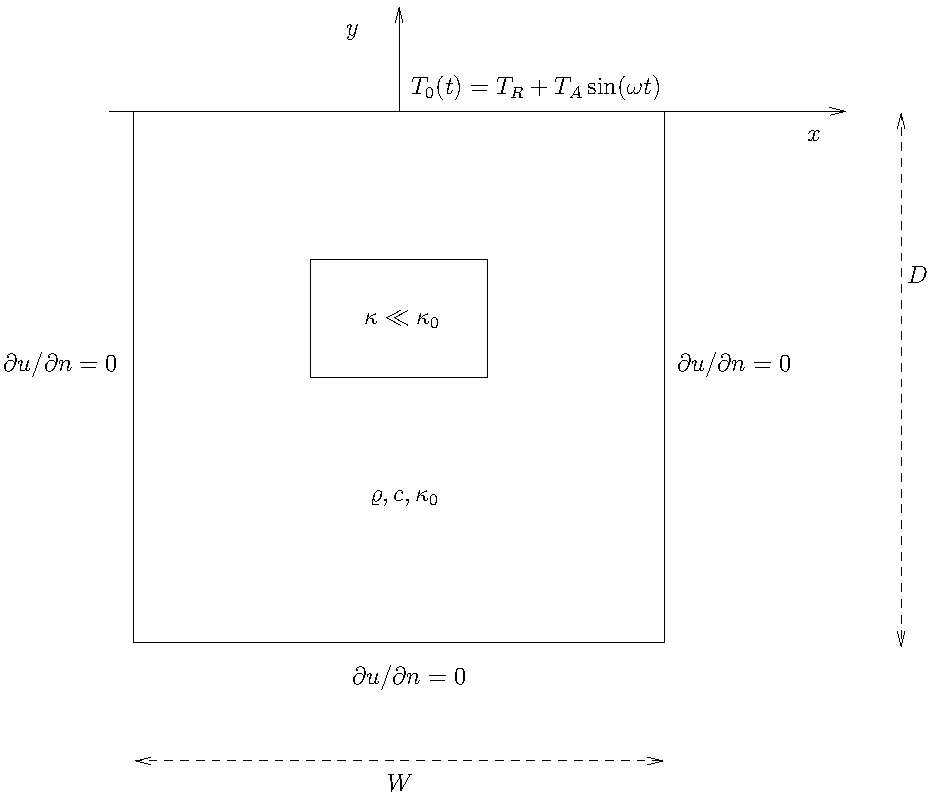
\includegraphics[width=0.8\linewidth]{chapters/langtangen/pdf/daynight.pdf}
    }
    \caption{
      Sketch of a (2D) problem involving heating and cooling of the ground due
      to an oscillating surface temperature.
    }
    \label{langtangen:timedep:diffusion2:sin:fig1}
  \end{center}
\end{figure}

The initial-boundary value problem for this problem reads
\begin{eqnarray}
\varrho c{\partial T\over\partial t} &=& \nabla\cdot\left( k\nabla T\right)\hbox{ in }\Omega\times (0,T],\\
T &=& T_0(t)\hbox{ on }\Gamma_0,\\
{\partial T\over\partial n} &=& 0\hbox{ on }\partial\Omega\cap\Gamma_0,\\
T &=& T_R\hbox{ at }t =0\langtangenep
\end{eqnarray}
Here, $\varrho$ is the density of the soil, $c$ is the
heat capacity, $\kappa$ is the thermal conductivity
(heat conduction coefficient)
in the soil, and $\Gamma_0$ is the surface boundary $x_{d-1}=0$.

We use a $\theta$-scheme in time, i.e., the evolution equation
$\partial P/\partial t=Q(t)$ is discretized as
\[ {P^k - P^{k-1}\over\Delta t} = \theta Q^k + (1-\theta )Q^{k-1},\]
where $\theta\in[0,1]$ is a weighting factor: $\theta =1$ corresponds
to the backward difference scheme, $\theta =1/2$ to the Crank-Nicolson
scheme, and $\theta =0$ to a forward difference scheme.
The $\theta$-scheme applied to our PDE results in
\[
\varrho c{T^k-T^{k-1}\over\Delta t} =
\theta \nabla\cdot\left( k\nabla T^k\right)
+ (1-\theta) \nabla\cdot\left( k\nabla T^{k-1}\right)\langtangenep
\]
Bringing this time-discrete PDE on weak form follows the technique shown
many times earlier in this tutorial. In the standard notation
$a(T,v)=L(v)$ the weak form has
\begin{eqnarray}
a(T,v) &=& \int_\Omega
\left( \varrho c Tv + \theta\Delta t \kappa\nabla v\cdot\nabla T\right)\dx,\\
L(v) &=& \int_\Omega \left( \varrho c vT^{k-1} - (1-\theta)\Delta t
\kappa\nabla v\cdot\nabla T\right)\dx\langtangenep
\end{eqnarray}
Observe that boundary integrals vanish because of the Neumann boundary
conditions.

The size of a 3D box is taken as $W\times W\times D$, where $D$ is
the depth and $W=D/2$ is the width.
We give the degree of the basis functions at the command line, then $D$,
and then the divisions of the domain in the various directions.
To make a box, rectangle, or interval of arbitrary (not unit) size,
we have the \dolfin{} classes {\fontsize{12pt}{12pt}\texttt{Box}}, {\fontsize{12pt}{12pt}\texttt{Rectangle}}, and
{\fontsize{12pt}{12pt}\texttt{Interval}} at our disposal. The mesh and the function space
can be created by the following code:
\begin{Verbatim}[fontsize=\fontsize{10pt}{10pt},tabsize=8,baselinestretch=1.05,
fontfamily=tt,xleftmargin=7mm]
degree = int(sys.argv[1])
D = float(sys.argv[2])
divisions = [int(arg) for arg in sys.argv[3:]]
d = len(divisions)  # no of space dimensions
if d == 1:
    mesh = Interval(divisions[0], -D, 0)
elif d == 2:
    mesh = Rectangle(0, -D, D/2, 0, divisions[0], divisions[1])
elif d == 3:
    mesh = Box(0, 0, -D, D/2, D/2, 0,
               divisions[0], divisions[1], divisions[2])
V = FunctionSpace(mesh, 'CG', degree)
\end{Verbatim}
\noindent
The {\fontsize{12pt}{12pt}\texttt{Rectangle}} and {\fontsize{12pt}{12pt}\texttt{Box}} instances are defined by the coordinates
of the ``minimum'' and ``maximum'' corners.

Setting Dirichlet conditions at the upper boundary can be done by
\begin{Verbatim}[fontsize=\fontsize{10pt}{10pt},tabsize=8,baselinestretch=1.05,
fontfamily=tt,xleftmargin=7mm]
T_R = 0; T_A = 1.0; omega = 2*pi
T_0 = Function(V, 'T_R + T_A*sin(omega*t)',
               {'T_R': T_R, 'T_A': T_A, 'omega': omega, 't': 0.0})

class Surface(SubDomain):
    def inside(self, x, on_boundary):
        return on_boundary and abs(x[d-1]) < 1E-14

surface = Surface()
bc = DirichletBC(V, T_0, surface)
\end{Verbatim}
\noindent
Quite simple values (non-physical for soil and real temperature variations)
are chosen for the initial testing.

The $\kappa$ function can be defined as a constant $\kappa_1$ inside
the particular rectangular area with a special soil composition, as
indicated in Figure~\ref{langtangen:timedep:diffusion2:sin:fig1}. Outside
this area $\kappa$ is a constant $\kappa_0$.
The domain of the rectangular area are taken as
\[ [-W/4, W/4]\times [-W/4, W/4]\times [-D/2, -D/2 + D/4]\]
in 3D, with $[-W/4, W/4]\times [-D/2, -D/2 + D/4]$ in 2D and
$[-D/2, -D/2 + D/4]$ in 1D.
Since we need some testing in the definition of the $\kappa(\langtangenxpoint)$
function, the most straightforward approach is to define a subclass
of {\fontsize{12pt}{12pt}\texttt{Function}}
with an {\fontsize{12pt}{12pt}\texttt{eval}} method for computing the values:
\begin{Verbatim}[fontsize=\fontsize{10pt}{10pt},tabsize=8,baselinestretch=1.05,
fontfamily=tt,xleftmargin=7mm]
class Kappa(Function):
    def eval(self, value, x):
        """x: spatial point, value[0]: function value."""
        d = len(x)  # no of space dimensions
        material = 0  # 0: outside, 1: inside
        if d == 1:
            if -D/2. < x[d-1] < -D/2. + D/4.:
                material = 1
        elif d == 2:
            if -D/2. < x[d-1] < -D/2. + D/4. and \
               -W/4. < x[0] < W/4.:
                material = 1
        elif d == 3:
            if -D/2. < x[d-1] < -D/2. + D/4. and \
               -W/4. < x[0] < W/4. and -W/4. < x[1] < W/4.:
                material = 1
        value[0] = kappa_0 if material == 0 else kappa_1
\end{Verbatim}
\noindent
The {\fontsize{12pt}{12pt}\texttt{eval}} method gives great flexibility in defining functions,
but a downside is that C++ calls up {\fontsize{12pt}{12pt}\texttt{eval}} in Python for
each point {\fontsize{12pt}{12pt}\texttt{x}}, which is a slow process, and the number of calls
is proportional to the number of nodes in the mesh.
Function expressions in terms of strings are compiled to efficient
C++ functions, being called from C++, so we should try to express functions
as string expressions if possible. (The {\fontsize{12pt}{12pt}\texttt{eval}} method can also be
defined through C++ code, but this is much
more involved and not covered here.)
Using inline if-tests in C++, we can make string expressions for
$\kappa$:
\begin{Verbatim}[fontsize=\fontsize{10pt}{10pt},tabsize=8,baselinestretch=1.05,
fontfamily=tt,xleftmargin=7mm]
kappa_0 = 0.2
kappa_1 = 0.001
kappa_str = {}
kappa_str[1] = 'x[0] > -%s/2 && x[0] < -%s/2 + %s/4 ? %g : %g' % \
               (D, D, D, kappa_1, kappa_0)
kappa_str[2] = 'x[0] > -%s/4 && x[0] < %s/4 '\
            '&& x[1] > -%s/2 && x[1] < -%s/2 + %s/4 ? %g : %g' % \
               (W, W, D, D, D, kappa_1, kappa_0)
kappa_str[3] = 'x[0] > -%s/4 && x[0] < %s/4 '\
               'x[1] > -%s/4 && x[1] < %s/4 '\
            '&& x[2] > -%s/2 && x[2] < -%s/2 + %s/4 ? %g : %g' % \
               (W, W, W, W, D, D, D, kappa_1, kappa_0)

kappa = Function(V, kappa_str[d])
\end{Verbatim}
\noindent
For example, in 2D {\fontsize{12pt}{12pt}\verb!kappa_str[1]!} becomes
\begin{Verbatim}[fontsize=\fontsize{10pt}{10pt},tabsize=8,baselinestretch=1.05,
fontfamily=tt,xleftmargin=7mm]
x[0] > -0.5/4 && x[0] < 0.5/4 && x[1] > -1.0/2 &&
x[1] < -1.0/2 + 1.0/4 ? 1e-07 : 0.2
\end{Verbatim}
\noindent
for $D=1$ and $W=D/2$ (the string is one line, but
broken into two here to fit the page width). It is very important to have
a {\fontsize{12pt}{12pt}\texttt{D}} that is {\fontsize{12pt}{12pt}\texttt{float}} and not {\fontsize{12pt}{12pt}\texttt{int}}, otherwise one gets
integer divisions in the C++ expression and a completely wrong $\kappa$
function.

We are now ready to define the initial condition and the
{\fontsize{12pt}{12pt}\texttt{a}} and {\fontsize{12pt}{12pt}\texttt{L}} forms of our problem:
\begin{Verbatim}[fontsize=\fontsize{10pt}{10pt},tabsize=8,baselinestretch=1.05,
fontfamily=tt,xleftmargin=7mm]
T_prev = interpolate(Constant(mesh, T_R), V)

rho = 1
c = 1
period = 2*pi/omega
T_stop = 5*period
dt = period/20  # 20 time steps per period
theta = 1

v = TestFunction(V)
T = TrialFunction(V)
f = Constant(mesh, 0)
a = rho*c*T*v*dx + theta*dt*kappa*dot(grad(v), grad(T))*dx
L = (rho*c*T_prev*v + dt*f*v -
     (1-theta)*dt*kappa*dot(grad(v), grad(T)))*dx

A = assemble(a)
b = None  # variable used for memory savings in assemble calls
\end{Verbatim}
\noindent
We could, alternatively, break {\fontsize{12pt}{12pt}\texttt{a}} and {\fontsize{12pt}{12pt}\texttt{L}} up in subexpressions
and assemble a mass matrix and stiffness matrix, as exemplified in
Chapter~\ref{langtangen:timedep:diffusion1:noassemble}, to avoid
assembly of {\fontsize{12pt}{12pt}\texttt{b}} at every time level. This modification is
straightforward and left as an exercise. The speed-up can be significant
in 3D problems.

The time loop is very similar to what we have displayed in
Chapter~\ref{langtangen:timedep:diffusion1:impl}:
\begin{Verbatim}[fontsize=\fontsize{10pt}{10pt},tabsize=8,baselinestretch=1.05,
fontfamily=tt,xleftmargin=7mm]
T = Function(V)   # unknown at the current time level
t = dt
while t <= T_stop:
    b = assemble(L, tensor=b)
    T_0.t = t
    bc.apply(A, b)
    solve(A, T.vector(), b)
    # visualization statements
    t += dt
    T_prev.assign(T)
\end{Verbatim}
\noindent
The complete code in {\fontsize{12pt}{12pt}\verb!diffusion123D_sin.py!} contains several
statements related to visualization of the solution, both as a
finite element field ({\fontsize{12pt}{12pt}\texttt{plot}} calls) and as a curve in the
vertical direction. The code also plots the exact analytical solution,
\[
T(x,t) = T_R + T_Ae^{ax}\sin (\omega t + ax),\quad a =\sqrt{\omega\varrho c\over 2\kappa},
\]
which is valid when $\kappa$ is constant throughout $\Omega$.
The reader is encouraged
to play around with the code and test out various parameter sets:
\begin{itemize}
\item $T_R=0$, $T_A=1$, $\kappa_0 = \kappa_1=0.2$, $\varrho = c = 1$, $\omega = 2\pi$
\item $T_R=0$, $T_A=1$, $\kappa_0=0.2$, $\kappa_1=0.01$, $\varrho = c = 1$, $\omega = 2\pi$
\item $T_R=0$, $T_A=1$, $\kappa_0=0.2$, $\kappa_1=0.001$, $\varrho = c = 1$, $\omega = 2\pi$
\item $T_R=10$ C, $T_A=10$ C, $\kappa_0= 1.1 \hbox{ K}^{-1}\hbox{Ns}^{-1}$,
$\kappa_0= 2.3 \hbox{ K}^{-1}\hbox{Ns}^{-1}$,
$\varrho = 1500\hbox{ kg/m}^3$,
$c = 1600\hbox{ Nm\,kg}^{-1}\hbox{K}^{-1}$,
$\omega = 2\pi/24$ 1/h  $= 7.27\cdot 10^{-5}$ 1/s, $D=1.5$ m
% kappa_1 = 1.1, varrho_1 = 1200, c_1 = 1000 => 9.17E-7
% kappa_0 = 2.3, varrho_0 = 1800, c_0 = 1500 => 8.52E-7
\end{itemize}
The latter set of data is relevant for real temperature variations in the
ground.


\section{Controlling the Solution of Linear Systems}
\label{langtangen:linsys}

Several linear algebra packages, referred to as
linear algebra \emph{backends}, can be used in \fenics{} to solve
linear systems:
PETSc, uBLAS, Epetra (Trilinos), or MTL4.
Which backend to apply can be controlled by setting
\begin{Verbatim}[fontsize=\fontsize{10pt}{10pt},tabsize=8,baselinestretch=1.05,
fontfamily=tt,xleftmargin=7mm]
parameters['linear algebra backend'] = backendname
\end{Verbatim}
\noindent
where {\fontsize{12pt}{12pt}\texttt{backendname}} is a string, either {\fontsize{12pt}{12pt}\texttt{'PETSc'}},
{\fontsize{12pt}{12pt}\texttt{'uBLAS'}}, {\fontsize{12pt}{12pt}\texttt{'Epetra'}}, or {\fontsize{12pt}{12pt}\texttt{'MTL4'}}.
These backends offer high-quality implementations of both iterative
and direct solvers for linear systems of equations.

The backend determines the specific data structures that are
used in the {\fontsize{12pt}{12pt}\texttt{Matrix}} and {\fontsize{12pt}{12pt}\texttt{Vector}} classes. For example,
with the PETSc backend, {\fontsize{12pt}{12pt}\texttt{Matrix}} encapsulates a
PETSc matrix storage structure, and
{\fontsize{12pt}{12pt}\texttt{Vector}} encapsulates a PETSc vector storage structure.
The underlying PETSc objects can be fetched by
\begin{Verbatim}[fontsize=\fontsize{10pt}{10pt},tabsize=8,baselinestretch=1.05,
fontfamily=tt,xleftmargin=7mm]
A_PETSc = down_cast(A).mat()
b_PETSc = down_cast(b).vec()
U_PETSc = down_cast(u.vector()).vec()
\end{Verbatim}
\noindent
Here, {\fontsize{12pt}{12pt}\texttt{u}} is a {\fontsize{12pt}{12pt}\texttt{Function}}, {\fontsize{12pt}{12pt}\texttt{A}} is a {\fontsize{12pt}{12pt}\texttt{Matrix}},
and {\fontsize{12pt}{12pt}\texttt{b}} is a {\fontsize{12pt}{12pt}\texttt{Vector}}.
The same syntax applies if we want to fetch
the underlying Epetra, uBLAS, or MTL4 matrices and vectors.

\subsection{Variational Problem Objects}

Let us explain how one can choose between direct and iterative solvers.
We have seen that there
are two ways of solving linear systems, either we call the {\fontsize{12pt}{12pt}\texttt{solve()}}
method in a {\fontsize{12pt}{12pt}\texttt{VariationalProblem}} instance or we call the {\fontsize{12pt}{12pt}\texttt{solve(A, U, b)}}
function with the assembled coefficient matrix {\fontsize{12pt}{12pt}\texttt{A}},
right-hand side vector {\fontsize{12pt}{12pt}\texttt{b}}, and
solution vector {\fontsize{12pt}{12pt}\texttt{U}}.

In case we use a {\fontsize{12pt}{12pt}\texttt{VariationalProblem}} instance, named {\fontsize{12pt}{12pt}\texttt{problem}},
it has a {\fontsize{12pt}{12pt}\texttt{parameters}} instance that behaves like a Python dictionary,
and we can use this object to choose between a direct or iterative
solver:
\begin{Verbatim}[fontsize=\fontsize{10pt}{10pt},tabsize=8,baselinestretch=1.05,
fontfamily=tt,xleftmargin=7mm]
problem.parameters['linear_solver'] = 'direct'
# or
problem.parameters['linear_solver'] = 'iterative'
\end{Verbatim}
\noindent
Another parameter {\fontsize{12pt}{12pt}\texttt{'symmetric'}} can be set to {\fontsize{12pt}{12pt}\texttt{True}}
if the coefficient matrix is symmetric so that
a method exploiting symmetry can be utilized.
For example, the default iterative solver is GMRES, but when solving
a Poisson equation, the iterative solution process will be more
efficient by setting the {\fontsize{12pt}{12pt}\texttt{'symmetry'}} parameter
so that a Conjugate Gradient is applied.

Having chosen an interative solver, we can invoke
a submenu {\fontsize{12pt}{12pt}\verb!'krylov_solver'!}
in the
{\fontsize{12pt}{12pt}\texttt{parameters}} object for setting various parameters for
the iterative solver (GMRES or Conjugate Gradients, depending on
whether the matrix is symmetric or not):
\begin{Verbatim}[fontsize=\fontsize{10pt}{10pt},tabsize=8,baselinestretch=1.05,
fontfamily=tt,xleftmargin=7mm]
itsolver = problem.parameters['krylov_solver'] # short form
itsolver['absolute_tolerance'] = 1E-10
itsolver['relative_tolerance'] = 1E-6
itsolver['divergence_limit'] = 1000.0
itsolver['gmres_restart'] = 50
itsolver['monitor_convergence'] = True
itsolver['report'] = True
\end{Verbatim}
\noindent
Here, {\fontsize{12pt}{12pt}\verb!'divergence_limit'!}
governs the maximum allowable number of iterations,
\hpl{why must it be a real and not an int?}
the {\fontsize{12pt}{12pt}\verb!'gmres_restart'!} parameter tells how many iterations GMRES performs before
it restarts,
{\fontsize{12pt}{12pt}\verb!'monitor_convergence'!} prints detailed information about the
development of the residual of a solver,
{\fontsize{12pt}{12pt}\verb!'report'!} governs whether a one-line report about the solution
method and the number of iterations
is written on the screen or not. The absolute and relative tolerances
enter (usually residual-based) stopping criteria, which are dependent on
the implementation of the underlying iterative solver in the actual backend.

\hpl{How are relative and absolute tolerances actually used?
Does it depend on the backend?}

When direct solver is chosen, there is similarly a submenu
{\fontsize{12pt}{12pt}\verb!'lu_solver'!} to set parameters, but here only the {\fontsize{12pt}{12pt}\texttt{'report'}}
parameter is available (since direct solvers very soldom have any
adjustable parameters). For nonlinear problems there is also
submenu {\fontsize{12pt}{12pt}\verb!'newton_solver'!} where tolerances, maximum iterations, and
so on, for a the Newton solver in {\fontsize{12pt}{12pt}\texttt{VariationalProblem}} can be set.

A complete list of all parameters and their default values
is printed to the screen by
\begin{Verbatim}[fontsize=\fontsize{10pt}{10pt},tabsize=8,baselinestretch=1.05,
fontfamily=tt,xleftmargin=7mm]
info(problem.parameters, True)
\end{Verbatim}
\noindent

\subsection{Solve Function}
\hpl{This will soon be outdated!}

For the {\fontsize{12pt}{12pt}\texttt{solve(A, x, b)}} approach, a 4th argument to {\fontsize{12pt}{12pt}\texttt{solve}}
determines the type of method:
\begin{itemize}
\item {\fontsize{12pt}{12pt}\texttt{'lu'}} for a sparse direct (LU decomposition) method,
\item {\fontsize{12pt}{12pt}\texttt{'cg'}} for the Conjugate Gradient (CG) method, which is
applicable if {\fontsize{12pt}{12pt}\texttt{A}} is symmetric and positive definite,
\item {\fontsize{12pt}{12pt}\texttt{'gmres'}} for
the GMRES iterative method, which is applicable when {\fontsize{12pt}{12pt}\texttt{A}} is nonsymmetric,
\item {\fontsize{12pt}{12pt}\texttt{'bicgstab'}} for
the BiCGStab iterative method, which is applicatble when {\fontsize{12pt}{12pt}\texttt{A}} is
nonsymmetric.
\end{itemize}
The default solver is {\fontsize{12pt}{12pt}\texttt{'lu'}}.

Good performance of an iterative method requires preconditioning of
the linear system. The 5th argument to {\fontsize{12pt}{12pt}\texttt{solve}} determines the
preconditioner:
\begin{itemize}
\item {\fontsize{12pt}{12pt}\texttt{'none'}} for no preconditioning.
\item {\fontsize{12pt}{12pt}\texttt{'jacobi'}} for the simple Jacobi (diagonal) preconditioner,
\item {\fontsize{12pt}{12pt}\texttt{'sor'}} for SOR preconditioning,
\item {\fontsize{12pt}{12pt}\texttt{'ilu'}} for incomplete LU factorization (ILU) preconditioning,
\item {\fontsize{12pt}{12pt}\texttt{'icc'}} for incomplete Cholesky factorization preconditioning
(requires {\fontsize{12pt}{12pt}\texttt{A}} to be symmetric and positive definite),
\item {\fontsize{12pt}{12pt}\verb!'amg_hypre'!} for algebraic multigrid (AMG) preconditioning
with the Hypre package (if available),
\item {\fontsize{12pt}{12pt}\verb!'mag_ml'!} for algebraic multigrid (AMG) preconditioning
with the ML package from Trilinos (if available),
\item {\fontsize{12pt}{12pt}\verb!'default_pc'!} for a default preconditioner, which depends
on the linear algebra backend ({\fontsize{12pt}{12pt}\texttt{'ilu'}} for PETSc).
%, a domain decomposition with ILU subdomain solver for Epetra).
\end{itemize}
If the 5th argument is not provided, {\fontsize{12pt}{12pt}\texttt{'ilu'}} is taken as the default
preconditioner.

Here are some sample calls to {\fontsize{12pt}{12pt}\texttt{solve}} demonstrating the choice
of solvers and preconditioners:
\begin{Verbatim}[fontsize=\fontsize{10pt}{10pt},tabsize=8,baselinestretch=1.05,
fontfamily=tt,xleftmargin=7mm]
solve(A, u.vector(), b)       # 'lu' is default solver
solve(A, u.vector(), cg)      # CG with ILU prec.
solve(A, u.vector(), 'gmres', 'amg_ml')  # GMRES with ML prec.
\end{Verbatim}
\noindent


\subsection{Setting the Start Vector}

The choice of start vector for the iterations in a linear solver is often
important. With the {\fontsize{12pt}{12pt}\texttt{solve(A, U, b)}} function the start vector
is the vector we feed in for the solution. A start vector
with random numbers in the interval $[-1,1]$ can be computed as
\begin{Verbatim}[fontsize=\fontsize{10pt}{10pt},tabsize=8,baselinestretch=1.05,
fontfamily=tt,xleftmargin=7mm]
n = u.vector().array().size
u.vector()[:] = numpy.random.uniform(-1, 1, n)
solve(A, u.vector(), b, cg, ilu)
\end{Verbatim}
\noindent
Or if a {\fontsize{12pt}{12pt}\texttt{VariationalProblem}} instance is used, its {\fontsize{12pt}{12pt}\texttt{solve}}
method may take an optional {\fontsize{12pt}{12pt}\texttt{u}} function as argument (which we
can fill with the right values):
\begin{Verbatim}[fontsize=\fontsize{10pt}{10pt},tabsize=8,baselinestretch=1.05,
fontfamily=tt,xleftmargin=7mm]
problem = VariationalProblem(a, L, bc)
n = u.vector().array().size
u.vector()[:] = numpy.random.uniform(-1, 1, n)
u = problem.solve(u)
\end{Verbatim}
\noindent

The program {\fontsize{12pt}{12pt}\verb!Poisson2D_DN_laprm.py!} demonstrates the various control mechanisms for
steering linear solvers as described above.

\subsection{Using a Backend-Specific Solver}

% ../../../la/trilinos/python/demo.py

Here is a demo where we operate on Trilinos-specific vectors, matrices,
iterative solvers, and preconditioners. Given a linear system
$AU=b$, represented by a {\fontsize{12pt}{12pt}\texttt{Matrix}} instance {\fontsize{12pt}{12pt}\texttt{A}},
and two {\fontsize{12pt}{12pt}\texttt{Vector}} instances {\fontsize{12pt}{12pt}\texttt{U}} and {\fontsize{12pt}{12pt}\texttt{b}}, the purpose is to
set up a solver using the Aztec Conjugate Gradient method from
Trilinos' Aztec library and combine that solver with the
algebraic multigrid preconditioner ML
from the ML library in Trilinos.
\begin{Verbatim}[fontsize=\fontsize{10pt}{10pt},tabsize=8,baselinestretch=1.05,
fontfamily=tt,xleftmargin=7mm]
try:
    from PyTrilinos import Epetra, AztecOO, TriUtils, ML
except:
    print '''You Need to have PyTrilinos with'
Epetra, AztecOO, TriUtils and ML installed
for this demo to run'''
    exit()

from dolfin import *

if not has_la_backend('Epetra'):
    print 'Warning: Dolfin is not compiled with Trilinos'
    exit()

parameters['linear_algebra_backend'] = 'Epetra'

# create matrix A and vector b in the usual way
# u is a Function

# Fetch underlying Epetra objects
A_epetra = down_cast(A).mat()
b_epetra = down_cast(b).vec()
U_epetra = down_cast(u.vector()).vec()

# Sets up the parameters for ML using a python dictionary
ML_param = {"max levels"        : 3,
            "output"            : 10,
            "smoother: type"    : "ML symmetric Gauss-Seidel",
            "aggregation: type" : "Uncoupled",
            "ML validate parameter list" : False
}

# Create the preconditioner
prec = ML.MultiLevelPreconditioner(A_epetra, False)
prec.SetParameterList(ML_param)
prec.ComputePreconditioner()

# Create solver and solve system
solver = AztecOO.AztecOO(A_epetra, U_epetra, b_epetra)
solver.SetPrecOperator(prec)
solver.SetAztecOption(AztecOO.AZ_solver, AztecOO.AZ_cg)
solver.SetAztecOption(AztecOO.AZ_output, 16)
solver.Iterate(MaxIters=1550, Tolerance=1e-5)

plot(u)
\end{Verbatim}
\noindent



\section{Creating More Complex Domains}
\label{langtangen:prepro}

Up to now we have been very fond of the unit square as domain,
which is an appropriate choice for initial versions of a
PDE solver. The strength of the finite element method, however, is its
ease of handling domains with complex shapes. This section
shows some methods that can be used to create different types of
domains and meshes.

Domains of complex shape must normally be constructed in separate
preprocessor programs. Two relevant preprocessors are Triangle for
2D domains and Netgen for 3D domains.

\subsection{Built-In Mesh Generation Tools}
\label{langtangen:prepro:builtin}

\dolfin{} has a few tools for creating various types of meshes over
domains with simple
shape:
{\fontsize{12pt}{12pt}\texttt{UnitInterval}},
{\fontsize{12pt}{12pt}\texttt{UnitSphere}},
{\fontsize{12pt}{12pt}\texttt{UnitSquare}},
{\fontsize{12pt}{12pt}\texttt{Interval}},
{\fontsize{12pt}{12pt}\texttt{Rectangle}},
{\fontsize{12pt}{12pt}\texttt{Box}},
{\fontsize{12pt}{12pt}\texttt{UnitCircle}},
and
{\fontsize{12pt}{12pt}\texttt{UnitCube}}.
Some of these names have been briefly met in previous sections.
The hopefully self-explanatory code snippet below summarizes
typical constructions of meshes with the aid of these tools:
\begin{Verbatim}[fontsize=\fontsize{10pt}{10pt},tabsize=8,baselinestretch=1.05,
fontfamily=tt,xleftmargin=7mm]
# 1D domains
mesh = UnitInterval(20)     # 20 cells, 21 vertices
mesh = Interval(20, -1, 1)  # domain [-1,1]

# 2D domains (6x10 divisions, 120 cells, 77 vertices)
mesh = UnitSquare(6, 10)  # 'right' diagonal is default
# The diagonals can be right, left or crossed
mesh = UnitSquare(6, 10, 'left')
mesh = UnitSquare(6, 10, 'crossed')

# Domain [0,3]x[0,2] with 6x10 divisions and left diagonals
mesh = Rectangle(0, 0, 3, 2, 6, 10, 'left')

# 6x10x5 boxes in the unit cube, each box gets 6 tetrahedra:
mesh = UnitCube(6, 10, 5)

# Domain [-1,1]x[-1,0]x[-1,2] with 6x10x5 divisions
mesh = Box(-1, -1, -1, 1, 0, 2, 6, 10, 5)

# 10 divisions in radial directions
mesh = UnitCircle(10)
mesh = UnitSphere(10)
\end{Verbatim}
\noindent

\subsection{Transforming Mesh Coordinates}
\label{langtangen:mesh:transform:cyl}

A mesh that is denser toward a boundary is often desired to increase
accuracy in that region. Given a mesh with uniformly spaced
coordinates $x_0,\ldots,x_{M-1}$ in $[a,b]$, the coordinate transformation
$\xi = (x-a)/(b-a)$ maps $x$ onto $\xi\in [0,1]$. A new mapping
$\eta = \xi^s$, for some $s>1$, stretches the mesh toward $\xi=0$ ($x=a$),
while $\eta = \xi^{1/s}$ makes a stretching toward $\xi=1$ ($x=b$).
Mapping the $\eta\in[0,1]$ coordinates back to $[a,b]$ gives new,
stretched $x$ coordinates,
\begin{equation}
\bar x = a + (b-a)\left({x-a\over b-a}\right)^s
\end{equation}
toward $x=a$, or
\begin{equation}
\bar x = a + (b-a)\left({x-a\over b-a}\right)^{1/s}
\end{equation}
toward $x=b$

One way of creating more complex geometries is to transform the
vertex coordinates in a rectangular mesh according to some formula.
Say we want to create a part of a hollow cylinder of $\Theta$ degrees,
with inner radius $a$ and outer radius $b$. A standard mapping from polar
coordinates to Cartesian coordinates can be used to generate the
hollow cylinder. Given a rectangle in $(\bar x, \bar y)$ space such that
$a\leq \bar x\leq b$ and $0\leq \bar y\leq 1$, the mapping
\[ \hat x = \bar x\cos (\Theta \bar y),\quad \hat y = \bar x\sin (\Theta \bar y),\]
takes a point in the rectangular $(\bar x,\bar y)$
geometry and maps it to a point
$(\hat x, \hat y)$ in a hollow cylinder.

The corresponding Python code for first stretching the mesh and
then mapping it onto a hollow cylinder looks as follows:
\begin{Verbatim}[fontsize=\fontsize{10pt}{10pt},tabsize=8,baselinestretch=1.05,
fontfamily=tt,xleftmargin=7mm]
Theta = pi/2
a, b = 1, 5.0
nr = 10  # divisions in r direction
nt = 20  # divisions in theta direction
mesh = Rectangle(a, 0, b, 1, nr, nt, 'crossed')

# First make a denser mesh towards r=a
x = mesh.coordinates()[:,0]
y = mesh.coordinates()[:,1]
s = 1.3

def denser(x, y):
    return [a + (b-a)*((x-a)/(b-a))**s, y]

x_bar, y_bar = denser(x, y)
xy_bar_coor = numpy.array([x_bar, y_bar]).transpose()
mesh.coordinates()[:] = xy_bar_coor
plot(mesh, title='stretched mesh')

def cylinder(r, s):
    return [r*cos(Theta*s), r*sin(Theta*s)]

x_hat, y_hat = cylinder(x_bar, y_bar)
xy_hat_coor = numpy.array([x_hat, y_hat]).transpose()
mesh.coordinates()[:] = xy_hat_coor
plot(mesh, title='hollow cylinder')
interactive()
\end{Verbatim}
\noindent
The result of calling {\fontsize{12pt}{12pt}\texttt{denser}} and {\fontsize{12pt}{12pt}\texttt{cylinder}} above is a list of two
vectors, with the $x$ and $y$ coordinates, respectively.
Turning this list into a {\fontsize{12pt}{12pt}\texttt{numpy}} array object results in a $2\times M$
array, $M$ being the number of vertices in the mesh. However,
{\fontsize{12pt}{12pt}\texttt{mesh.coordinates()}} is by convention an $M\times 2$ array so we
need to take the transpose. The resulting mesh is displayed
in Figure~\ref{langtangen:mesh:transform:cyl:fig1}.
\begin{figure}
  \begin{center}
    \centerline{
      {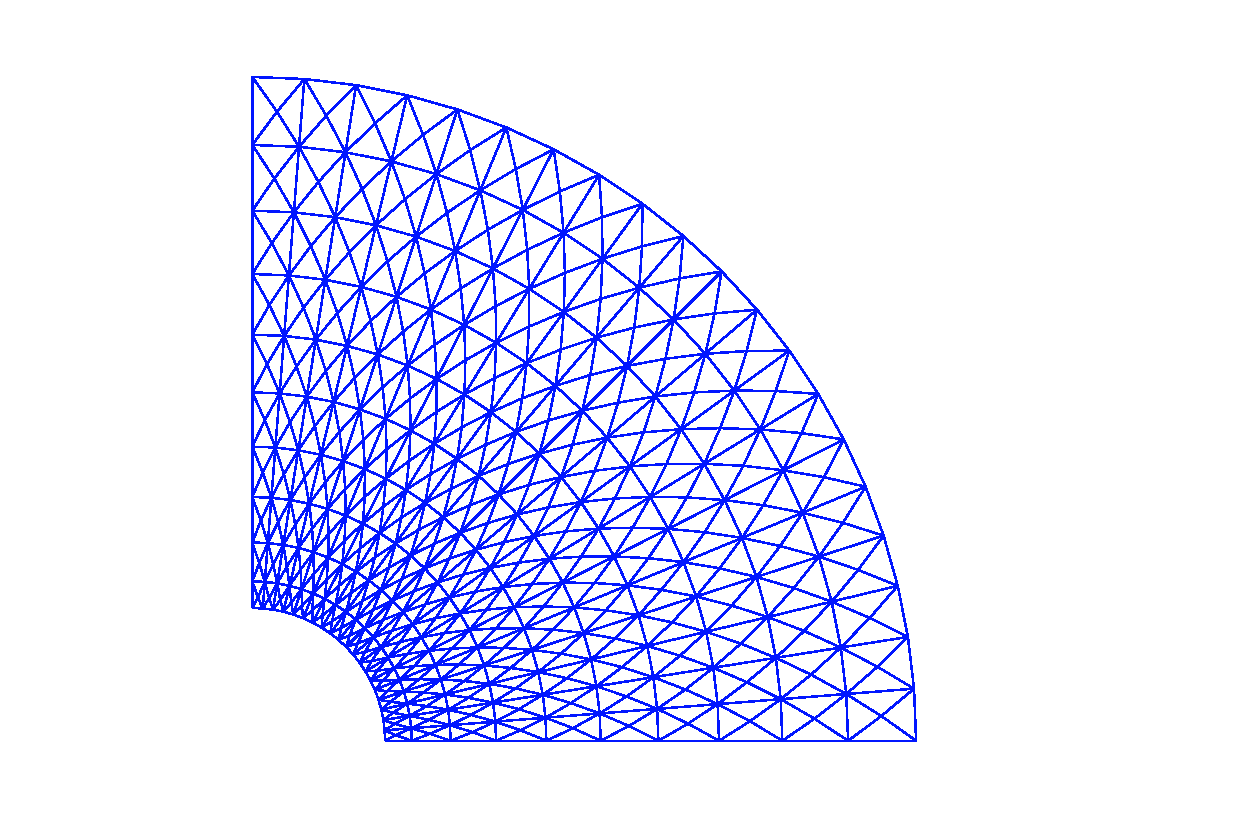
\includegraphics[width=0.9\linewidth]{chapters/langtangen/pdf/hollow_cylinder.pdf}}}
    \caption{Hollow cylinder generated by mapping a rectangular mesh, stretched toward
      the left side.}
    \label{langtangen:mesh:transform:cyl:fig1}
  \end{center}
\end{figure}


%Stretch coordinates according to Mikael.
%Use refine uniformly and adaptively (adaptive poisson demo, use just
%grad u for example)
%Check ../../dielectric/python/demo.py og MeshEditor!
%Use refine og move.
%
%CHeck Netgen examples in the source, 2D.

%Transfinite mappings? Laplace?

\subsection{Separate Preprocessor Applications}

\section{Handling Domains with Different Materials}

Solving PDEs in domains made up of different materials is a frequently
encountered task. In \fenics, this kind of problems are handled by
defining subdomains inside the domain. The subdomains may represent the
various materials. We can thereafter define material properties through
functions, known in \fenics{} as \emph{mesh functions},
that are piecewise constant in each subdomain.
A simple example with
two materials (subdomains) in 2D will
demonstrate the basic steps in the process. Later, a multi-material
problem in $d$ space dimensions is addressed.

\subsection{Working with Two Subdomains}
\label{langtangen:possion:2D:2mat:problem}


Suppose we want to solve
\begin{equation} \label{langtangen:poisson:2D:2mat:varcoeff2}
    \nabla\cdot \left\lbrack k(x,y)\nabla u(x,y)\right\rbrack = 0,
\end{equation}
in a domain $\Omega$ consisting of two subdomains where $k$ takes on
a different value in each subdomain.
For simplicity, yet without loss of generality, we choose for the current
implementation
the domain $\Omega = [0,1]\times [0,1]$ and divide it into two equal
subdomains, as depicted in Figure~\ref{langtangen:possion:2D:2mat:fig1},
\[ \Omega_0 = [0, 1]\times [0,1/2],\quad
\Omega_1 = [0, 1]\times (1/2,1]\langtangenep\]
We define $k(x,y)=1$ in $\Omega_0$ and $k(x,y)=10$ in $\Omega_1$.
As boundary conditions, we choose $u=0$ at $x=0$, $u=1$ at $x=1$,
and $\partial u/\partial n=0$ at $y=0$ and $y=1$.
This choice implies the simple solution $u(x,y)=x$, which we should
recover exactly with linear or higher order finite elements.

\begin{figure}
  \begin{center}
    % NOTE: remove everything with \SetFigFont etc from xfig
    \newcommand{\SetFigFontNFSS}[2]{}
    \centerline{
      %\setlength{\unitlength}{4144sp}
      \setlength{\unitlength}{2144sp}
      % no blank line before begin{picture}
      \begin{picture}(6372,6030)(166,-6376)
        \thinlines
            {\color[rgb]{0,0,0}\put(901,-5956){\vector( 0, 1){5445}}
            }%
            {\color[rgb]{0,0,0}\put(901,-5911){\vector( 1, 0){5625}}
            }%
            {\color[rgb]{0,0,0}\put(901,-2086){\line( 1, 0){3825}}
              \put(4726,-2086){\line( 0,-1){3825}}
            }%
            {\color[rgb]{0,0,0}\put(901,-4021){\line( 1, 0){3825}}
            }%
            \put(6301,-6226){$x$}
            \put(586,-601){$y$}
            %\put(2251,-6361){$\partial u/\partial n=0$}
            %\put(2251,-1861){$\partial u/\partial n=0$}
            \put(2300,-6361){$\partial u/\partial n=0$}
            \put(2300,-1861){$\partial u/\partial n=0$}
            %\put(2431,-3211){$\Omega_1$}
            %\put(2476,-5191){$\Omega_0$}
            \put(2700,-3211){$\Omega_1$}
            \put(2700,-5050){$\Omega_0$}
            %\put(181,-4156){$u=0$}
            \put(151,-4111){$u=0$}
            \put(4861,-4111){$u=1$}
      \end{picture}%
    }
    \caption{Sketch of a Poisson problem with a variable coefficient that is constant
      in each of the two subdomains $\Omega_0$ and $\Omega_1$.
    }
    \label{langtangen:possion:2D:2mat:fig1}
  \end{center}
\end{figure}

Physically, the present problem may correspond to heat conduction, where
the heat conduction in $\Omega_1$ is ten times more efficient than
in $\Omega_0$. An alternative interpretation is flow in porous media
with two geological layers, where the layers' ability to transport
the fluid differs by a factor of 10.

\subsection{The Implementation}
\label{langtangen:possion:2D:2mat:impl}


The new functionality in this subsection regards how to
to define the subdomains
$\Omega_0$ and $\Omega_1$. Defining a subdomain is done by
creating a subclass of {\fontsize{12pt}{12pt}\texttt{SubDomain}} and implementing the
{\fontsize{12pt}{12pt}\texttt{inside}} function. In the present case we define
\begin{Verbatim}[fontsize=\fontsize{10pt}{10pt},tabsize=8,baselinestretch=1.05,
fontfamily=tt,xleftmargin=7mm]
class Omega0(SubDomain):
    def inside(self, x, on_boundary):
        return True if x[1] <= 0.5 else False

class Omega1(SubDomain):
    def inside(self, x, on_boundary):
        return True if x[1] >= 0.5 else False
\end{Verbatim}
\noindent

The next task is to introduce a {\fontsize{12pt}{12pt}\texttt{MeshFunction}} to mark all
cells in $\Omega_0$ with the subdomain number 0 and all cells in $\Omega_1$
with the subdomain number 1.
Our convention is to number subdomains as $0,1,2,\ldots$.

A {\fontsize{12pt}{12pt}\texttt{MeshFunction}} is a discrete function that can be evaluated at a set
of so-called \emph{mesh entities}. Three mesh entities are
cells, facets, and vertices. A {\fontsize{12pt}{12pt}\texttt{MeshFunction}} over cells is suitable to
represent subdomains (materials), while a {\fontsize{12pt}{12pt}\texttt{MeshFunction}} over
facets is used to represent pieces of external or internal boundaries.
Mesh functions over vertices can be used to describe continuous fields.

Since we need to define subdomains of $\Omega$
in the present example, we must make use
of a {\fontsize{12pt}{12pt}\texttt{MeshFunction}} over cells. The
{\fontsize{12pt}{12pt}\texttt{MeshFunction}} constructor is fed with three arguments: 1) the type
of value: {\fontsize{12pt}{12pt}\texttt{'int'}} for integers, {\fontsize{12pt}{12pt}\texttt{'uint'}} for positive
(unsigned) integers, {\fontsize{12pt}{12pt}\texttt{'double'}} for real numbers, and
{\fontsize{12pt}{12pt}\texttt{'bool'}} for logical values; 2) a {\fontsize{12pt}{12pt}\texttt{Mesh}} instance, and 3)
the topological dimension of the mesh entity in question: cells
have topological dimension equal to the number of space dimensions in
the PDE problem, and facets have one dimension lower.
Alternatively, the constructor can take just a filename
and initialize the {\fontsize{12pt}{12pt}\texttt{MeshFunction}} from data in a file. We shall
demonstrate this functionality in the next multi-material problem
in Chapter~\ref{langtangen:possion:nD:nmat}.

We start with creating a {\fontsize{12pt}{12pt}\texttt{MeshFunction}} whose
values are non-negative integers ({\fontsize{12pt}{12pt}\texttt{'uint'}})
for numbering the subdomains.
The mesh entities of interest are the cells, which have dimension 2
in a two-dimensional problem (1 in 1D, 3 in 3D). The appropriate code for
defining the {\fontsize{12pt}{12pt}\texttt{MeshFunction}} for two subdomains then reads
\begin{Verbatim}[fontsize=\fontsize{10pt}{10pt},tabsize=8,baselinestretch=1.05,
fontfamily=tt,xleftmargin=7mm]
subdomains = MeshFunction('uint', mesh, 2)
# Mark subdomains with numbers 0 and 1
subdomain0 = Omega0()
subdomain0.mark(subdomains, 0)
subdomain1 = Omega1()
subdomain1.mark(subdomains, 1)
\end{Verbatim}
\noindent

Calling {\fontsize{12pt}{12pt}\texttt{subdomains.values()}} returns a {\fontsize{12pt}{12pt}\texttt{numpy}} array of the
subdomain values. That is, {\fontsize{12pt}{12pt}\texttt{subdomain.values()[i]}} is
the subdomain value of cell no.~{\fontsize{12pt}{12pt}\texttt{i}}. This array is used to
look up the subdomain or material number of a specific element.

Now we want a function {\fontsize{12pt}{12pt}\texttt{k}} that is piecewise constant in
each subdomain $\Omega_0$ and $\Omega_1$. Since we want {\fontsize{12pt}{12pt}\texttt{k}}
to be a finite element function, it is natural to choose
a space of functions that are constant over each element.
The family of discontinuous Galerkin methods, in \fenics{}
denoted by {\fontsize{12pt}{12pt}\texttt{'DG'}}, is suitable for this purpose. Since we
want functions that are piecewise constant, the value of
the degree parameter is zero:
\begin{Verbatim}[fontsize=\fontsize{10pt}{10pt},tabsize=8,baselinestretch=1.05,
fontfamily=tt,xleftmargin=7mm]
V0 = FunctionSpace(mesh, 'DG', 0)
k  = Function(V0)
\end{Verbatim}
\noindent
To fill {\fontsize{12pt}{12pt}\texttt{k}} with the right values in each element, we loop over
all cells (i.e., indices in {\fontsize{12pt}{12pt}\texttt{subdomain.values()}}),
extract the corresponding subdomain number of a cell,
and assign the corresponding $k$ value to the {\fontsize{12pt}{12pt}\texttt{k.vector()}} array:
\begin{Verbatim}[fontsize=\fontsize{10pt}{10pt},tabsize=8,baselinestretch=1.05,
fontfamily=tt,xleftmargin=7mm]
k_values = [1.5, 50]  # values of k in the two subdomains
for cell_no in range(len(subdomains.values())):
    subdomain_no = subdomains.values()[cell_no]
    k.vector()[cell_no] = k_values[subdomain_no]
\end{Verbatim}
\noindent

Long loops in Python are known to be slow, so for large meshes the
it is preferable to avoid such loops and instead use \emph{vectorized code}.
Normally this implies that the loop must be replaced by
calls to functions from the {\fontsize{12pt}{12pt}\texttt{numpy}} library that operate on complete
arrays (in efficient C code). The functionality we want in the present
case is to compute an array of the same size as
{\fontsize{12pt}{12pt}\verb!subdomain.values()!}, but where the value {\fontsize{12pt}{12pt}\texttt{i}} of an entry
in {\fontsize{12pt}{12pt}\verb!subdomain.values()!} is replaced by {\fontsize{12pt}{12pt}\verb!k_values[i]!}.
Such an operation is carried out by the {\fontsize{12pt}{12pt}\texttt{numpy}} function {\fontsize{12pt}{12pt}\texttt{choose}}:
\begin{Verbatim}[fontsize=\fontsize{10pt}{10pt},tabsize=8,baselinestretch=1.05,
fontfamily=tt,xleftmargin=7mm]
help = numpy.asarray(subdomains.values(), dtype=numpy.int32)
k.vector()[:] = numpy.choose(help, k_values)
\end{Verbatim}
\noindent
The {\fontsize{12pt}{12pt}\texttt{help}} array is required since {\fontsize{12pt}{12pt}\texttt{choose}} cannot work with
{\fontsize{12pt}{12pt}\verb!subdomain.values()!} because this array has elements of
type {\fontsize{12pt}{12pt}\texttt{uint32}}. We must therefore transform this array to an array
{\fontsize{12pt}{12pt}\texttt{help}} with standard {\fontsize{12pt}{12pt}\texttt{int32}} integers.

Having the {\fontsize{12pt}{12pt}\texttt{k}} function ready for finite element computations, we
can proceed in the normal manner with defining essential boundary
conditions, as in Chapter~\ref{langtangen:poisson:multiple:Dirichlet},
and the $a(u,v)$ and $L(v)$ forms, as in
Chapter~\ref{langtangen:possion:2D:varcoeff}.
All the details can be found in the file {\fontsize{12pt}{12pt}\verb!Poisson2D_2mat.py!}.


\subsection{Multiple Neumann, Robin, and Dirichlet Conditions}
\label{langtangen:poisson:mat:neumann}

Let us go back to the model problem from
Chapter~\ref{langtangen:poisson:multiple:Dirichlet}
where we had both Dirichlet and Neumann conditions.
The term {\fontsize{12pt}{12pt}\texttt{v*g*ds}} in the expression for {\fontsize{12pt}{12pt}\texttt{L}} implies a
boundary integral over the complete boundary, or in \fenics{} terms,
an integral over all exterior cell facets.
However, the contributions from the parts of the boundary where we have
Dirichlet conditions are erased when the linear system is modified by
the Dirichlet conditions.
We would like, from an efficiency point of view, to integrate {\fontsize{12pt}{12pt}\texttt{v*g*ds}}
only over the parts of the boundary where we actually have Neumann conditions.
And more importantly,
in other problems one may have different Neumann conditions or
other conditions like the Robin type condition.
With the mesh function concept we can mark
different parts of the boundary and integrate over specific parts.
The same concept can also be used to treat multiple Dirichlet conditions.
The forthcoming text illustrates how this is done.

Essentially, we still stick to the model problem from
Chapter~\ref{langtangen:poisson:multiple:Dirichlet}, but replace the
Neumann condition at $y=0$ by a \emph{Robin condition}\footnote{The Robin condition is
most often used to model heat transfer to the surroundings and arise
naturally from Newton's cooling law.}:
\[ -{\partial u\over\partial n} = p(u-q),\]
where $p$ and $q$ are specified functions.
Since we have prescribed a simple solution in our model problem,
$u=1+x^2+y^4$, we adjust $p$ and $q$ such that the condition holds
at $y=0$. This implies that $q=1+x^2+2y^2$ and $p$ can be arbitrary
(the normal derivative at $y=0$: $\partial u/\partial n = -\partial u/\partial y = -4y=0$).

Now we have four parts of the boundary: $\Gamma_N$ which corresponds to
the upper side $y=1$, $\Gamma_R$ which corresponds to the lower part
$y=0$, $\Gamma_0$ which corresponds to the left part $x=0$, and
$\Gamma_1$ which corresponds to the right part $x=1$. The
complete boundary-value problem reads
\begin{eqnarray}
    - \Delta u &=& -6 \mbox{ in } \Omega, \label{langtangen:poisson:2D:DN3}\\
    u &=& u_L \mbox{ on } \Gamma_0, \label{langtangen:poisson:2D:DN3:bc1}\\
    u &=& u_R \mbox{ on } \Gamma_1, \label{langtangen:poisson:2D:DN3:bc2}\\
    - {\partial u\over\partial n} &=& p(u-q) \mbox{ on } \Gamma_R,
    \label{langtangen:poisson:2D:DN3:bc3}\\
    - {\partial u\over\partial n} &=& 4y \mbox{ on } \Gamma_N\langtangenep
    \label{langtangen:poisson:2D:DN3:bc4}
\end{eqnarray}
The involved prescribed functions are $u_L== 1 + 2y^2$,
$u_R = 2 + 2y^2$, $q=1+x^2+2y^2$, $p$ is arbitrary, and $g=-4y$.

Integration by parts of $-\int_\Omega v\Delta u\dx$ becomes
as usual
\[
 -\int_\Omega v\Delta u \dx
= \int_\Omega\nabla v\cdot\nabla u\dx - \int_{\partial\Omega}v{\partial u\over
\partial n}\ds\langtangenep
\]
The boundary integral vanishes on $\Gamma_0\cup\Gamma_1$, and
we split the parts over $\Gamma_N$ and $\Gamma_R$ since we have
different conditions at those parts:
\[
- \int_{\partial\Omega}v{\partial u\over
\partial n}\ds
=
-\int_{\Gamma_N}v{\partial u\over
\partial n}\ds -
\int_{\Gamma_R}v{\partial u\over
\partial n}\ds
= \int_{\Gamma_N}vg\ds +
\int_{\Gamma_R}vp(u-q)\ds\langtangenep
\]
The weak form then becomes
\[
\int_{\Omega} \nabla v \cdot \nabla u \dx +
\int_{\Gamma_N} g v\ds + \int_{\Gamma_R}vp(u-q)\ds
= \int_{\Omega} fv \dx,
\]
We want to write this weak form in the standard
notation $a(u,v)=L(v)$, which
requires that we indentify all integrals with \emph{both} $u$ and $v$,
and collect these in $a(u,v)$, while the remaining integrals with
$v$ and not $u$ go
into $L(v)$.
The integral from the Robin condition must of this reason be split in two
parts:
\[ \int_{\Gamma_R}vp(u-q)\ds
= \int_{\Gamma_R}vpu\ds - \int_{\Gamma_R}vpq\ds\langtangenep
\]
We then have
\begin{eqnarray}
a(u, v) &=& \int_{\Omega} \nabla v \cdot \nabla u \dx
+ \int_{\Gamma_R}vpu\ds,
\label{langtangen:poisson:2D:DN3:var:a}\\
L(v) &=& \int_{\Omega} fv \dx -
\int_{\Gamma_N} g v\ds + \int_{\Gamma_R}vpq\ds\langtangenep
\label{langtangen:poisson:2D:DN3:var:L}
\end{eqnarray}

A natural starting point for implementation is
the {\fontsize{12pt}{12pt}\verb!Poisson2D_DN2.py!} program, which we now copy to
{\fontsize{12pt}{12pt}\verb!Poisson2D_DNR.py!}.
The new aspects are
\begin{enumerate}
\item definition of a mesh function over the boundary,
\item marking each side as a subdomain, using the mesh function,
\item splitting a boundary integral into parts.
\end{enumerate}

Task 1 makes use of the {\fontsize{12pt}{12pt}\texttt{MeshFunction}} object, but contrary to
Chapter~\ref{langtangen:possion:2D:2mat:impl}, this is not a function over
cells, but a function over cell facets. The topological dimension of
cell facets is one lower than the cell interiors, so in a two-dimensional
problem the dimension
becomes 1. In general, the facet dimension
is given as {\fontsize{12pt}{12pt}\texttt{mesh.topology().dim()-1}},
which we use in the code for ease of direct reuse in other problems.
The construction of a {\fontsize{12pt}{12pt}\texttt{MeshFunction}} instance to mark boundary parts
now reads
\begin{Verbatim}[fontsize=\fontsize{10pt}{10pt},tabsize=8,baselinestretch=1.05,
fontfamily=tt,xleftmargin=7mm]
boundary_parts = \
  MeshFunction("uint", mesh, mesh.topology().dim()-1)
\end{Verbatim}
\noindent
As in Chapter~\ref{langtangen:possion:2D:2mat:impl} we
use a subclass of {\fontsize{12pt}{12pt}\texttt{SubDomain}} to identify the various parts
of the mesh function. Problems with domains of more complicated may
set the mesh function for marking boundaries as part of the mesh
generation.
In our case, the $y=0$ boundary can be marked by
\begin{Verbatim}[fontsize=\fontsize{10pt}{10pt},tabsize=8,baselinestretch=1.05,
fontfamily=tt,xleftmargin=7mm]
class LowerRobinBoundary(SubDomain):
    def inside(self, x, on_boundary):
        tol = 1E-14   # tolerance for coordinate comparisons
        return on_boundary and abs(x[1]) < tol

Gamma_R = LowerRobinBoundary()
Gamma_R.mark(boundary_parts, 0)
\end{Verbatim}
\noindent
The code for the $y=1$ boundary is similar and is seen in
{\fontsize{12pt}{12pt}\verb!Poisson2D_DNR.py!}.

The Dirichlet boundaries are marked similarly, using subdomain number 2 for $\Gamma_0$ and 3 for $\Gamma_1$:
\begin{Verbatim}[fontsize=\fontsize{10pt}{10pt},tabsize=8,baselinestretch=1.05,
fontfamily=tt,xleftmargin=7mm]
class LeftDirichletBoundary(SubDomain):
    def inside(self, x, on_boundary):
        tol = 1E-14   # tolerance for coordinate comparisons
        return on_boundary and abs(x[0]) < tol

Gamma_0 = LeftDirichletBoundary()
Gamma_0.mark(boundary_parts, 2)

class RightDirichletBoundary(SubDomain):
    def inside(self, x, on_boundary):
        tol = 1E-14   # tolerance for coordinate comparisons
        return on_boundary and abs(x[0] - 1) < tol

Gamma_1 = RightDirichletBoundary()
Gamma_1.mark(boundary_parts, 3)
\end{Verbatim}
\noindent
Specifying the {\fontsize{12pt}{12pt}\texttt{DirichletBC}} instances may now make use of
the mesh function (instead of a {\fontsize{12pt}{12pt}\texttt{SubDomain}} subclass object)
and an indicator for which subdomain each condition
should be applied to:
\begin{Verbatim}[fontsize=\fontsize{10pt}{10pt},tabsize=8,baselinestretch=1.05,
fontfamily=tt,xleftmargin=7mm]
u_L = Function(V, '1 + 2*x[1]*x[1]')
u_R = Function(V, '2 + 2*x[1]*x[1]')
bc = [DirichletBC(V, u_L, boundary_parts, 2),
      DirichletBC(V, u_R, boundary_parts, 3)]
\end{Verbatim}
\noindent

Some functions need to be defined before we can go on with the
{\fontsize{12pt}{12pt}\texttt{a}} and {\fontsize{12pt}{12pt}\texttt{L}} of the variational problem:
\begin{Verbatim}[fontsize=\fontsize{10pt}{10pt},tabsize=8,baselinestretch=1.05,
fontfamily=tt,xleftmargin=7mm]
q = Function(V, '1 + x[0]*x[0] + 2*x[1]*x[1]')
p = Constant(mesh, 100)  # arbitrary function can go here
v = TestFunction(V)
u = TrialFunction(V)
f = Constant(mesh, -6.0)
\end{Verbatim}
\noindent

The new aspect of the variational problem is the two distinct
boundary integrals.
Having a mesh function over exterior cell facets (i.e., our
{\fontsize{12pt}{12pt}\verb!boundary_parts!} object), where subdomains (boundary parts) are
numbered as $0,1,2,\ldots$, the special symbol {\fontsize{12pt}{12pt}\texttt{ds(0)}}
implies integration over subdomain (part) 0, {\fontsize{12pt}{12pt}\texttt{ds(1)}} denotes
integration over subdomain (part) 1, and so on.
The idea of multiple {\fontsize{12pt}{12pt}\texttt{ds}}-type objects generalizes to volume
integrals too: {\fontsize{12pt}{12pt}\texttt{dx(0)}}, {\fontsize{12pt}{12pt}\texttt{dx(1)}}, etc., are used to
integrate over subdomain 0, 1, etc.,  inside $\Omega$.

The variational problem can be defined as
\begin{Verbatim}[fontsize=\fontsize{10pt}{10pt},tabsize=8,baselinestretch=1.05,
fontfamily=tt,xleftmargin=7mm]
a = dot(grad(v), grad(u))*dx + v*p*u*ds(0)
L = v*f*dx - v*g*ds(1) + v*p*q*ds(0)
\end{Verbatim}
\noindent
For the {\fontsize{12pt}{12pt}\texttt{ds(0)}} and {\fontsize{12pt}{12pt}\texttt{ds(1)}} symbols to work we must obviously
connect them (or {\fontsize{12pt}{12pt}\texttt{a}} and {\fontsize{12pt}{12pt}\texttt{L}}) to the mesh function marking
parts of the boundary. This is done by a certain keyword argument
to the {\fontsize{12pt}{12pt}\texttt{assemble}} function:
\begin{Verbatim}[fontsize=\fontsize{10pt}{10pt},tabsize=8,baselinestretch=1.05,
fontfamily=tt,xleftmargin=7mm]
A = assemble(a, exterior_facet_domains=boundary_parts)
b = assemble(L, exterior_facet_domains=boundary_parts)
\end{Verbatim}
\noindent
Then essential boundary conditions are enforced, and the system can
be solved in the usual way:
\begin{Verbatim}[fontsize=\fontsize{10pt}{10pt},tabsize=8,baselinestretch=1.05,
fontfamily=tt,xleftmargin=7mm]
for condition in bc: condition.apply(A, b)
u = Function(V)
solve(A, u.vector(), b)
\end{Verbatim}
\noindent

At the time of this writing, it is not possible to perform integrals over
different parts of the domain or boundary using the
{\fontsize{12pt}{12pt}\verb!assemble_system!} function or the
{\fontsize{12pt}{12pt}\texttt{VariationalProblem}} instance.


\section{A General $d$-Dimensional Multi-Material Test Problem}
\label{langtangen:possion:nD:nmat}

{\bf This section is in a preliminary state!}

The purpose of the present section is to generalize the basic
ideas from the previous section to a problem involving
an arbitrary number of materials in 1D, 2D, or 3D domains.
The example also highlights how to build more general and flexible
\fenics{} applications.

\subsection{The PDE Problem}
\label{langtangen:possion:nD:nmat:PDE}

We generalize the problem in Chapter~\ref{langtangen:possion:2D:2mat:problem}
to the case where there are $s$ materials $\Omega_0,\ldots,\Omega_{s-1}$,
with associated constant $k$ values $k_0,k_1,\ldots,k_{s-1}$,
as illustrated in Figure~\ref{langtangen:possion:nD:nmat:fig1}.
\begin{figure}
  \begin{center}
    \centerline{
      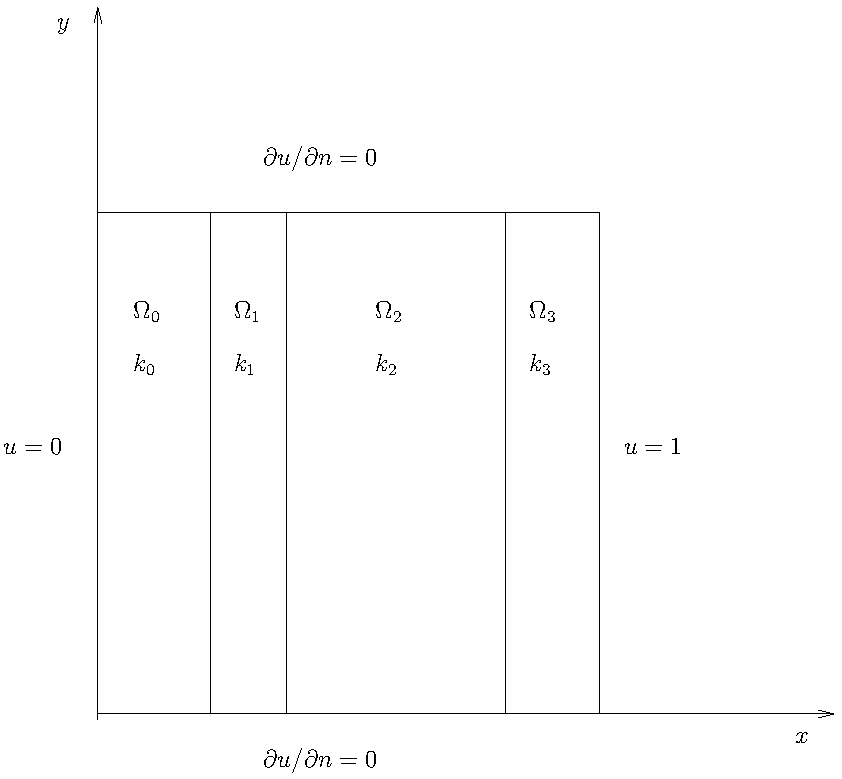
\includegraphics[width=0.7\linewidth]{chapters/langtangen/pdf/layers.pdf}
    }
    \caption{Sketch of a multi-material problem.}
    \label{langtangen:possion:nD:nmat:fig1}
  \end{center}
\end{figure}
Although the sketch of the domain is in two dimensions, we can easily
define this problem in any number of dimensions, using
the ideas of Chapter~\ref{langtangen:poisson:nD}, but the layer
boundaries are planes $x_0=\hbox{const}$ and $u$ varies with
$x_0$ only.

The PDE reads
\begin{equation} \label{langtangen:poisson:2D:varcoeff2}
    \nabla\cdot (k\nabla u) =0 \langtangenep
\end{equation}
To construct a problem where we can find an analytical solution that can
be computed to machine precision regardless of the element size,
we choose $\Omega$ as a hypercube $[0,1]^d$, and the materials as
layers in the $x_0$ direction, as depicted in
Figure~\ref{langtangen:possion:nD:nmat:fig1} for a 2D case with four materials.
The boundaries $x_0=0$ and $x_0=1$ have Dirichlet conditions
$u=0$ and $u=1$, respectively, while Neumann conditions
$\partial u/\partial n=0$ are set on the remaining boundaries.
The complete boundary-value problem is then
\begin{equation} \label{langtangen:poisson:2D:varcoeff3}
  \begin{array}{rcll}
    \nabla\cdot \left(k(x_0)\nabla u(x_0,\ldots,x_{d-1})\right)
      &=& 0 &\mbox{in } \Omega, \\
    u &=& 0 &\mbox{on } \Gamma_0,\\
    u &=& 1 &\mbox{on } \Gamma_1,\\
    {\partial u\over\partial n} &=& 0 &\mbox{on } \Gamma_N\langtangenep
  \end{array}
\end{equation}
The domain $\Omega$ is divided into $s$ materials $\Omega_i$, $i=0,\ldots,s-1$,
where
\[ \Omega_i = \{ (x_0,\ldots,x_{d-1}\, |\, L_i \leq x_0 < L_{i+1}\} \]
for given $x_0$ values $0=L_0<L_1<\cdots< L_s=1$
of the material (subdomain) boundaries.
The $k(x_0)$ function takes on the value $k_i$ in $\Omega_i$.

The exact solution of the basic PDE in \langtangenrefeq{langtangen:poisson:2D:varcoeff3} is
\[ u(x_0,\ldots,x_{d-1}) =
{\int_0^{x_0} (k(\tau ))^{-1}d\tau\over \int_0^1 (k(\tau ))^{-1}d\tau}\langtangenep
\]
For a piecewise constant $k(x_0)$ as explained, we get
\begin{equation}
u(x_0,\ldots,x_{d-1}) =
{(x_0-L_i)k_i^{-1} + \sum_{j=0}^{i-1} (L_{j+1}-L_j)k_j^{-1}\over
\sum_{j=0}^{s-1} (L_{j+1}-L_j)k_j^{-1}},\quad L_i\leq x_0 \leq L_{i+1}\langtangenep
\label{langtangen:poisson:2D:varcoeff2:exact}
\end{equation}
That is, $u(x_0,\ldots,x_{d-1})$ is piecewise linear in $x_0$ and
constant in all other directions.
If $L_i$
coincides with the element boundaries, any standard finite element method
will reproduce this exact solution to machine precision, which is ideal
for a test case.

\hpl{This should be implemented in terms of classes...}

%SHOULD WE HAVE A CLASS INSTEAD? Or functions? No, class, and a module
%where both the preprocess step and the solve step and special BCs
%are handled. Separate general and special pieces of the problem and
%the implementation such that the code can easily be resued
%in a different problem (different PDE, different BCs, different domain).
%class BC with essential and natural conditions, class Domain
%($k$ sits in domain - or in PDE or in Problem?),
%class PDE, and class Problem that has all of them.
%But illustrate this first for a simpler problem!


\subsection{Preparing a Mesh with Subdomains}
\label{langtangen:possion:nD:nmat:prepro}

Our first task is to generate a mesh for $\Omega = [0,1]^d$ and divide
it into subdomains
\[ \Omega_i = \{ (x_0,\ldots,x_{d-1})\, |\, L_i<x_0<L_{i+1}\}\]
for given subdomain boundaries $x_0=L_i$, $i=0,\ldots,s$, $L_0=0$, $L_s=1$.
Note that the boundaries $x_0=L_i$ are points in 1D, lines in 2D, and
planes in 3D.

Let us, on the command line, specify the polynomial degree of Lagrange
elements and the number of element divisions in the various space
directions, as explained in detail in
Chapter~\ref{langtangen:poisson:nD}. This results in an instance {\fontsize{12pt}{12pt}\texttt{mesh}}
representing the interval $[0,1]$ in 1D, the unit square in 2D, or the
unit cube in 3D.

The subdomains $\Omega_i$ must be defined through subclasses
of {\fontsize{12pt}{12pt}\texttt{SubDomain}}. Would could, in principle,
introduce one subclass of {\fontsize{12pt}{12pt}\texttt{SubDomain}} for each subdomain, and
this would be feasible if one has a small and fixed number of
subdomains as in the example in Chapter~\ref{langtangen:possion:2D:2mat:problem} with
two subdomains. Our present case is more general as we
have $s$ subdomains. It then makes sense to create one
subclass {\fontsize{12pt}{12pt}\texttt{Material}} of {\fontsize{12pt}{12pt}\texttt{SubDomain}} and have an attribute
to reflect the subdomain (material) number. We use this number
in the test whether a spatial point {\fontsize{12pt}{12pt}\texttt{x}} is inside a subdomain or not:
\begin{Verbatim}[fontsize=\fontsize{10pt}{10pt},tabsize=8,baselinestretch=1.05,
fontfamily=tt,xleftmargin=7mm]
class Material(SubDomain):
    """Define material (subdomain) no. i."""
    def __init__(self, subdomain_number, subdomain_boundaries):
        self.number = subdomain_number
        self.boundaries = subdomain_boundaries
        SubDomain.__init__(self)

    def inside(self, x, on_boundary):
        i = self.number
        L = self.boundaries         # short form (cf. the math)
        if L[i] <= x[0] <= L[i+1]:
            return True
        else:
            return False
\end{Verbatim}
\noindent
The {\fontsize{12pt}{12pt}\texttt{<=}} in the test if a point is inside a subdomain is important as
{\fontsize{12pt}{12pt}\texttt{x}} will equal vertex coordinates in the elements, and many of these
will lie
on the subdomain boundaries. All vertices {\fontsize{12pt}{12pt}\texttt{x}}
in a cell must be lead to a {\fontsize{12pt}{12pt}\texttt{True}} return value from {\fontsize{12pt}{12pt}\texttt{inside}}
for the cell to be a part of a subdomain.

The marking and numbering of all subdomains
goes as follows:
\begin{Verbatim}[fontsize=\fontsize{10pt}{10pt},tabsize=8,baselinestretch=1.05,
fontfamily=tt,xleftmargin=7mm]
cell_entity_dim = mesh.topology().dim()  # = d
subdomains = MeshFunction('uint', mesh, cell_entity_dim)
# Mark subdomains with numbers i=0,1,\ldots,s (=len(L)-1)
for i in range(s):
    material_i = Material(i, L)
    material_i.mark(subdomains, i)
\end{Verbatim}
\noindent
%Note that the subdomain numbers must $0,1,2,\ldots$.

We have now all the geometric information about subdomains in
a {\fontsize{12pt}{12pt}\texttt{MeshFunction}} instance {\fontsize{12pt}{12pt}\texttt{subdomains}}. The subdomain number
of mesh entity number {\fontsize{12pt}{12pt}\texttt{e}}, here cell {\fontsize{12pt}{12pt}\texttt{e}}, is given
by {\fontsize{12pt}{12pt}\texttt{subdomains.values()[e]}}.

The code presented so far had the purpose of preparing a mesh and
a mesh function defining the subdomain. It is smart to put this code
in a separate file, say {\fontsize{12pt}{12pt}\verb!define_layers.py!},
and view the code as a preprocessing step.
We must then store the computed mesh and mesh function in files.
Another program may load the files and perform the actually
actually solve the boundary-value problem.

Storing the mesh itself and the mesh function in XML format is done by
\begin{Verbatim}[fontsize=\fontsize{10pt}{10pt},tabsize=8,baselinestretch=1.05,
fontfamily=tt,xleftmargin=7mm]
file = File('hypercube_mesh.xml.gz')
file << mesh
file = File('layers.xml.gz')
file << subdomains
\end{Verbatim}
\noindent

This preprocessing code knows about the layer geometries and
the corresponding $k$, which
must be propagated to the solver code. One idea is to let the
preprocessing code write a Python module containing
the {\fontsize{12pt}{12pt}\texttt{L}} and {\fontsize{12pt}{12pt}\texttt{k}} lists as well as an implementation of a
function that evaluates the exact solution.
The solver code can import this module to get access to {\fontsize{12pt}{12pt}\texttt{L}},
{\fontsize{12pt}{12pt}\texttt{k}}, and the exact solution (for comparison).
The relevant Python code for generating a Python module may take
the form
\begin{Verbatim}[fontsize=\fontsize{10pt}{10pt},tabsize=8,baselinestretch=1.05,
fontfamily=tt,xleftmargin=7mm]
f = open('u_layered.py', 'w')
f.write("""
import numpy
L = numpy.array(%s, float)
k = numpy.array(%s, float)
s = len(L)-1

def u_exact(x):
    # First find which subdomain x0 is located in
    for i in range(len(L)-1):
        if L[i] <= x <= L[i+1]:
            break

    # Vectorized implementation of summation:
    s2 = sum((L[1:s+1] - L[0:s])*(1.0/k[:]))
    if i == 0:
        u = (x - L[i])*(1.0/k[0])/s2
    else:
        s1 = sum((L[1:i+1] - L[0:i])*(1.0/k[0:i]))
        u = ((x - L[i])*(1.0/k[i]) + s1)/s2
    return u

if __name__ == '__main__':
    # Plot the exact solution
    from scitools.std import linspace, plot, array
    x = linspace(0, 1, 101)
    u = array([u_exact(xi) for xi in x])
    print u
    plot(x, u)
""" % (L, k))
f.close()
\end{Verbatim}
\noindent


\subsection{Solving the PDE Problem}
\label{langtangen:possion:nD:nmat:solve}

The solver program starts with loading a prepared mesh with a mesh
function representing the subdomains:
\begin{Verbatim}[fontsize=\fontsize{10pt}{10pt},tabsize=8,baselinestretch=1.05,
fontfamily=tt,xleftmargin=7mm]
mesh = Mesh('hypercube_mesh.xml.gz')
subdomains = MeshFunction('uint', mesh, 'layers.xml.gz')
\end{Verbatim}
\noindent

The next task is to define the $k$ function as a finite element function.
As we recall from Chapter~\ref{langtangen:possion:2D:2mat:impl}, a $k$ that
is constant in each element is suitable.
We then follow the recipe from Chapter~\ref{langtangen:possion:2D:2mat:impl}
to compute $k$:
\begin{Verbatim}[fontsize=\fontsize{10pt}{10pt},tabsize=8,baselinestretch=1.05,
fontfamily=tt,xleftmargin=7mm]
V0 = FunctionSpace(mesh, 'DG', 0)
k = Function(V0)

# Vectorized calculation
help = numpy.asarray(subdomains.values(), dtype=numpy.int32)
k.vector()[:] = numpy.choose(help, k_values)
\end{Verbatim}
\noindent

The essential boundary conditions are defined in the same way is
in {\fontsize{12pt}{12pt}\verb!Poisson2D_DN2.py!} from Chapter~\ref{langtangen:poisson:multiple:Dirichlet}
and therefore not repeated here.
The variational problem is defined and solved in a standard manner,
\begin{Verbatim}[fontsize=\fontsize{10pt}{10pt},tabsize=8,baselinestretch=1.05,
fontfamily=tt,xleftmargin=7mm]
v = TestFunction(V)
u = TrialFunction(V)
f = Constant(mesh, 0)
a = k*dot(grad(v), grad(u))*dx
L = v*f*dx

problem = VariationalProblem(a, L, bc)
u = problem.solve()
\end{Verbatim}
\noindent

Plotting the discontinuous {\fontsize{12pt}{12pt}\texttt{k}} is often desired. Just a {\fontsize{12pt}{12pt}\texttt{plot(k)}}
makes a continuous function out of {\fontsize{12pt}{12pt}\texttt{k}}, which is not what we want.
Making a {\fontsize{12pt}{12pt}\texttt{MeshFunction}} over cells and filling in the right $k$
values results in an object that can be displayed as a discontinuous field.
A relevant code is
\begin{Verbatim}[fontsize=\fontsize{10pt}{10pt},tabsize=8,baselinestretch=1.05,
fontfamily=tt,xleftmargin=7mm]
k_meshfunc = MeshFunction('double', mesh, mesh.topology().dim())

# Scalar version
for i in range(len(subdomains.values())):
    k_meshfunc.values()[i] = k_values[subdomains.values()[i]]

# Vectorized version
help = numpy.asarray(subdomains.values(), dtype=numpy.int32)
k_meshfunc.values()[:] = numpy.choose(help, k_values)

plot(k_meshfunc, title='k as mesh function')
\end{Verbatim}
\noindent
The file {\fontsize{12pt}{12pt}\verb!Poisson_layers.py!} contains the complete code.


\section{Miscellaneous Topics}

\subsection{Glossary}

\newcommand{\gln}{\vspace{2mm}\par}

Below we explain some key terms used in this tutorial.

\fenics: name of a software suite composed of many individual software
components (see {\fontsize{12pt}{12pt}\texttt{fenics.org}}). Some components are \dolfin{} and
Viper, explicitly referred to in this tutorial. Others are
FFC and FIAT, heavily used by the programs appearing in this tutorial,
but never explicitly used from the programs.\gln

\dolfin: a \fenics{} component, more precisely a C++ library, with
a Python interface, for performing important actions in finite element
programs. \dolfin{} makes use of many other \fenics{} components and
many external software packages.\gln

Viper: a \fenics{} component for quick visualization of finite element
meshes and solutions.\gln

UFL: a \fenics{} component implementing the \emph{unified form language}
for specifying finite element forms in \fenics{} programs.
The definition of the forms, typically called {\fontsize{12pt}{12pt}\texttt{a}} and {\fontsize{12pt}{12pt}\texttt{L}} in
this tutorial, must have legal UFL syntax. The same applies to
the definition of functionals (see Chapter~\ref{langtangen:poisson1:functionals}).
\hpl{More references to UFL chapter and website!}\gln

Class (Python): a programming construction for creating objects
containing a set of
variables and functions. Most
types of \fenics{} objects are defined through the class concept.\gln

Instance (Python): an object of a particular type, where the type is
implemented as a class. For instance,
{\fontsize{12pt}{12pt}\texttt{mesh = UnitInterval(10)}} creates
an instance of class {\fontsize{12pt}{12pt}\texttt{UnitInterval}}, which is reached by the
the name {\fontsize{12pt}{12pt}\texttt{mesh}}. (Class {\fontsize{12pt}{12pt}\texttt{UnitInterval}} is actually just
an interface to a corresponding C++ class in the \dolfin{} C++ library.)\gln

Class method (Python): a function in a class, reached by dot notation: {\fontsize{12pt}{12pt}\verb!instance_name.method_name!}\gln

{\fontsize{12pt}{12pt}\texttt{self}} parameter (Python): required first parameter in class methods,
representing a particular instance of the class.\langtangenidx{self}
Used in method definitions, but never in calls to a method
For example, if {\fontsize{12pt}{12pt}\texttt{method(self, x)}} is the definition of
{\fontsize{12pt}{12pt}\texttt{method}} in a class {\fontsize{12pt}{12pt}\texttt{Y}}, {\fontsize{12pt}{12pt}\texttt{method}} is called as
{\fontsize{12pt}{12pt}\texttt{y.method(x)}}, where {\fontsize{12pt}{12pt}\texttt{y}} is an instance of class {\fontsize{12pt}{12pt}\texttt{X}}.
In a call like {\fontsize{12pt}{12pt}\texttt{y.method(x)}}, {\fontsize{12pt}{12pt}\texttt{method}} is invoked with
{\fontsize{12pt}{12pt}\texttt{self=y}}.\gln

Class attribute (Python): a variable in a class, reached by dot notation: {\fontsize{12pt}{12pt}\verb!instance_name.attribute_name!}\gln


\subsection{Overview of Objects and Functions}


Most objects in \fenics{} have a explanation of the purpose and usuage
that can be seen by using the general documentation command
{\fontsize{12pt}{12pt}\texttt{pydoc}} for Python objects. You can type\langtangenidx{pydoc}
\begin{Verbatim}[fontsize=\fontsize{10pt}{10pt},tabsize=8,baselinestretch=1.05,
fontfamily=tt,xleftmargin=7mm]
pydoc dolfin.X
\end{Verbatim}
\noindent
to look up documentation of a Python class {\fontsize{12pt}{12pt}\texttt{X}} from the \dolfin{}
library ({\fontsize{12pt}{12pt}\texttt{X}} can be {\fontsize{12pt}{12pt}\texttt{UnitSquare}}, {\fontsize{12pt}{12pt}\texttt{Function}},
{\fontsize{12pt}{12pt}\texttt{Viper}}, etc.). Below is an overview of the most important classes
and functions
in \fenics{} programs, in the order they typically appear within programs.\gln

{\fontsize{12pt}{12pt}\texttt{UnitSquare(nx, ny)}}: generate mesh over the unit square
$[0,1]\times [0,1]$ using {\fontsize{12pt}{12pt}\texttt{nx}} divisions in $x$ direction and
{\fontsize{12pt}{12pt}\texttt{ny}} divisions in $y$ direction. Each of the {\fontsize{12pt}{12pt}\texttt{nx*ny}} squares
are divided into two cells of triangular shape.\gln

{\fontsize{12pt}{12pt}\texttt{UnitInterval}}, {\fontsize{12pt}{12pt}\texttt{UnitCube}}, {\fontsize{12pt}{12pt}\texttt{UnitCircle}}, {\fontsize{12pt}{12pt}\texttt{UnitSphere}},
{\fontsize{12pt}{12pt}\texttt{Interval}}, {\fontsize{12pt}{12pt}\texttt{Rectangle}}, and {\fontsize{12pt}{12pt}\texttt{Box}}: generate mesh over
domains of simple geometric shape, see Chapter~\ref{langtangen:prepro}.\gln

{\fontsize{12pt}{12pt}\verb!FunctionSpace(mesh, element_type, degree)!}:
a function space defined over a mesh, with a given element type
(e.g., {\fontsize{12pt}{12pt}\texttt{'CG'}} or {\fontsize{12pt}{12pt}\texttt{'DG'}}), with basis functions as polynomials of
a specified degree.\gln

{\fontsize{12pt}{12pt}\texttt{Function(V, expression)}}: a scalar- or vector-valued function, given as a
mathematical formula {\fontsize{12pt}{12pt}\texttt{expression}} (string) written in C++ syntax.\gln

{\fontsize{12pt}{12pt}\texttt{Function(V)}}: a scalar- or vector-valued finite element field in
the function space {\fontsize{12pt}{12pt}\texttt{V}}.\gln

{\fontsize{12pt}{12pt}\texttt{SubDomain}}: class for defining a subdomain, either a part of the
boundary, an internal boundary, or a part of the domain.
The programmer must subclass {\fontsize{12pt}{12pt}\texttt{SubDomain}} and implement the
{\fontsize{12pt}{12pt}\verb!inside(self, x, on_boundary)!} function (see Chapter~\ref{langtangen:poisson1:impl}) for telling whether a point {\fontsize{12pt}{12pt}\texttt{x}} is inside the subdomain or not.
\hpl{This will change...}\gln

{\fontsize{12pt}{12pt}\texttt{MeshFunction}}: tool for marking parts of the domain or the boundary.
Used for variable coefficients (``material properties'', see
Chapter~\ref{langtangen:possion:2D:2mat:problem}) or for
boundary conditions (see Chapter~\ref{langtangen:poisson:mat:neumann}).\gln

{\fontsize{12pt}{12pt}\texttt{DirichletBC(V, value, where)}}: specification of Dirichlet (essential)
boundary conditions via a function space {\fontsize{12pt}{12pt}\texttt{V}}, a function
{\fontsize{12pt}{12pt}\texttt{value(x)}} for computing the value of the condition at a point {\fontsize{12pt}{12pt}\texttt{x}},
and a specification {\fontsize{12pt}{12pt}\texttt{where}} of the boundary, either as a
{\fontsize{12pt}{12pt}\texttt{SubDomain}} subclass instance, a plain function, or as a
{\fontsize{12pt}{12pt}\texttt{MeshFunction}} instance.
In the latter case, a 4th argument is provided to describe which subdomain
number that describes the relevant boundary.\gln

{\fontsize{12pt}{12pt}\texttt{TestFunction(V)}}: define a test function on a space {\fontsize{12pt}{12pt}\texttt{V}} to be used
in a variational form.\gln

{\fontsize{12pt}{12pt}\texttt{TrialFunction(V)}}: define a trial function on a space {\fontsize{12pt}{12pt}\texttt{V}} to be used
in a variational form to represent the unknown in a finite element problem.\gln

{\fontsize{12pt}{12pt}\texttt{assemble(X)}}: assemble a matrix, a right-hand side, or a functional,
given a from {\fontsize{12pt}{12pt}\texttt{X}} written with UFL syntax.\gln

{\fontsize{12pt}{12pt}\verb!assemble_system(a, L, bc)!}: assemble the matrix and the right-hand
side from a bilinear ({\fontsize{12pt}{12pt}\texttt{a}}) and linear ({\fontsize{12pt}{12pt}\texttt{L}}) form written with UFL
syntax. The {\fontsize{12pt}{12pt}\texttt{bc}} parameter holds one or more {\fontsize{12pt}{12pt}\texttt{DirichletBC}} instances.\gln

{\fontsize{12pt}{12pt}\texttt{VariationalProblem(a, L, bc)}}: define a variational problem by
a bilinear ({\fontsize{12pt}{12pt}\texttt{a}}) and linear ({\fontsize{12pt}{12pt}\texttt{L}}) form, written with UFL
syntax, and one or more {\fontsize{12pt}{12pt}\texttt{DirichletBC}} instances stored in {\fontsize{12pt}{12pt}\texttt{bc}}.\gln

{\fontsize{12pt}{12pt}\texttt{VariationalProblem(a, L, bc)}}: define and solve a variational problem,
given a bilinear ({\fontsize{12pt}{12pt}\texttt{a}}) and linear ({\fontsize{12pt}{12pt}\texttt{L}}) form, written with UFL
syntax, and one or more {\fontsize{12pt}{12pt}\texttt{DirichletBC}} instances stored in {\fontsize{12pt}{12pt}\texttt{bc}}.
A 4th argument, {\fontsize{12pt}{12pt}\texttt{nonlinear=True}}, can be given to define and solve
nonlinear variational problems (see Chapter~\ref{langtangen:nonlinear:Newton:auto}).\gln

{\fontsize{12pt}{12pt}\texttt{solve(A, U, b)}}: solve a linear system with {\fontsize{12pt}{12pt}\texttt{A}} as coefficient
matrix ({\fontsize{12pt}{12pt}\texttt{Matrix}} instance), {\fontsize{12pt}{12pt}\texttt{U}} as unknown ({\fontsize{12pt}{12pt}\texttt{Vector}} instance),
and {\fontsize{12pt}{12pt}\texttt{b}} as right-hand side ({\fontsize{12pt}{12pt}\texttt{Vector}} instance).
Usually, {\fontsize{12pt}{12pt}\texttt{U}} is replaced by {\fontsize{12pt}{12pt}\texttt{u.vector()}}, where
{\fontsize{12pt}{12pt}\texttt{u}} is a {\fontsize{12pt}{12pt}\texttt{Function}} instance representing the unknown finite
element function of the problem, while
{\fontsize{12pt}{12pt}\texttt{A}} and {\fontsize{12pt}{12pt}\texttt{b}} are computed by calls to {\fontsize{12pt}{12pt}\texttt{assemble}}
or {\fontsize{12pt}{12pt}\verb!assemble_system!}.\gln

{\fontsize{12pt}{12pt}\texttt{plot(q)}}: quick visualization of a mesh, function, or mesh function
{\fontsize{12pt}{12pt}\texttt{q}}, using the Viper component in \fenics{}.\gln

{\fontsize{12pt}{12pt}\texttt{interpolate(func, V)}}: interpolate a formula or finite
element function {\fontsize{12pt}{12pt}\texttt{func}}
onto the function space {\fontsize{12pt}{12pt}\texttt{V}}.\gln

{\fontsize{12pt}{12pt}\texttt{project(func, V)}}: project a formula or finite element function {\fontsize{12pt}{12pt}\texttt{func}}
onto the function space {\fontsize{12pt}{12pt}\texttt{V}}.\gln



\subsection{Installing \fenics}
\label{langtangen:app:install}

The \fenics{} software components are available for Linux, Windows and Mac OS
X platforms. Detailed information on how to get \fenics{} running on such
machines are available at the {\fontsize{12pt}{12pt}\texttt{fenics.org}} website.
Here are just some quick descriptions and recommendations by the author.

To make the installation of \fenics{} as painless and reliable as
possible, the reader is strongly recommended to use Ubuntu Linux. Any
standard PC can easily be equipped with Ubuntu Linux, which may live
side by side with either Windows or Mac OS X or another Linux
installation.  Basically, you download
Ubuntu from {\fontsize{12pt}{12pt}\verb!www.ubuntu.com/getubuntu/download!}, burn the file on
a CD, reboot the machine with the CD, and answer some usually
straightforward questions (if necessary). Ubuntu is quite similar to
both Windows 7 and Mac OS X, but to be efficient when doing science
with \fenics{} this author recommends to run programs in a terminal
window and write them in a text editor like Emacs or Vim. You can
employ integrated development environment such as Eclipse, but
intensive \fenics{} developers and users tend to find terminal windows
and plain text editors more user friendly.

Instead of making it possible to boot your machine with the Linux
Ubuntu operating system, you can run Ubuntu in a separate window in
your existing operation system. On Mac, you can use the VirtualBox
software available
from {\fontsize{12pt}{12pt}\texttt{http://www.virtualbox.org}} to run Ubuntu.  On Windows, Wubi
makes a tool that automatically installs Ubuntu on the machine. Just
give a username and password for the Ubuntu installation, and Wubi
performs the rest. You can also use VirtualBox on Windows machines.

Once the Ubuntu window
is up and running, go to the {\fontsize{12pt}{12pt}\texttt{fenics.org}} cite and paste in
the five few lines that are needed to install what you need.

%With Ubuntu on your machine, installing \fenics{} is a matter of
%cutting and pasting five lines from {\fontsize{12pt}{12pt}\verb!www.fenics.org/wiki/Download!}.

\subsection{Books on the Finite Element Method}
\label{langtangen:appendix:books}
There are a large number of books on the finite element method.
The books typically fall in either of two categories: the abstract
mathematical version of the method and the engineering ``structural analysis''
version of the method. \fenics{} builds heavily on concepts in the former
version. Readers who prefer mathematical rigor, and analysis of the
finite element method, will appreciate the texts by
Brenner and Scott \cite{BrennerScott2008}, Braess \cite{Braess2007}, or
Ciarlet \cite{Ciarlet2002a}.
Alternative books with
less mathematical rigor and more intuitive and engineering-oriented
expositions are ..............
\hpl{Need to find titles.}

%Therefore, books on the
%engineering ``structural analysis'' version of the finite element method
%will be of limited help.

\subsection{Books on Python}
\label{langtangen:appendix:pybooks}

Two very popular introductory books on Python are
``Learning Python''  by Lutz \cite{Lutz2007} and
``Practical Python''  by Hetland \cite{Hetland2002}.
More advanced and comprehensive books include
``Programming Python'' by Lutz \cite{Lutz2006},
and ``Python Cookbook'' \cite{MartelliAscher2005} and ``Python in a Nutshell''
\cite{Martelli2006} by Martelli.
The web page {\fontsize{12pt}{12pt}\texttt{http:://python.org/...}} lists numerous additional
books.
Very few texts teach Python in a mathematical and numerical context,
but the references \cite{Langtangen2009,Langtangen2009b} are exceptions.



\subsection{User-Defined Function Objects}
\label{langtangen:app:cpp:functions}

User-defined functions are implemented as a {\fontsize{12pt}{12pt}\texttt{Function}} object.
There are several ways of constructing such objects, such as
\begin{itemize}
\item a string containing a mathematical expression,
\item a subclass of {\fontsize{12pt}{12pt}\texttt{Function}} in Python,
\item a subclass of {\fontsize{12pt}{12pt}\texttt{Function}} in C++,
\item a set of degrees of freedom of a finite element function.
\end{itemize}
Writing {\fontsize{12pt}{12pt}\texttt{pydoc dolfin.Function}} gives a documentation of the various
techniques.

When defining a function in terms of a mathematical expression inside
a string formula, the expression will be turned into a C++ function
and compiled to gain efficiency. Therefore,
the syntax used in the expression must be valid C++ syntax.
Most Python syntax for mathematical expressions are also valid C++ syntax,
but power expressions make an exception: {\fontsize{12pt}{12pt}\texttt{p**a}} must be written as
{\fontsize{12pt}{12pt}\texttt{pow(p,a)}} in C++ (this is also an alternative Python syntax).
The following mathematical functions can be used directly
in C++
expressions for {\fontsize{12pt}{12pt}\texttt{Function}} objects:
{\fontsize{12pt}{12pt}\texttt{cos}}, {\fontsize{12pt}{12pt}\texttt{sin}}, {\fontsize{12pt}{12pt}\texttt{tan}}, {\fontsize{12pt}{12pt}\texttt{acos}}, {\fontsize{12pt}{12pt}\texttt{asin}},
{\fontsize{12pt}{12pt}\texttt{atan}}, {\fontsize{12pt}{12pt}\texttt{atan2}}, {\fontsize{12pt}{12pt}\texttt{cosh}}, {\fontsize{12pt}{12pt}\texttt{sinh}}, {\fontsize{12pt}{12pt}\texttt{tanh}}, {\fontsize{12pt}{12pt}\texttt{exp}},
{\fontsize{12pt}{12pt}\texttt{frexp}}, {\fontsize{12pt}{12pt}\texttt{ldexp}}, {\fontsize{12pt}{12pt}\texttt{log}}, {\fontsize{12pt}{12pt}\texttt{log10}}, {\fontsize{12pt}{12pt}\texttt{modf}},
{\fontsize{12pt}{12pt}\texttt{pow}}, {\fontsize{12pt}{12pt}\texttt{sqrt}}, {\fontsize{12pt}{12pt}\texttt{ceil}}, {\fontsize{12pt}{12pt}\texttt{fabs}}, {\fontsize{12pt}{12pt}\texttt{floor}}, and {\fontsize{12pt}{12pt}\texttt{fmod}}.
Moreover, the number $\pi$ is available as the symbol {\fontsize{12pt}{12pt}\texttt{pi}}.
All the listed functions are taken from the {\fontsize{12pt}{12pt}\texttt{cmath}} C++ header file, and
one may hence
consult documentation of {\fontsize{12pt}{12pt}\texttt{cmath}} for more information on the
various functions.


\paragraph{Acknowledgments.}
The author is very thankful to Johan Hake, Anders Logg,
Kent-Andre Mardal, and Kristian Valen-Sendstad
for promptly answering all my questions about
\fenics{} functionality and for implementing all my requests.
Professor Douglas Arnold is thanked for valuable feedback on
this tutorial.
